\documentclass[%
	11pt,%
	ngerman,%
]{book}

\usepackage[ngerman]{babel}
\usepackage[utf8]{inputenc}

\usepackage[T1]{fontenc}
\usepackage{microtype}
\usepackage{libertine}
\usepackage{dingbat}

\usepackage[title]{appendix}

\usepackage{printlen}
\usepackage[margincaption,outercaption]{sidecap}
\usepackage[a4paper, %showframe,
 inner=23mm, bottom=4cm, top=3cm,
 outer=52mm, marginparwidth=37mm, marginparsep=5mm
]{geometry}
\linespread{1.1}
\newlength{\margintotalwidth}
\setlength{\margintotalwidth}{\dimexpr\marginparwidth+\marginparsep\relax}

\usepackage[table,dvipsnames]{xcolor}

\usepackage{amsmath}
\usepackage{amsfonts}
\usepackage{amssymb}
\usepackage{nicefrac}
\usepackage{mathtools}
\usepackage{etextools}
\usepackage{tocvsec2}
%\usepackage{keyfloat}


\usepackage[group-separator={,},binary-units=true,exponent-product = \cdot, output-product = \cdot]{siunitx}

%\usepackage{polyglossia}
%\setdefaultlanguage{english}
%\setotherlanguage{german}

% Do not change the order of usepackages in the following block; YOU HAVE BEEN WARNED!
\makeatletter  
	\let\saved@bibitem\@bibitem  
\makeatother  
\usepackage{bibentry}  
\usepackage[hidelinks]{hyperref}  
\usepackage[ngerman]{cleveref}
\Crefname{algocf}{Algorithmus}{Algorithmen}
\crefname{algocf}{Alg.}{Algs.}

\usepackage{environ}


\usepackage{tikz}
\usetikzlibrary{arrows, backgrounds}
\usetikzlibrary{shapes.geometric}
\usetikzlibrary{shapes.multipart}
\usetikzlibrary{arrows.meta}
\usetikzlibrary{shapes.arrows}
\usetikzlibrary{decorations.pathmorphing}
\usetikzlibrary{calc}
\usetikzlibrary{shapes}
\usetikzlibrary{patterns}
\usetikzlibrary{decorations.pathreplacing}
\usetikzlibrary{calligraphy}

\tikzset{snake it/.style={decorate, decoration=snake}}
\tikzstyle{vertex}=[fill=white,draw,circle,minimum size=18pt,inner sep=0pt]
\tikzstyle{inode}=[fill=white,draw,circle,minimum size=18pt,inner sep=0pt]
\tikzstyle{leaf}=[fill=white,draw,inner sep=1mm]
\tikzstyle{bigleaf}=[fill=white,draw,inner sep=1mm,minimum size=16pt]
\usepackage{tikzscale}

\makeatletter
\newcommand{\removelatexerror}{\let\@latex@error\@gobble}
\makeatother

\usepackage{adjustbox}
\usepackage{booktabs}

\usepackage{wrapfig}
\usepackage{graphicx}
\usepackage{subcaption}
\usepackage{ifthen}
\usepackage{etoolbox}
\usepackage{xspace}

\usepackage{enumitem}

\usepackage{makeidx}
\makeindex


\usepackage{url}

\usepackage{tabularx}

% Texroot: skript.tex
\usepackage{xpatch}

% Colors
\definecolor{dunkelgrau}{cmyk}{0,0,0, 0.75} %{0.25, 0.25, 0.30, 0.75}
\definecolor{goetheblau}{cmyk}{1.00, 0.20, 0.00, 0.40}
\definecolor{hellgrau}  {cmyk}{0.04, 0.04, 0.05, 0.02}
\definecolor{sandgrau}  {cmyk}{0.12, 0.09, 0.13, 0.00}
\definecolor{purple}    {cmyk}{0.08, 1.00, 0.30, 0.36}
\definecolor{emorot}    {cmyk}{0.04, 1.00, 0.80, 0.07}
\definecolor{senfgelb}  {cmyk}{0.01, 0.25, 1.00, 0.05}
\definecolor{gruen}     {cmyk}{0.62, 0.40, 0.87, 0.09}
\definecolor{magenta}   {cmyk}{0.08, 0.86, 0.12, 0.12}
\definecolor{orange}    {cmyk}{0.00, 0.70, 1.00, 0.04}
\definecolor{sonnengelb}{cmyk}{0.00, 0.12, 0.95, 0.00}
\definecolor{hellgruen} {cmyk}{0.04, 0.17, 0.81, 0.07}
\definecolor{lichtblau} {cmyk}{0.80, 0.00, 0.06, 0.04}
\colorlet{tablegrey}{sandgrau!50}
\colorlet{sidecolor}{dunkelgrau}
\colorlet{labelcolor}{goetheblau}

\colorlet{fillColor}{goetheblau!30}
\colorlet{fillColorAlt}{sandgrau}
\colorlet{fillColorStrong}{emorot!40}
\colorlet{frontColor}{black}
\colorlet{frontColorAlt}{goetheblau}
\colorlet{frontColorStrong}{emorot}

\colorlet{color1}{goetheblau}
\colorlet{color2}{emorot}
\colorlet{color3}{orange}
\colorlet{color4}{senfgelb}
\colorlet{color5}{lichtblau}


% Header/Footer	
\usepackage{fancyhdr}
\fancyhf{}
\def\headerFormat{\sffamily\color{dunkelgrau}}
\def\defaultPageStyle{
	\pagestyle{fancy}
	\fancyhead[RO]{\headerFormat\nouppercase{\rightmark}}
	\fancyfoot[LE,RO]{\headerFormat\thepage}
}
\defaultPageStyle
\xpretocmd\headrule{\color{dunkelgrau}}{}{\PatchFailed}

\renewcommand{\sectionmark}[1]{\markright{#1}}
\renewcommand{\subsectionmark}[1]{}
\setcounter{secnumdepth}{3}

% Side nodes
\usepackage{marginnote}
\usepackage{sidenotes}
\usepackage[font={small}, labelfont={sf,color=labelcolor},textfont={sf}]{caption}
\renewcommand*{\marginfont}{\small\color{sidecolor}\sffamily\slshape}
\newcommand{\aside}[2][0pt]{\marginnote{#2}[#1]}
\sidecaptionvpos{figure}{t}
\sidecaptionvpos{table}{t}
\renewcommand*\sidecaptionrelwidth{0.75}
\captionsetup[table]{format=plain, font={color=sidecolor,small}}
\DeclareCaptionStyle{marginfigure}{format=plain, labelfont={sf,color=labelcolor,small}, textfont={sl,sf,small}}
\DeclareCaptionStyle{sidecaption}{format=plain, font={color=sidecolor, small}, labelfont={sf,color=labelcolor}, textfont={sl,sf}}
\DeclareCaptionStyle{sidecapfmt}{format=plain, font={color=sidecolor, small}, labelfont={sf,color=labelcolor}, textfont={sl,sf}}

\usepackage{refcount}% http://ctan.org/pkg/refcount
\newcounter{oddpagecheck}
\makeatletter
\newcommand{\ifoddpageelse}{% \ifoddpage{<odd>}{<even>}
	\stepcounter{oddpagecheck}% For unique labels
	\label{opc-\theoddpagecheck}% Place label
	\ifodd\getpagerefnumber{opc-\theoddpagecheck}
		\expandafter\@firstoftwo% Page is odd
	\else
		\expandafter\@secondoftwo% Page is not odd (even)
	\fi}
\makeatother

\newenvironment{widefigure}[1][t]{%
	\begin{figure}[#1]
		\ifoddpageelse{}{\hspace{-\margintotalwidth}}
		\begin{minipage}{\textwidth+\margintotalwidth}
			}{
		\end{minipage}
	\end{figure}
}


\newenvironment{widetable}[1][t]{%
	\begin{table}[#1]
		\ifoddpageelse{}{\hspace{-\margintotalwidth}}
		\begin{minipage}{\textwidth+\margintotalwidth}
			}{
		\end{minipage}
	\end{table}
}

\newenvironment{widebox}[1][\margintotalwidth]{%
	\ifoddpageelse{}{\hspace{\dimexpr-#1\relax}}%
	\begin{minipage}{\textwidth+#1}%
		}{%
	\end{minipage}%
}

\newenvironment{widemath}[1][\margintotalwidth]{%
	\ifoddpageelse{}{\hspace{\dimexpr-#1\relax}}%
	\begin{minipage}{\textwidth+#1}%
		}{%
	\end{minipage}%
}

\newcommand{\raggedinner}{\ifoddpageelse{\raggedright}{\raggedleft}}
\newcommand{\raggedouter}{\ifoddpageelse{\raggedleft}{\raggedright}}


% Pseudo code
\usepackage[ruled,vlined,linesnumbered]{algorithm2e}
\DontPrintSemicolon
\SetAlFnt{\small}

\newcommand{\mycommentsty}[1]{\textcolor{goetheblau}{\sffamily #1}}
\SetCommentSty{mycommentsty}

\newcommand{\mydatasty}[1]{{\sffamily \textsc{\textcolor{gruen}{#1}}}}
\SetDataSty{mydatasty}

\newcommand{\mykwfunctiondatasty}[1]{\textsc{#1}}
\SetFuncSty{mykwfunctiondatasty}


\usepackage{newfloat}

\DeclareFloatingEnvironment[fileext=algflt,placement={!ht},name=Algorithm]{algoflt}
\urlstyle{sf}

% Theorems et al.
\RequirePackage{amsthm}
\usepackage{thmtools}
\usepackage{thm-restate}
\usepackage{mdframed}


\declaretheoremstyle[
	headfont={\sffamily\color{labelcolor}},
	headpunct=\textcolor{labelcolor}{.},
	postheadspace=1em,
	qed=\textcolor{labelcolor}{$\blacktriangleleft$}
]{endmarker}

\declaretheorem[style=endmarker, parent=chapter]{theorem}
\declaretheorem[style=endmarker, numbered=no, name=Theorem]{theorem*}

\declaretheorem[style=endmarker, numberlike=theorem]{definition}
\declaretheorem[style=endmarker, numbered=no, name=Definition]{definition*}
\declaretheorem[style=endmarker, numberlike=theorem]{corollary}
\declaretheorem[style=endmarker, numbered=no, name=Korollar]{corollary*}
\declaretheorem[style=endmarker, numberlike=theorem]{lemma}
\declaretheorem[style=endmarker, numbered=no, name=Lemma]{lemma*}
\declaretheorem[style=endmarker, numberlike=theorem]{proposition}
\declaretheorem[style=endmarker, numbered=no, name=Proposition]{proposition*}
\declaretheorem[style=endmarker, numberlike=theorem]{conjecture}
\declaretheorem[style=endmarker, numbered=no, name=Conjecture]{conjecture*}
\declaretheorem[style=endmarker, numberlike=theorem]{example}
\declaretheorem[style=endmarker, numbered=no, name=Example]{example*}
\declaretheorem[style=endmarker, numbered=no, name=Note]{note*}
\declaretheorem[style=endmarker, numberlike=theorem, name=Beobachtung]{observation}
\declaretheorem[style=endmarker, numbered=no, name=Beobachtung]{observation*}
\declaretheorem[style=endmarker, numberlike=theorem]{remark}
\declaretheorem[style=endmarker, numbered=no, name=Remark]{remark*}
\declaretheorem[style=endmarker, numberlike=theorem, name=Aufgabe]{exercise}
\declaretheorem[style=endmarker, numbered=no, name=Aufgabe]{exercise*}

\declaretheorem[style=endmarker, numberlike=theorem,
	%	mdframed={backgroundcolor=black!10, linecolor=labelcolor, topline=false,rightline=false},
	qed={},
	name={Case Study}]{casestudy}

\declaretheorem[style=endmarker, numberlike=theorem, mdframed={
			backgroundcolor=black!10,
			linecolor=labelcolor,
			topline=false,rightline=false},
	qed={},
	name={Example}]{introexample}

\expandafter\let\expandafter\oldproof\csname\string\proof\endcsname
\let\oldendproof\endproof
\renewenvironment{proof}[1][\proofname]{%
	\renewcommand\qedsymbol{\textcolor{goetheblau}{$\square$}}
	\oldproof[\normalfont\textcolor{goetheblau}{\sffamily #1}]%
}{\oldendproof}



\RequirePackage{aliascnt}
\usepackage{titlesec}
\usepackage{mathrsfs}
\usepackage{multirow}


\newcommand{\fmtLabel}[1]{\textcolor{darkgray}{\sffamily\bfseries #1}}

\makeatletter
\renewcommand\section{\@startsection {section}{1}{\z@}%
  {-3.5ex \@plus -1ex \@minus -.2ex}%
  {2.3ex \@plus.2ex}%
  {\sffamily\large\bfseries\raggedright}}
\renewcommand\subsection{\@startsection{subsection}{2}{\z@}%
	{-3.25ex\@plus -1ex \@minus -.2ex}%
	{1.5ex \@plus .2ex}%
	{\sffamily\large\bfseries\raggedright}}
\renewcommand\subsubsection{\@startsection{subsubsection}{3}{\z@}%
	{-3.25ex\@plus -1ex \@minus -.2ex}%
	{1.5ex \@plus .2ex}%
	{\sffamily\large\bfseries\raggedright}}
\renewcommand\paragraph{\@startsection{paragraph}{4}{\z@}%
	{-3.25ex \@plus-1ex \@minus-.2ex}%
	{1.5ex \@plus .2ex}%
	{\sffamily\large\bfseries\raggedright}}
\renewcommand\subparagraph{\@startsection{subparagraph}{5}{\z@}%
	{3.25ex \@plus1ex \@minus .2ex}%
	{-1em}%
	{\sffamily\normalsize\bfseries}}
\makeatother



\usepackage{listings}% http://ctan.org/pkg/listings
\lstset{
	basicstyle=\ttfamily,
	mathescape
}


\makeatletter
\newenvironment{relatedbib}{%
	\begingroup%
	\makeatletter%
	\let\@bibitem\saved@bibitem%
	\nobibliography*%
	\begin{itemize}%
		\def\sc{} % PREVENT AUTHORS IN SC
		\def\bibentryitem##1{\item[\cite{##1}] \bibentry{##1} .}%
		      \def\bibentryitemaside##1##2{\item[\cite{##1}]\aside{##2}\bibentry{##1} .}%
		      }{%
	\end{itemize}%
	\endgroup%
}

\colorlet{chapterDigitColor}{dunkelgrau!50}

\newcommand{\chapterTitlePage}[3]{%
	\titleformat{\chapter}[display]
	{}
	{} % label \thechapter
	{0pt} % sep
	{} % before
	[] % after		

	\clearpage{\thispagestyle{empty}\cleardoublepage}
	\chapter[#2]{
	  \vspace{-3cm}
	  \begin{tikzpicture}
		  \node[anchor=south east, chapterDigitColor, inner sep=0] (cpt-mark) {\begin{minipage}{1.25\textwidth}\raggedleft\scalebox{5}{\Huge \thechapter}\end{minipage}};
		  \node[font={\huge}, anchor=south west, at=(cpt-mark.south west), inner sep=0] (cpt-title) {\begin{minipage}{\textwidth}\sffamily#3\end{minipage}};
	  \end{tikzpicture}
	 }
	\label{cpt:#1}
	\thispagestyle{empty}
}


\newenvironment{paperfrontmatter}[1]{%
	\def\@chapter@title{}
	\def\@chapter@runninTitle{}
	\def\@chapter@abstract{}
	\def\@chapter@remarks{}
	\let\@chapter@authors\relax
	\def\@chapter@basedon{}
	\let\@chapter@contribution\relax

	\newcommand{\cTitle}[1]{\gdef\@chapter@title{##1}}
	\newcommand{\cAuthors}[1]{\gdef\@chapter@authors{##1}}
	\newcommand{\cRunningTitle}[1]{\gdef\@chapter@runningTitle{##1}}
	\newcommand{\cAbstract}[1]{\long\gdef\@chapter@abstract{##1}}
	\newcommand{\cRemarks}[1]{\long\gdef\@chapter@remarks{##1}}
	\newcommand{\cBasedOn}[1]{\gdef\@chapter@basedon{##1}}
	\newcommand{\cContribution}[1]{\gdef\@chapter@contribution{##1}}

	\newcommand{\paperChapterTitlePage}{%
		\chapterTitlePage{#1}{\@chapter@runningTitle}{\@chapter@title}
		\ifthenelse{\equal{\@chapter@authors}{}}{%
			\vspace{-5em}%
		}{%
			\vspace{-5em}%
			{
				\linespread{1.3}
				\sffamily joint work with \@chapter@authors\par
			}
			\vspace{1em}%
		}%
		\vfill
		\hfill
		\begin{minipage}{0.96\textwidth}%
			\sffamily%
			\@chapter@abstract
		\end{minipage}%
		%		
		\vfill\vfill
		\noindent%		
		\@chapter@remarks
		\begin{relatedbib}
			\foreach \x in \@chapter@basedon {\bibentryitem{\x}}
		\end{relatedbib}
		\ifx\@chapter@contribution\relax\else
			\vfill
			\subsubsection*{My contribution}
			\@chapter@contribution
		\fi
		%	
		\vfill\vfill
		\vfill\vfill
		%	
		\clearpage%
	}
}{%
	\paperChapterTitlePage%
}

\newcommand{\startpaper}[1]{%
	\fancyhead[LE]{\headerFormat\@chapter@runningTitle}%
}

\makeatother

\colorlet{DarkGreen}{green}
\colorlet{DarkBlue}{blue}
\colorlet{DarkRed}{red}

\tikzset{snake it/.style={decorate, decoration=snake}}
\tikzset{onif/.code args={<#1>#2}{\ifthenelse{#1}{\pgfkeysalso{#2}}{}}}
\tikzset{
conflict/.style={DarkRed, fill=red!10},
state1/.style={DarkGreen, fill=green!10},
state2/.style={DarkBlue, fill=blue!5},
state3/.style={Maroon, fill=Yellow!10},
state4/.style={Red, fill=Thistle!30},
state5/.style={Black, fill=black!5},
state?/.style={conflict}
}
\def\arrowHead{Latex[length=0.5em, width=0.5em]}

\newcommand{\labelfmt}[1]{\textcolor{labelcolor}{\textsl{#1}}}

\newcommand{\seeref}[1]{\leftpointright~\cref{#1}}
\newcommand{\qremark}[1]{\labelfmt{[#1]}\xspace}
\newcommand{\qmremark}[1]{\text{\textcolor{labelcolor}{\ensuremath{#1}}}}
\renewcommand{\path}[1]{\IfSubStr{#1}{_}{\StrSubstitute{#1}{_}{\_}}{#1}}


\newcommand{\reffmt}[1]{\textcolor{labelcolor}{#1}}
\newcommand{\labrefint}[4]{\reffmt{#1:} #2 \reffmt{\seeref{#3} #4}\\}
\newcommand{\labref}[3][]{\labrefint{#2}{\\}{#3}{#1}}
\newcommand{\labrefff}[2]{\labrefint{#1}{\\}{#2}{ff.}}
\newcommand{\sidelabref}[2]{\aside{\labref{#1}{#2}}}

\newenvironment{subapx}{
	\addcontentsline{toc}{section}{Appendix}
	\begin{subappendices}
		\settocdepth{chapter}
		}{
		\resettocdepth
	\end{subappendices}
}

\newcommand{\floatmarginfigure}[1]{
	\begin{figure}[h]%
		\aside{\ \par \vspace{-0.5em} #1}%
		\vspace{-1.5em}
	\end{figure}
}
\makeatother

\newcommand{\varn}[1]{\textsl{#1}}

\newcommand{\crefApx}[1]{\cref{#1} (Appendix)}
\newcommand{\CrefApx}[1]{\Cref{#1} (Appendix)}

\newcommand{\hc}[1]{#1}
\newcommand{\hcm}[1]{\hc{\ensuremath{#1}}\xspace}
\newcommand{\hcs}[1]{\hc{#1}\xspace}
\newcommand{\formatIdentifier}[1]{\hcm{\mathsf{#1}}}

\renewcommand{\epsilon}{\varepsilon}
\newcommand{\remove}[1]{}

\newcommand{\lbbfs}{{\cal D}_{\mathrm{BFS}(v)}}
\newcommand{\size}{\mathrm{size}}
\newcommand{\dpth}{\mathrm{depth}}
\newcommand{\maxdpth}{\overline{\dpth}}


\DeclareMathOperator{\polylog}{poly\,log}
\DeclareMathOperator{\sort}{sort}
\DeclareMathOperator{\scan}{scan}
\DeclareMathOperator{\cdm}{cdm}
\DeclareMathOperator{\acosh}{acosh}
\DeclareMathOperator{\asinh}{asinh}
\let\arccos\relax
\DeclareMathOperator{\arccos}{acos}
\DeclareMathOperator{\odeg}{outDeg}
\DeclareMathOperator{\avg}{avg}

\newcommand{\symOt}{\ensuremath{\tilde{\mathcal{O}}}}
\newcommand{\symOh}{\ensuremath{\mathcal{O}}}
\newcommand{\symoh}{\ensuremath{{o}}}
\newcommand{\symTh}{\ensuremath{\Theta}}
\newcommand{\symOm}{\ensuremath{\Omega}}
\newcommand{\symom}{\ensuremath{\omega}}

\newcommand{\Ot}[1]{\ensuremath{\symOt\!\left(#1\right)}}
\newcommand{\Oh}[1]{\ensuremath{\symOh\!\left(#1\right)}}
\newcommand{\oh}[1]{\ensuremath{\symoh\!\left(#1\right)}}
\newcommand{\Th}[1]{\ensuremath{\symTh\!\left(#1\right)}}
\newcommand{\Om}[1]{\ensuremath{\symOm\!\left(#1\right)}}
\newcommand{\om}[1]{\ensuremath{\symom\!\left(#1\right)}}

\newcommand{\OhSq}[1]{\ensuremath{\symOh\!\left[#1\right]}}

\newcommand{\I}{i}
\newcommand{\setd}[2]{\ensuremath{\left\{#1 \, \middle|\, #2\right\}}}
\newcommand{\acos}{\arccos}


\newcommand{\intd}{\text d}

\newcommand{\e}{\ensuremath{e}}
\newcommand{\errorterm}[1]{#1}%{\textcolor{blue}{ #1 }}
\newcommand{\req}[2]{\ensuremath{\texttt{req}_{#1}(#2)}}

% abbr
% machine models
\newcommand{\nproc}{\ensuremath{P}}

% graph
%\newcommand{\opstyle}[1]{\mathrm{\textcolor{blue}{#1}}}
\newcommand{\opstyle}[1]{\mathrm{#1}}
\newcommand{\degree}{\ensuremath{\opstyle{deg}}}
\newcommand{\degin} {\ensuremath{\opstyle{deg^{in}}}}
\newcommand{\degout}{\ensuremath{\opstyle{deg^{out}}}}
\newcommand{\maxdeg}{\ensuremath{\opstyle{maxdeg}}}
\newcommand{\diam}{\ensuremath{\opstyle{diam}}}
\newcommand{\maxdiam}{\overline{\diam}}
\newcommand{\dist}{\ensuremath{\opstyle{dist}}}
\newcommand{\adj}{\ensuremath{\opstyle{N}}}
\newcommand{\adjin}{\ensuremath{\opstyle{N^{in}}}}
\newcommand{\adjout}{\ensuremath{\opstyle{N^{out}}}}
\newcommand{\degseq}{\ensuremath{\mathcal{D}}}
\newcommand{\cc}{\ensuremath{\opstyle{cc}}}
\newcommand{\density}{\ensuremath{\opstyle{dens}}}

% graph classes
\newcommand{\gGn}{\ensuremath{\mathbb G(n)}\index{$\mathbb G(n)$!set}\xspace} % graphs on n vertices
\newcommand{\gGnm}{\ensuremath{\mathbb G(n,m)}\index{$\mathbb G(n,m)$!set}\xspace} % graphs on n vertices with m edges
\newcommand{\gGnr}{\ensuremath{\mathbb G^{(r)}(n)}\xspace} % r-regular graphs on n vertices
\newcommand{\Gn}{\ensuremath{\mathcal{G}(n)}\index{$G(n)$!uniform distr.}\xspace} % uniform distribution on \gGn
\newcommand{\Gnm}{\ensuremath{\mathcal{G}(n,m)}\index{$G(n,m)$!uniform distr.}\xspace} % uniform distribution on \gGnm
\newcommand{\Gnp}{\ensuremath{\mathcal{G}(n,p)}\index{$\mathcal G(n, p)$}\xspace}
\newcommand{\Gnr}{\ensuremath{\mathcal{G}^{(r)}(n)}\xspace} % uniform distribution on \gGnr

% common sets
\newcommand{\sN}{\ensuremath{\mathbb{N}}}
\newcommand{\sNpos}{\ensuremath{\mathbb{N}_{>0}}}
\newcommand{\sZ}{\ensuremath{\mathbb{Z}}}
\newcommand{\sR}{\ensuremath{\mathbb{R}}}
\newcommand{\NP}{\ensuremath{\mathcal{NP}}}

% prop
\newcommand{\symprob}{\ensuremath{\mathbb{P}}}
\newcommand{\symexpv}{\ensuremath{\mathbb{E}}}
\newcommand{\prob}[1]{\ensuremath{\symprob\!\left[#1\right]}}
\newcommand{\expv}[1]{\ensuremath{\symexpv\!\left[#1\right]}}
\newcommand{\varv}[1]{\ensuremath{\operatorname{Var}\!\left[#1\right]}}
\newcommand{\pld}[3]{\ensuremath{\textsc{Pld}\,([#1, #2), #3)}}
\newcommand{\binomd}[2]{\ensuremath{\text{\textsc{BinD}}\left[#1, #2\right]}}
\newcommand{\geom}[1]{\ensuremath{\opstyle{Geom}(#1)}}
\newcommand{\whp}{whp.\xspace}
\newcommand{\follows}{\sim}


\newcommand{\Def}{\ensuremath{:=}}
\newcommand{\seq}[3]{\ensuremath{[\,#1\,]_{#2}^{#3}}}
\newcommand{\rank}{\ensuremath{\operatorname{rank}}}
\newcommand{\var}{\ensuremath{\operatorname{Var}}}

\newcommand{\mean}[1]{\ensuremath{\left\langle #1 \right\rangle}}
\newcommand{\avgdeg}{\ensuremath{\avg{\degree}}}
\newcommand{\avgdist}{\ensuremath{\avg{\dist}}}

\newcommand{\set}[1]{\ensuremath{\left\{ #1\right\}}}
\newcommand{\floor}[1]{\ensuremath{\left\lfloor #1\right\rfloor}}
\newcommand{\card}[1]{\ensuremath{\lvert #1\rvert}}

\newcommand{\showcomment}[1]{#1}
\renewcommand{\showcomment}[1]{} % Comment in to disable comments
\newcommand{\citeneed}{\showcomment{\ensuremath{^\text{\color{red}{[citation needed]}}}}\xspace}






\usepackage{todonotes}
\newcommand{\TODO}[1]{\todo[inline]{{\footnotesize #1}}}

\newcommand*{\diff}{\mathop{}\!\mathrm{d}}


\newcommand{\invar}[1]{(\texttt{I#1})}

\newcommand{\degs}{\ensuremath{\mathcal D}}
\newcommand{\defrel}{:=}

\newenvironment{lemmarep}[1]{\noindent\textbf{Lemma~\ref{#1}. (repeated)}\itshape}{}
\newcommand{\mult}[1]{\#(#1)}
\newcommand{\moment}[1]{\langle #1 \rangle}

\newcommand{\sequence}[3]{\ensuremath{[\,#1\,]_{#2}^{#3}}}

\DeclareMathOperator{\swap}{\mathtt{swap}}
\DeclareMathOperator{\fst}{fst}
\DeclareMathOperator{\snd}{snd}

\newcommand{\formatImpl}[1]{\textsc{#1}}

\newcommand{\dhrg}{\ensuremath{d_{\mathrm{HRG}}}}
\newcommand{\dgirg}{\ensuremath{d_{\mathrm{GIRG}}}}
\newcommand{\Dgirg}{\ensuremath{D_{\mathrm{GIRG}}}}
\DeclareMathOperator{\level}{level}

\newcommand{\BigO}{\mathcal{O}}
\newcommand{\erdos}{Erd{\H o}s-R{\'e}nyi}

\newcommand{\punkt}{\enspace .}
\newcommand{\komma}{\enspace ,}
\newcommand{\expect}{{\mathbf{E}}}
% asymptotische Notation
\newcommand{\whpO}[1]{\tilde{\mathrm{O}}\left( #1\right)}
\newcommand{\Oschlange}{$\tilde{\mathrm{O}}$}

\newcommand{\Ohh}[1]{\mathcal{O}\!\left( #1\right)}
\newcommand{\Ohsmall}[1]{\mathcal{O}(#1)}
\newcommand{\Thsmall}[1]{\Theta( #1)}
\newcommand{\Omsmall}[1]{\Omega( #1)}
\newcommand{\Oleq}{\preceq}

\newcommand{\CC}{C\raisebox{.08ex}{\hbox{\tt ++}}}
\newcommand{\Cminus}{C\raisebox{.08ex}{\hbox{\tt ++}}\raisebox{.25ex}{-}}
\newcommand{\GG}{g\raisebox{.08ex}{\hbox{\tt ++}}}
\newcommand{\Gminus} {g\raisebox{.08ex}{\hbox{\tt ++}}\raisebox{.25ex}{-}}




\newcommand{\A}{\mathcal A}
\newcommand{\Nei}[1]{\ensuremath{\A_{#1}}}
\newcommand{\AG}{\mathscr{A}_G}
\newcommand{\Suc}{\ensuremath{\mathscr{S}}}
\renewcommand{\O}{\mathcal O} % big O

\newcommand{\hide}[1]{}

\newcommand\myalgorithmCommSty[1]{\footnotesize\ttfamily\textcolor{olive}{#1}}


\let\epsilon\varepsilon


\def\Wlog      {\hcs{W.l.o.g.}\ }
\def\wrt       {\hcs{w.\,r.\,t.}}
\def\etal      {\hcs{et~al.}}
\def\eg        {\hcs{e.g.,}}
\def\cf        {\hcs{cf.}\ }
\def\ie        {\hcs{i.e.,}}
\def\citeneeded{\textsuperscript{\textcolor{red}{[cite needed]}}}

\newcommand{\Ex}[1]{\hcm{\mathbb E\left[#1\right]}}
\newcommand{\Prob}[1]{\hcm{\mathbb P\left[#1\right]}}


\renewcommand{\set}[1]{\hcm{\left\{#1\right\}}}
\newcommand{\problem}[1]{\textsc{#1}}

\DeclareMathOperator{\poly}{poly}


\newcommand*{\LDAUOmicron}[1]{\ensuremath{\operatorname{O}\left(#1\right)}}
\newcommand*{\LDAUomicron}[1]{\ensuremath{\operatorname{o}\left(#1\right)}}
\newcommand*{\LDAUOmega}[1]{\ensuremath{\operatorname{\Omega}\left(#1\right)}}
\newcommand*{\LDAUomega}[1]{\ensuremath{\operatorname{\omega}\left(#1\right)}}
\newcommand*{\LDAUTheta}[1]{\ensuremath{\operatorname{\Theta}\left(#1\right)}}

\newcommand*{\LdauOmicron}[1]{\ensuremath{\operatorname{O}\bigl(#1\bigr)}}
\newcommand*{\Ldauomicron}[1]{\ensuremath{\operatorname{o}\bigl(#1\bigr)}}
\newcommand*{\LdauOmega}[1]{\ensuremath{\operatorname{\Omega}\bigl(#1\bigr)}}
\newcommand*{\Ldauomega}[1]{\ensuremath{\operatorname{\omega}\bigl(#1\bigr)}}
\newcommand*{\LdauTheta}[1]{\ensuremath{\operatorname{\Theta}\bigl(#1\bigr)}}

\newcommand*{\ldauOmicron}[1]{\ensuremath{\operatorname{O}(#1)}}
\newcommand*{\ldauomicron}[1]{\ensuremath{\operatorname{o}(#1)}}
\newcommand*{\ldauOmega}[1]{\ensuremath{\operatorname{\Omega}(#1)}}
\newcommand*{\ldauomega}[1]{\ensuremath{\operatorname{\omega}(#1)}}
\newcommand*{\ldauTheta}[1]{\ensuremath{\operatorname{\Theta}(#1)}}

\newcommand*{\SOFTOmicron}[1]{\ensuremath{\operatorname{\tilde{O}}\left(#1\right)}}
\newcommand*{\SOFTomicron}[1]{\ensuremath{\operatorname{\tilde{o}}\left(#1\right)}}
\newcommand*{\SOFTOmega}[1]{\ensuremath{\operatorname{\tilde{\Omega}}\left(#1\right)}}
\newcommand*{\SOFTomega}[1]{\ensuremath{\operatorname{\tilde{\omega}}\left(#1\right)}}
\newcommand*{\SOFTTheta}[1]{\ensuremath{\operatorname{\tilde{\Theta}}\left(#1\right)}}

\newcommand*{\SoftOmicron}[1]{\ensuremath{\operatorname{\tilde{O}}\bigl(#1\bigr)}}
\newcommand*{\Softomicron}[1]{\ensuremath{\operatorname{\tilde{o}}\bigl(#1\bigr)}}
\newcommand*{\SoftOmega}[1]{\ensuremath{\operatorname{\tilde{\Omega}}\bigl(#1\bigr)}}
\newcommand*{\Softomega}[1]{\ensuremath{\operatorname{\tilde{\omega}}\bigl(#1\bigr)}}
\newcommand*{\SoftTheta}[1]{\ensuremath{\operatorname{\tilde{\Theta}}\bigl(#1\bigr)}}

\newcommand*{\softOmicron}[1]{\ensuremath{\operatorname{\tilde{O}}(#1)}}
\newcommand*{\softomicron}[1]{\ensuremath{\operatorname{\tilde{o}}(#1)}}
\newcommand*{\softOmega}[1]{\ensuremath{\operatorname{\tilde{\Omega}}(#1)}}
\newcommand*{\softomega}[1]{\ensuremath{\operatorname{\tilde{\omega}}(#1)}}
\newcommand*{\softTheta}[1]{\ensuremath{\operatorname{\tilde{\Theta}}(#1)}}

\DeclarePairedDelimiter{\ceil}{\lceil}{\rceil}

\def\?#1{}

%\usepackage{enumitem}
\newenvironment{itemize*}%
{\begin{itemize}%[leftmargin=1.5em]%
		%		\setlength{\itemsep}{0pt}%
		%		\setlength{\parskip}{0pt}%
		%		\setlength{\topsep}{1pt}%
		%		\setlength{\partopsep}{1pt}%
		}{\end{itemize}}

\newenvironment{enumerate*}%
{\begin{enumerate}%[leftmargin=2.5em]%
		%		\setlength{\itemsep}{0pt}%
		%		\setlength{\parskip}{0pt}%
		%		\setlength{\topsep}{1pt}%
		%		\setlength{\partopsep}{1pt}%
		}{\end{enumerate}}


\newenvironment{myalgorithm}[1][htb]
{
	\let\oldnl\nl% Store \nl in \oldnl
	\newcommand{\nonl}{\renewcommand{\nl}{\let\nl\oldnl}}% Remove line number for one line

	\SetCommentSty{myalgorithmCommSty}

	\DontPrintSemicolon
	\SetAlgoLined\SetAlgoNoEnd
	\SetArgSty{normalfont}
	\SetKwInOut{Input}{Input}
	\SetKwInOut{Output}{Output}
	\SetKw{Continue}{continue}
	\SetKwFor{ParForEach}{par foreach}{}{}
	\SetKw{Sequentially}{sequentially}
	\renewcommand{\algorithmcfname}{Algorithm}% Update algorithm name
	\begin{algorithm}[#1]\small%
		}{\end{algorithm}}

\def\mainchapters{\Cref{cpt:pa,cpt:emlfr,cpt:curveball,cpt:hypergen,cpt:commfree,cpt:girgs}}




\title{Network Science und Algorithm Engineering}
\author{Manuel Penschuck}

\begin{document}
\maketitle

\clearpage

\tableofcontents

\chapter{Einleitung}
\glqq Network Science\grqq{} und \glqq Algorithm Engineering\grqq{} sind zwei aktive und interdisziplinäre Forschungsfelder.
Beide Felder sind relativ jung (etwa 20 bis 30 Jahre alt) und haben sich in den letzten Jahren stark weiterentwickelt.
Sie könnten beide unabhängig von einander ganze Studiengänge füllen (und tun es auch).
In dieser Veranstaltung möchten wir also nicht die Vereinigung beider Felder beleuchten, sondern uns einige Themen in ihrem Schnitt ansehen.
Dennoch sollten wir grob die Felder charakterisieren.

\emph{Network Science} beschäftigt sich mit der Analyse und Modellierung von komplexen Netzwerken.
Beispiele sind soziale, Kommunikations- und Verkehrsnetze, biologische Netzwerke und viele mehr.
Sie zeichnen sich durch sogenanntes \emph{emergentes Verhalten} aus: Ohne dass einzelnen Knoten oder Kanten bewusst darauf hinarbeiten, entsteht ein komplexes Verhalten des Gesamtsystems.
In sozialen Netzen bilden sich z.\,B. lokal stark vernetzte Gruppen (Communities), es gibt einige zentrale Teilnehmer, die übermäßig stark vernetzt sind (Celebrities), und Netze haben überraschend geringe Distanzen zwischen Nutzern.
Network Science versucht, diese Eigenschaften zu finden und zu verstehen.
Hierzu vereinigt es Methoden aus Mathematik, Informatik, und Physik.

\vspace{-2em}
\floatmarginfigure{
    \scalebox{0.9}{
        \begin{tikzpicture}[
            box/.style={draw, minimum width=8em, minimum height=2.5em, inner sep=0.2em, align=center},
            arr/.style={draw, >={LaTeX[width=1em,length=1em]}, thick, ->, labelcolor}
            ]
            \node[box] (s0) at (0,  0.0em) {Algorithmen-\\[-0.4em]entwurf};
            \node[box] (s1) at (0, -4.5em) {Theoretische \\[-0.4em] Analyse};
            \node[box] (s2) at (0, -9.0em) {Implementierung};
            \node[box] (s3) at (0,-13.5em) {Experimentelle \\[-0.4em] Analyse};

            \path[arr] (s0) to (s1);
            \path[arr] (s1) to (s2);
            \path[arr] (s2) to (s3);

            \path[arr] (s3.east) to ++(1.5em,0) |- (s0);
            \path[arr] (s3.east) to ++(1.5em,0) |- (s2);
        \end{tikzpicture}}
    \caption{Algorithm Engineering Zyklus}
    \label{fig:intro/algorithm-engineering}}
Ziel des \emph{Algorithm Engineering} ist es, die Spaltung zwischen Theorie und Praxis im Algorithmenentwurf zu überbrücken.
Es geht also darum, theoretisch effiziente als auch praktisch schnelle und implementierbare Algorithmen zu entwickeln.
Hierbei kommt oft die in \cref{fig:intro/algorithm-engineering} dargestellte zyklische Entwurfsmethode zum Einsatz:

Wir entwerfen meist zuerst einen Algorithmus und versuchen, dessen Performance theoretisch vorherzusagen;
diese Hypothesen werden dann experimentell überprüft und -- je nach Ergebnis -- der Algorithmus oder die Analyse (z.\,B. Average Case statt Worst Case) angepasst.
Dieser Zyklus wird wiederholt, bis ein Algorithmus gefunden ist, der sowohl praktisch gut funktioniert als auch theoretisch verstanden ist.

Um praktisch nützliche Vorhersagen treffen zu können, verwendet man im Algorithm Engineering möglichst realistische Modelle für die Maschine und die Eingabedaten.
Zur Analyse von Graphalgorithmen benötigen wir also geeignete Modelle für Netzwerke.
Zur Analyse von großen Netzwerken benötigen wir wiederum effiziente Algorithmen.
So ergänzen sich die beiden Felder.

\section{Über diese Veranstaltung}
Lernziele dieser Veranstaltung beinhalten:
\begin{itemize}
    \item Wichtige Eigenschaften von beobachteten Netzwerken (z.\,B. Dichte, Gradverteilung, Zusammenhang, Durchmesser, lokales Clustering, globales Clustering)
    \item Methoden, diese Eigenschaften nachzubilden und zu erklären
    \item Zufallsgraphen und ihre Eigenschaften
    \item Effiziente Algorithmen für und auf Zufallsgraphen
    \item Effiziente, randomisierte Algorithmen (wir betrachten viele Graphgeneratoren -- die Techniken eignen sich aber viel allgemeiner für diverse Simulationsaufgaben)
\end{itemize}

\section{Begrifflichkeiten}
Ein \emph{Netzwerk} ist ein System, in dem Personen/Agenten/Objekte (etc.) miteinander in Relation stehen (z.\,B. durch eine Freundschaft, ein Gespräch usw.).
\emph{Graphen} sind ein abstraktes Modell dieses Systems: Wir identifizieren die Akteure mit den Knoten und die Beziehungen mit den Kanten.
Wenn wir ein Netzwerk aus der echten Welt in einen Graphen übersetzen, sprechen wir oft von einem \emph{beobachteten Netzwerk}.
Diese Abbildung geht oft mit dem Verlust von Informationen einher (wir wollen für den Anwendungsfall Unwesentliches ausblenden) und ist oft nicht eindeutig.

\begin{example}
    Die akademische Arbeit ist von Kollaboration geprägt -- Wissenschaftler arbeiten zusammen und publizieren schließlich gemeinsam ihre Ergebnisse.
    Es handelt sich also ganz klar um ein Netzwerk.
    Wie modellieren wir aber den zugrunde liegenden Graphen?
    Hier ein paar Ansätze:

    \begin{itemize}
        \item
              Wir können Autoren als Knoten auffassen und eine Kante zwischen zwei Autoren ziehen, wenn sie zusammen publiziert haben.
              Hierbei geht die Information darüber verloren, wie oft zwei Wissenschaftler kollaborierten.
              Dies könnte man etwa durch Kantengewichte ergänzen, die die Anzahl der gemeinsamen Publikationen kodieren.

        \item Wir können die Autoren als Knoten und die Publikationen als Kanten auffassen.
              Da im allgemeinen die Anzahl der Autoren pro Publikation unbeschränkt ist, ergibt sich ein Hypergraph (ein Graph mit Kanten zwischen mehr als zwei Knoten).

        \item Wir können die Autoren \emph{und} Publikationen als Knoten auffassen und je eine Publikation mit allen Urhebern verbinden.
              Dieser Graph ist bipartit\footnote{Wir können jeden Hypergraph analog in einen bipartiten Graphen übersetzen.}, da weder Autoren noch Publikationen untereinander verbunden sind.
              Kanten könnten jetzt sogar noch weitere Informationen tragen, z.\,B. den Hauptautor.\qedhere
    \end{itemize}
\end{example}

\noindent
Keines dieser Modelle ist \emph{richtig} oder \emph{falsch} -- die Wahl hängt davon ab, was wir mit dem Graphen bezwecken.



\chapter{Zufallsgraphen}
% !TeX root = skript.tex
Ein Zufallsgraph ist ein Modell einer Graphfamilie --- etwa wie eine Zufallsvariable ein Modell einer Zufallsgröße ist.
Der Zufallsgraph beschreibt also ein Ensemble von Graphen, das so entworfen sein kann, dass bestimmte Eigenschaften in den betrachteten Graphen verstärkt auftreten.
So maßgeschneiderte Zufallsgraphen werden oft als \emph{Netzwerkmodell} bezeichnet.

Das Forschungsfeld der Zufallsgraphen nahm mit den Arbeiten von Gilbert~\cite{gilbert_1959}, sowie Erd\H{o}s und R\'enyi~\cite{erdos_renyi_1960} Anfang der 1960er Jahre an Fahrt auf.
Die beiden Arbeiten definieren Zufallsgraphen, die zunächst für abstrakte Untersuchungen (z.B. die Probabilistische Methode) verwendet wurden.
Der Fokus auf die Modellierung von beobachteten Netzwerken kam erst später hinzu.
Dennoch spielen die Modelle in der Netzwerkforschung bis heute eine wichtige Rolle.
Wir werden sie daher bald genauer betrachten, fangen jedoch mit einem noch einfacheren Modell an.

\section{Der Zufallsgraph $\Gn$}
Ein Zufallsgraph $(\mathbb G, f)$ ist eine Wahrscheinlichkeitsverteilung $f\colon \mathbb G \to [0, 1]$ über einer Menge von Graphen $\mathbb G$.
Oftmals wird der Grundraum $\mathbb G$ durch eine Parametrisierung eingeschränkt; auch $f$ kann parametrisiert sein.

Das \aside{$\Gn$ Graphen} einfachste Modell ist $\Gn$, welches die Gleichverteilung über alle Graphen mit $n$ Knoten beschreibt.
Hierbei ist zu beachten, dass wir mit \emph{alle Graphen} in der Regel entweder alle \emph{gerichteten} oder alle \emph{ungerichteten} Graphen meinen.
Die Details der Analysen in den folgenden Kapiteln hängen von dieser Entscheidung ab --- allerdings ergeben sich meist keine qualitativen Unterschiede.
Daher werden wir oft den für uns einfacheren Fall wählen.
Je nach Wahl, ist der Grundraum von $\Gn$
\begin{align}
    \mathbb G_\text{ger}(n)  & =
    \twoset{G(V,E)}{|V| = n \land E \subseteq V \times V} \\\label{eq:gerichtet_gn}
    \mathbb G_\text{unge}(n) & =
    \twoset{G(V,E)}{|V| = n \land  E \subseteq \twoset{\set{u,v}}{u,v \in V \text{ mit } u \ne v}}.
\end{align}

\noindent Die Wahrscheinlichkeitsverteilung $f$ folgt dann als $f_{\gGn}(G) = 1 / | \gGn |$, oder konkret:
\begin{align}
    f_{\mathbb G_\text{ger}(n)}(G)  & =  \frac{1}{| \mathbb G_\text{ger}(n) |} = 2^{-n^2}\label{eq:gleichverteilt_gerichtet_gn} \\
    f_{\mathbb G_\text{unge}(n)}(G) & =  \frac{1}{| \mathbb G_\text{unge}(n) |} = 2^{-\binom n 2} = 2^{-\frac{n(n-1)}{2}}.
\end{align}

Die geschlossene Form $| \mathbb G_\text{ger}(n) | = 2^{n^2}$ in \cref{eq:gleichverteilt_gerichtet_gn} ergibt sich daraus, dass ein gerichteter Graph $n^2$ potentielle Kanten hat (die Adjazenzmatrix hat $n \times n$ Einträge).
Für jede dieser Kanten haben wir unabhängig genau zwei Möglichkeiten: sie existiert oder eben nicht.
Analog sieht es für die $\binom n 2$ möglichen Kanten in einem ungerichteten Graphen aus.

Beachte aber auch, dass formal \cref{eq:gerichtet_gn} und \cref{eq:gleichverteilt_gerichtet_gn} widersprüchlich scheinen.
In \cref{eq:gerichtet_gn} fordern wir nur, dass die Knotenmenge~$V$ die Kardinalität $|V| = n$ hat.
Offensichtlich gibt es unbeschränkt viele dieser Wahlen; für $n=3$ z.B. $\set{1,2,3}$, $\set{2,3,4}$, \ldots, $\set{k, k+1, k+2}$ für alle $k \in \mathbb N$.
Die Wahl der Knotenbezeichner hat jedoch keinen Einfluss auf die Netzwerkeigenschaften.
Daher werden wir in dieser Veranstaltung grundsätzlich annehmen, dass die Knotenmengen in irgendeiner Form fixiert sind, z.B. als $V = \set{1, \ldots, n} = [n]$ oder $V = \set{v_1, \ldots, v_n}$.

\bigskip

Ist das $\Gn$ Modell aber nun realistisch?
Das hängt davon ab, was wir mit ihm bezwecken und was wir mit \emph{realistisch} meinen.
Es ist aber sicherlich nicht geeignet, um gängige Netzwerke zu beschreiben.
Dies liegt unter anderem daran, dass $\Gn$ oft Graphen mit vielen Kanten erzeugt;
intuitiv hat \glqq jeder zweite Graph\grqq{} mindestens die Hälfte aller möglichen Kanten.

\begin{figure}[t]
    \begin{center}
        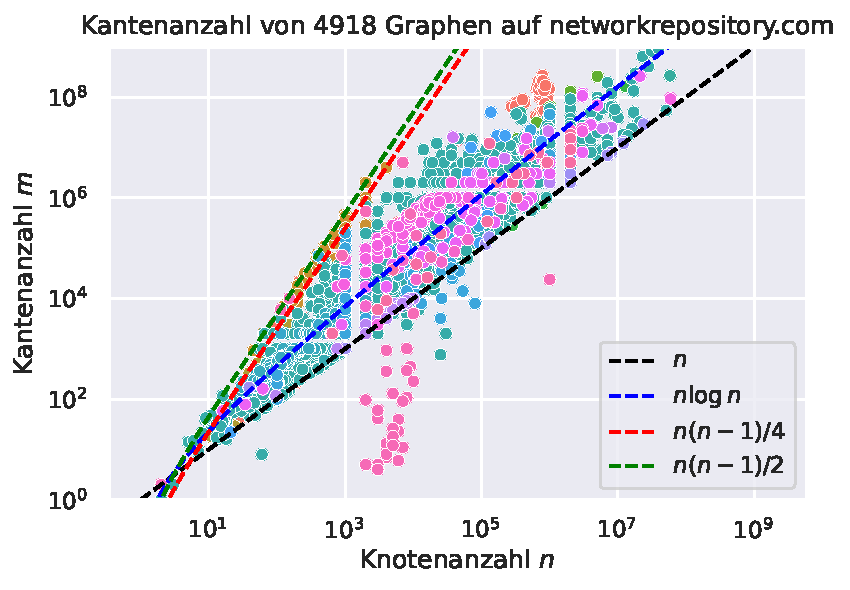
\includegraphics[width=0.5\textwidth]{data/network-rep-edges.pdf}%
        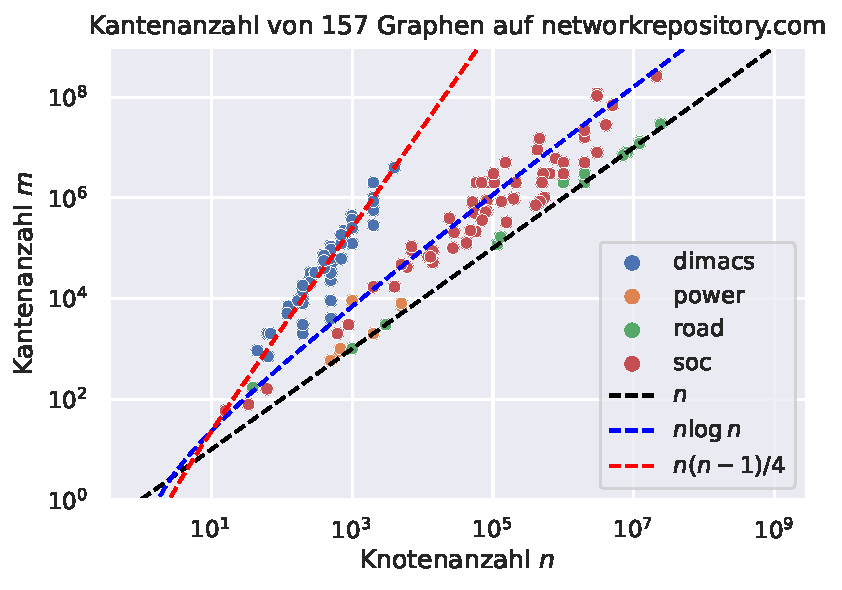
\includegraphics[width=0.5\textwidth]{data/network-rep-edges-thin.pdf}%
    \end{center}
    \caption{
        Die Verteilung der Kantenanzahl in verschiedenen Netzwerken auf~\cite{networkrepository}.
        Die Farben der einzelnen Punkte geben an, aus welchem Bereich die Netzwerke stammen.
    }
    \label{fig:kantenanzahl}
\end{figure}


\begin{observation}
    Sei $G(V,E)$ ein Graph, der zufällig aus $\Gn$ mit $n > 1$ gezogen wurde.
    Dann gilt für gerichtete Graphen $\prob{|E| \ge n^2 / 2} \ge 1/2$ und für ungerichtete Graphen $\prob{|E| \ge \binom{n}{2} / 2} \ge 1/2$.
\end{observation}

\begin{proof}
    Im Folgenden betrachten wir nur gerichtete Graphen; der Beweis läuft analog für ungerichtete Graphen.
    Stellen wir uns einen beliebigen Graphen~$G(V, E)$ vor.
    Dann sei $\bar G(V, \bar E)$ sein Komplement, d.h. für alle möglichen Kanten gilt:
    \begin{equation}
        \forall e \in V\times V\colon \quad\quad e \in \bar E \Leftrightarrow e \notin E
    \end{equation}
    Beobachte, dass es eine Bijektion zwischen allen Graphen in $\mathbb G$ und ihren Komplementen gibt: jeder Graph hat ein eineindeutiges Komplement.
    Per Konstruktion gilt außerdem:
    \begin{eqnarray}
        E \cup \bar E &=& V \times V\\
        \Rightarrow |E| + |\bar E| &\ge& n^2\\
        \Rightarrow \max(|E|, |\bar E|) &\ge& n^2 / 2.
    \end{eqnarray}

    Für jeden Graph~$G$ gilt also, dass entweder $G$ selbst oder sein Komplement~$\bar G$ mindestens $n^2 / 2$ Kanten hat.
    Da wir $G$ und $\bar G$ je mit gleicher Wahrscheinlichkeit ziehen, gilt $\prob{|E| \ge n^2 / 2} \ge 1/2$.
\end{proof}

\section{Kantenanzahl in beobachteten Netzwerken}\label{sec:kanten-in-beobachteten-netzen}
Wie viele Kanten haben echte Netzwerke? Hierzu führen wir ein Experiment durch:
wir nutzen die Datenbank \url{https://networkrepository.com/}, die über 5000 Netzwerke aus unterschiedlichen Bereichen enthält~\cite{networkrepository}.
In \cref{fig:kantenanzahl} zeichnen wir die Kantenanzahl als Funktion der Knotenanzahl.
Zwei Eigenschaften fallen direkt auf:
\begin{enumerate}
    \item Die Kantendichte hängt vom Netzwerktyp ab.
    \item Es sind fast immer deutlich weniger als die Hälfte der Kanten vorhanden.
\end{enumerate}

\subsection{Netzwerktypen haben unterschiedliche Kantendichten}
Betrachten wir die erste Beobachtung genauer, indem wir Straßennetze und Freundschaftsnetze vergleichen.
Wir modellieren ein Straßennetz dadurch, dass Adressen (Häuser, Kreuzung, usw.) als Knoten und Straßen als Kanten dargestellt werden.
Diese Netze \aside{Straßennetze} sind im wesentlichen ein zwei-dimensionales Konstrukt.
Wenn wir Tunnel, Brücken und der gleichen ignorieren, verlaufen Straßen nicht über einander.
Daher erwarten wir, dass die Graphen von Straßennetzen fast planar sind.
Nach dem Eulerischen Polyedersatz erfüllen einfache, \aside{planare Graphen} planare und zusammenhängende Graphen:
\begin{equation}
    |E| \le 3 |V| - 6
\end{equation}
Knoten in einem Straßennetz sollten also im Schnitt höchstens 6 Nachbarn haben.

In \aside{Freundschaftsnetze} sozialen Netzwerken ist die Situation anders ---
stellen wir uns etwa einen Freundschaftsgraphen vor, in dem Knoten die Nutzer eines sozialen Netzwerks sind und Kanten eine Freundschaft anzeigen.
Im Jahr 2014, hatten Facebook-Nutzer im Schnitt mehr als 300 Freunde (mehr dazu später).
Dies ist offensichtlich deutlich mehr als in planaren Graphen möglich wäre.
Ganz ähnlich sieht es mit anderen sozialen Netzen aus: ein durchschnittlicher Erwachsener kennt deutlich mehr als 6 andere Menschen persönlich (oft werden Zahlen zwischen 100 und 300 genannt).

\subsection{Die meisten Netzwerke sind dünn}
In \cref{fig:kantenanzahl} hat nur ein verschwindend geringer Anteil der Netzwerke mindestens die Hälfte aller Kanten (d.h. ist oberhalb der roten Linie).
Wie erklärt sich das?
In der Regel verursacht eine Kante Kosten:
eine Straße muss gebaut werden, eine Freundschaft muss aufrecht erhalten werden (Zeitinvestment), eine Nachricht muss geschrieben werden, etc.
Daher gibt es in den meisten Netzwerken einen gewissen Selektionsdruck, der dazu führt, dass jeder Knoten nur ausgewählte Nachbarn besitzt.
Wir klassifizieren Netzwerktypen, die auffallend viele oder wenig Kanten haben:

\begin{definition}
    Graphen \aside{dünne und dichte Graphen} mit $n$ Knoten und $m$ Kanten heißen \emph{dünn} (engl. sparse), wenn $m = \Oh{n \log n}$ gilt, und \emph{dicht} wenn $m = \Omega(n^2)$.
\end{definition}

\begin{remark}
    Aufgrund der asymptotischen Definition verwendet man \emph{dünn} und \emph{dicht} eher für Graphfamilien (so auch Zufallsgraphen) als für einzelne Instanzen.
    Manche abweichende Definitionen fordern für \emph{dünne} Graphen $m = \Oh{n}$.
    Wir nutzen hier $\Oh{n\log n}$, um soziale Netzwerke mit einzubeziehen.
\end{remark}

\section{Die Zufallsgraphen $\Gnm$ und $\Gnp$}
Das $\Gn$ Modell verfügt über keinen Mechanismus um Kanten auszudünnen.
Wir benötigen also Prozesse, die weniger dichte Graphen erzeugen können ---
am besten parametrisiert, damit wir unterschiedlichen Netzwerktypen Rechnung tragen können.
Im Folgenden betrachten wir zwei solcher Modelle.

Das \Gnm-Modell \aside{Erd\H{o}s-R\'enyi Graphen \Gnm} von P.~Erd\H{o}s und A.~R\'enyi beschreibt die Gleichverteilung über allgemeinen Graphen mit $n$ Knoten und $m$ Kanten, d.h. wir betrachten die Grundmenge
\begin{equation}
    \gGnm = \twoset{G}{G=(V,E) \in \mathbb G(n) \text{ und } |E| = m}.
\end{equation}
Da gleichverteilt gewählt wird, gilt für die Wahrscheinlichkeitsverteilung~{$f\colon \mathbb G \to [0,1]$}
\begin{equation}
    f(G) = \frac{1}{| \gGnm |} \quad \text{ für alle } G \in \gGnm.
\end{equation}

\begin{exercise}
    Berechne $|\gGnm|$ für gerichtete und ungerichtete Graphen.
\end{exercise}

E.~Gilbert \aside{Gilbert-Graphen \Gnp} beschreibt ein ähnliches Modell, das \Gnp-Modell --- das oft fälschlicherweise \glqq Erd\H{o}s-R\'enyi-Modell \grqq{} genannt wird.
Um das Modell zu beschreiben, weichen wir von der bisherigen expliziten Definition der Grundmenge und Verteilung ab.
Stattdessen, spezifizieren wir eine randomisierte Konstruktionsvorschrift:
\begin{enumerate}
    \item Erzeuge $n$ Knoten $V = \{v_1, \ldots, v_n\}$.
    \item Setze $E = \emptyset$.
    \item Für jedes Paar von Knoten $(v_i, v_j)$ führe ein unabhängiges Bernoulli Experiment durch.
          Mit Wahrscheinlichkeit $p$ füge $(v_i, v_j)$ als Kante zu $E$ hinzu.
    \item Gebe den Graphen $G=(V, E)$ zurück.
\end{enumerate}

\noindent
Graphisch kann man sich also \Gnp als Adjazenzmatrix vorstellen, in der die Einträge unabhängig voneinander mit Wahrscheinlichkeit $p$ auf $1$ gesetzt werden:

\begin{center}
    \begin{tikzpicture}
        \node (mat) at (0,0) {
            $\begin{pmatrix}
                    1 & 0 & 1 & 0 & 0 \\
                    0 & 1 & 1 & 0 & 1 \\
                    0 & 1 & 0 & 1 & 0 \\
                    1 & 0 & 1 & 0 & 0 \\
                    1 & 0 & 0 & 0 & 1 \\
                \end{pmatrix}$
        };

        \node[anchor=west, align=left, xshift=4em] (label) at (mat.east) {
            $\begin{cases}1 & \text{mit Wahrscheinlichkeit } $p$ \\
                    0 & \text{mit Wahrscheinlichkeit } 1-p
                \end{cases}$
        };

        \path[draw, thick, bend right, ->] (label.west) to (mat.center);
    \end{tikzpicture}

\end{center}

\begin{exercise}
    Die genannte Konstruktion erzeugt gerichtete Graphen.
    Zeige, wie die Konstruktion so angepasst werden kann, dass gerichtete Graphen ohne Eigenschleifen erzeugt werden.
    Wie verändert sich dann die Adjazenzmatrix?
    Wie verhält es sich mit ungerichteten Graphen?
\end{exercise}

Durch ihre einfache Konstruktion sind beide Zufallsgraphen bis heute sehr verbreitete Modelle in der Netzwerkforschung.
Wir werden jedoch sehen, dass viele Eigenschaften von echten Netzwerken auch von \Gnp oder \Gnm-Graphen nicht beschrieben werden können.

\subsection{Anzahl von Kanten in \Gnp}
Während bei \Gnm Graphen die Anzahl der Kanten durch den Parameter~$m$ fixiert ist, ist $|E|$ bei \Gnp Graphen eine Zufallsvariable.

\begin{lemma}\label{lemma:erwartete_kanten_in_gnp}
    Die \aside{Erwartete Kantenanzahl $\expv{|E|}$ in \Gnp} erwartete Kantenanzahl~$m$ in einem gerichteten \Gnp Graphen ist \begin{equation*} \expv{m} = p n^2. \qedhere \end{equation*}
\end{lemma}

\begin{proof}
    Fixiere einen Graphen~$G=(V,E)$ aus \Gnp.
    Für jede Kante $(u,v)$ definiere die Indikatorvariable $I_{u,v}$, die anzeigt, ob die Kante $(u,v) \in E$ enthalten ist:
    \begin{equation}
        I_{u,v} = \begin{cases}
            1 & \text{ falls } (u,v) \in E \\
            0 & \text{ sonst }
        \end{cases}
    \end{equation}

    \noindent Somit folgt Anzahl der Kanten~$m$ in $G$ als Summe über die Indikatorvariablen
    \begin{equation}
        |E| = \sum_{u,v \in V} I_{u,v} = \left(\sum_{(u,v) \not\in E} 0 \right) +  \left(\sum_{(u,v) \in E} 1\right).
    \end{equation}

    \noindent Per Definition von \Gnp gilt $\prob{I_{u,v} {=} 1} = p$ und $\prob{I_{u,v} {=} 0} = 1-p$.
    Somit folgt für den Erwartungswert jeder Indikatorvariable
    \begin{equation}
        \expv{I_{u,v}} = 1 \cdot p + 0 \cdot (1-p) = p \quad \text{unabhängig für alle } u, v \in V.
    \end{equation}

    \noindent Durch die Linearität des Erwartungswertes folgt schließlich
    \begin{equation}
        \expv{|E|} = \sum_{u,v \in V} \expv{I_{u,v}} = \sum_{u,v \in V} p = p n^2. \qedhere
    \end{equation}
\end{proof}

\begin{exercise}
    Zeige, dass die erwartete Anzahl an Kanten in einem ungerichteten \Gnp Graphen $\expv{|E|} = \binom{n}{2} p = p n(n-1)/2$ beträgt.
\end{exercise}

\begin{exercise}
    Zeige, dass $\Gn = \mathcal G(n, 1/2)$.
\end{exercise}

\bigskip

Wie wir am Beweis von \cref{lemma:erwartete_kanten_in_gnp} sehen, ergibt sich die Kantenanzahl~$m$ als Summe von unabhängigen Bernoulli Zufallsvariablen;
sie ist also selbst eine Zufallsvariable und binomial verteilt.
Da uns die Binomialverteilung regelmäßig begegnen wird, wollen wir uns diese kurz in Erinnerung rufen.
\begin{definition}
    Die \aside{Binomialverteilung.} Binomialverteilung $B_{N, p}(k)$ beschreibt die Wahrscheinlichkeit, dass bei $N$~unabhängigen Bernoulli Experimenten mit Wahrscheinlichkeit $p$ genau $k$ Experimente erfolgreich sind.
    Es gilt \aside{\ \\ \ \\ \ \\ Binomialkoeffizient $\binom{n}{k} = \frac{n!}{(n-k)!k!}$}
    \begin{eqnarray*}
        \prob{B_{N,p} {=} k} &=& \binom{N}{k} p^k (1-p)^{N-k} \\
        \expv{B_{N,p}} &=& Np \\
        \varv{B_{N,p}} &=& Np(1-p),
    \end{eqnarray*}
    wobei $\expv{B_{N,p}}$ und $\varv{B_{N,p}}$ den Erwartungswert und die Varianz der Binomialverteilung beschreiben.
\end{definition}

Die Standardabweichung $\sigma = \sqrt{\varv{B_{N,p}}} \le \sqrt{\expv{B_{N,p}}}$ ist also relativ klein.
Wir können daher davon ausgehen, dass für hinreichend großes $N$ die Binomialverteilung recht stark um ihren Erwartungswert $Np$ konzentriert ist.
Daher sagen wir, dass \Gnm und \Gnp mit $p=m/n^2$ asymptotisch (d.h. für $n \to \infty$) äquivalent sind.
Häufig ist es jedoch einfacher \Gnp Graphen zu analysieren, da ---im Gegensatz zu \Gnm Graphen--- alle Kanten unabhängig gezogen werden.

\section{Effizientes Ziehen von \Gnp Graphen}
Zufallsgraphen sind nicht nur in der theoretischen Analysen von Prozessen und Algorithmen nützlich, sondern auch für empirische Untersuchungen.
Nehmen wir etwa an, dass wir einen Algorithmus implementiert haben und dessen Geschwindigkeit oder Qualität vermessen möchten.
Dann können Zufallsgraphen unter anderem aus folgenden Gründen nützlich sein:
\begin{itemize}
    \item Wenn die Generatorsoftware vorhanden ist, können wir synthetische Instanzen in quasi unbeschränkter Menge generieren.
    \item Parametrisierte Generatoren erlauben den Einfluss gewisser Eigenschaften detailliert zu analysieren; z.B. Skalierungsexperimente.
    \item Beobachtete Graphen haben oft \glqq Rauschen\grqq, d.h. nicht verstandene oder insignifikante Strukturen, die Messungen verfälschen können.
          Zufallsgraphen, hingegen, haben i.d.R. eine gut verstandene Struktur, die es uns oft ermöglicht vor dem Testen Hypothesen aufzustellen.
    \item Einige Generatoren können anhand eines fixierten Startzustands (Random-Seed) dieselben Graphen wiederholt erzeugen.
          Wir müssen also die Eingaben nicht speichern/transferieren und können dennoch reproduzierbare Experimente durchführen.
\end{itemize}

\noindent Da in verschiedenen wissenschaftlichen Communities der Begriff \glqq Generator\grqq{} unterschiedlich benutzt wird, hier noch eine Definition:
\begin{definition}
    Ein \aside{Graphgenerator} Graphgenerator ist ein Algorithmus, der einen Graphen aus einem Netzwerkmodell erzeugt.
    Dieser respektiert die Verteilung des zugrundeliegenden Modells.
\end{definition}

\subsection{Ein naiver Ansatz}
Betrachten wir folgenden Graphgenerator für \Gnp Graphen, der im wesentlichen eine 1:1 Implementierung der Definition von \Gnp ist:

\begin{algorithm}[H]
    \KwIn{Anzahl der Knoten~$n$ und Verbindungswahrscheinlichkeit~$p$}
    \KwOut{Adjazenzmatrix eines zufälligen Graphs $G \follows \Gnp$}
    Allokiere eine Matrix $A[1..n, 1..n]$\;
    \For{$1 \le i \le n$}{
        \For{$1 \le j \le n$}{
            Setze $A[i,j] \gets \begin{cases}
                    0 & \text{mit Wahrscheinlichkeit } 1-p \\
                    1 & \text{mit Wahrscheinlichkeit } p
                \end{cases}$\;
        }
    }
    Gebe $A$ zurück
    \caption{Naiver Graphgenerator für \Gnp Graphen}
    \label{alg:naive-gnp}
\end{algorithm}

Um \aside{Annahme: aus einfachen Verteilungen kann in kostanter Zeit gezogen werden.} die Laufzeit dieses Algorithmus bestimmen zu können, treffen wir in dieser Veranstaltung folgende Annahme.
Wir können unter anderem aus folgenden Zufallsverteilungen in konstanter Zeit ziehen:
\begin{itemize}
    \item Ganzzahlig uniform aus $[a, b]$ für $a, b \in \mathbb{Z}$.
    \item Gleitkommazahl uniform aus $[a, b]$ für $a, b \in \mathbb{R}$.
    \item Bernoulli (folgt aus vorherigem Punkt)
    \item Binomial, Geometrisch (siehe \cref{{sec:inversionsmethode}}), Hypergeometrisch, Poisson
\end{itemize}

Tatsächlich können die meisten dieser Verteilungen nur in \emph{erwartet} konstanter Zeit gezogen werden, praktisch sind die Fluktuationen jedoch so klein, dass wir sie vernachlässigen können.
Das erlaubt es uns auf die Eigenschaften der Graphgeneratoren zu konzentrieren.

\begin{lemma}
    \label{lem:naive-gnp}
    Der Algorithmus \ref{alg:naive-gnp} erzeugt einen \Gnp Graphen in $\Theta(n^2)$ Zeit.
\end{lemma}

\begin{exercise}
    Beweise das Lemma.
\end{exercise}

Nun könnte man argumentieren, dass dieser naive Algorithmus bereits optimal ist:
Die Ausgabe hat Größe $\Theta(n^2)$ und somit wir benötigen $\Omega(n^2)$ Zeit, um die Ausgabe zu erzeugen.
Außerdem hat ein Graph mit $p=\Omega(1)$ erwartete $\Theta(n^2)$ Kanten, was wiederum die Laufzeit von unten beschränkt.

Diese Worst-Case Schranken passen jedoch nicht zu unserer Beobachtung in \cref{sec:kanten-in-beobachteten-netzen}, dass Graphen in der freien Wildbahn meist dünn sind.
Es wäre schön, wenn wir diese Graphen schneller erzeugen könnten, jedoch ist \cref{alg:naive-gnp} für alle $p$ gleich \glqq schnell\grqq.
Hier \aside{ausgabesensitive Algorithmen} helfen \emph{ausgabesensitive Algorithmen} (output-sensitive algorithm), deren Laufzeit maßgeblich durch die Größe der Ausgabe bestimmt wird;
die meisten Generatoren, die wir betrachten werden, fallen genau in diese Kategorie.

Ausgabesensitive \aside{Kantenlisten} Algorithmen müssen jedoch eine Ausgabedatenstruktur nutzen, die sich an die Größe anpasst.
Eine Matrix hat immer dieselbe Größe unabhängig davon, wie viele Einsen (Kanten) vorhanden sind.
Wir werden im Folgenden fast immer eine Kantenliste annehmen, die nur $\Oh{1}$ Speicherworte pro Kante benötigt.

\subsection{Ziehen mit zufälligen Sprüngen}\label{subsec:gnp_zufaellige_spruenge}
Wie können wir nun \cref{alg:naive-gnp} verändern, so dass er ---analog zu Kantenlisten--- keine Arbeit für Nichtkanten verrichtet?
Idee: Wir müssen diese einfach überspringen!
Aber woher wissen wir wo \glqq Nullen\grqq{} gezogen werden, bzw. wie viele Nullen müssen wir überspringen?
Zählen können wir sie nicht ohne wieder direkt quadratische Arbeit zu verrichten.

Ganz \aside{Effizientes Ziehen durch Überspringen von Nullen} einfach: wir fragen uns wie viele Nullen~$\ell$ \cref{alg:naive-gnp} gesetzt hätte und überspringen diese.
Zwischen diese zufälligen Sprünge setzen wir dann die Einsen ein.
Wenn wir nun $\ell$ aus einer geeigneten Verteilung ziehen, haben wir zwei unterschiedliche Zufallsprozesse, deren Ausgabe aber nicht unterscheidbar ist.
Generalisierungen dieser Methode werden uns noch häufiger begegnen.

Zur \aside{Statt $n \times n$ Matrix, nehmen wir einen $n^2$ Vektor an} Vereinfachung stellen wir uns die Adjazenzmatrix~$A = (a_{ij})_{ij}$ als einen Vektor~$B = (b_k)_k$ vor, der dadurch entsteht, dass wir die Zeilen hinter einander anfügen (row-major layout).
Eintrag $a_{ij}$ wird also mit $b_{(i-1)n + j}$ identifiziert.
Dann besteht unsere Aufgabe darin genau alle $b_k$ zu finden, die den Wert $1$ haben.

\begin{equation}
    \Big(\quad \cdots \overbrace{1}^{b_k} \ \underbrace{0 \ \ 0\ \ 0 \ \cdots\ \ 0\ \ 0\ \ 0}_{\text{$\ell$ zusammenhängende Nullen}}\  \overbrace{1}^{b_{k + 1+ \ell}} \cdots \quad \Big)
\end{equation}

\noindent
Sei $X$ die \aside{Anzahl Nullen $X$ ist geometrisch verteilt} Zufallsvariable, welche die Anzahl der Nullen nach einer Eins modelliert.
\begin{eqnarray}
    \prob{X = 0} &=& \prob{\text{Nächster Versuch: 1}} = p \\
    \prob{X = 1} &=& \prob{\text{Nächster Versuch: 0, dann 1}} = (1 - p)p \\
    \prob{X = 2} &=& \prob{\text{Nächster Versuch: 0, dann 0, dann 1}} = (1 - p)^2 p \\
    &\vdots& \\
    \prob{X = \ell} &=& (1 - p)^\ell p
\end{eqnarray}

\noindent Die Zufallsvariable ist also \emph{geometrisch verteilt} mit Parameter $p$.
Es ergibt sich also der folgende einfache Algorithmus:

\begin{algorithm}[H]
    \KwIn{Anzahl der Knoten~$n$ und Verbindungswahrscheinlichkeit~$p$}
    \KwOut{Kantenliste $E$ eines zufälligen Graphs $G \follows \Gnp$}
    Initialisiere eine leere Kantenliste $E$\;
    $k \gets -1$\;
    \While{true}{
        $\ell \gets \text{ziehe die Sprungweite aus einer geometrischen Verteilung mit Parameter $p$}$\;
        $k \gets k + \ell + 1$\;

        \If{$k < n^2$}{
            $(i, j) \gets (\lfloor k / n \rfloor$, \ k \text{ mod } n)\;
            $E \gets E \cup \{(i+1, j+1)\}$\;
        } \Else {
            Gebe $E$ zurück und beende\;
        }
    }
    \caption{Generator für \Gnp Graphen mit zufällige Sprüngen}
    \label{alg:linear-gnp}
\end{algorithm}

\begin{lemma}
    \label{lem:linear-gnp}
    Algorithmus \ref{alg:linear-gnp} erzeugt Graph $G(V, E) \follows \Gnp$ in $\Theta(|E|)$ Zeit.
\end{lemma}

\begin{exercise}
    Beweise das Lemma.
\end{exercise}
\begin{exercise}
    Passe \cref{alg:linear-gnp} für ungerichtete Graphen an.
\end{exercise}

Jetzt müssen wir nur noch herausfinden, wie wir geometrische Sprünge effizient ziehen können.
Hierzu kommt meist die Inversionsmethode zum Einsatz.

\subsection{Inversionsmethode: Ziehen aus der geometrischen Verteilung}
\label{sec:inversionsmethode}

\begin{figure}[t]
    \begin{center}
        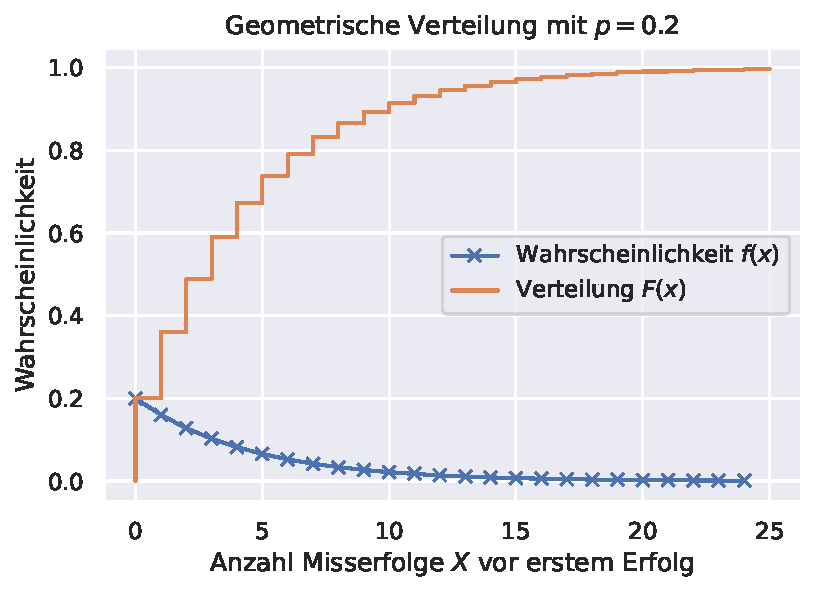
\includegraphics[width=0.5\textwidth]{data/geometric-distr.pdf}%
        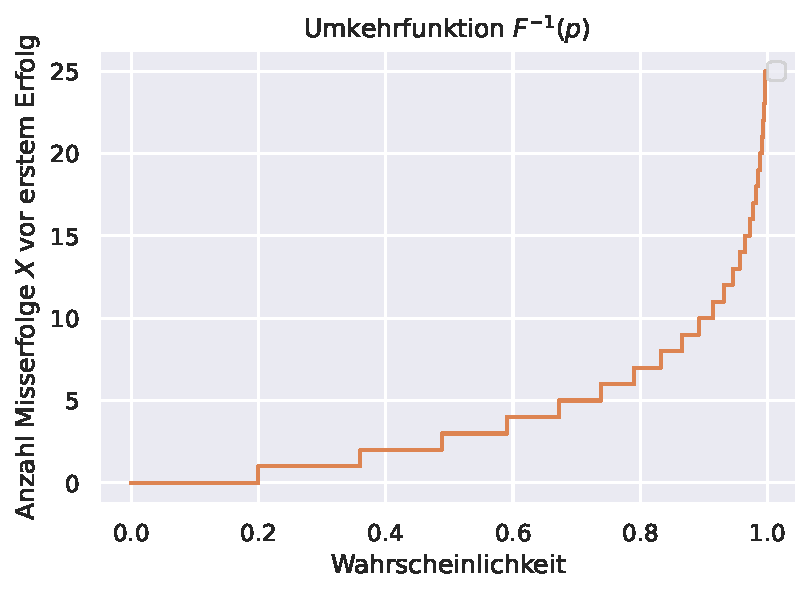
\includegraphics[width=0.5\textwidth]{data/geometric-distr-inv.pdf}
    \end{center}

    \caption{
        Wahrscheinlichkeitsverteilung und kumulative Verteilungsfunktion einer geometrischen Verteilung mit Parameter $p = 0.2$ (links).
        Die rechte Abbildung zeigt die \glqq Umkehrfunktion\grqq{} $F^{-1}(p)$ der kumulativen Verteilungsfunktion $F(x)$.
    }
    \label{fig:geometric-distr}
\end{figure}

Die \aside{Inversionsmethode: effizientes Ziehen falls Umkehrfunktion bekannt} Inversionsmethode (inversion transform method) ist ein allgemeines Verfahren, um eine uniforme Zufallsvariable in eine andere Verteilung zu übersetzen.
Wir betrachten die Methode hier am Beispiel der geometrischen Verteilung.
In \cref{fig:geometric-distr} ist die Wahrscheinlichkeitsverteilung $f(\ell)$ und die kumulative Verteilungsfunktion $F(\ell)$ einer geometrischen Verteilung mit Parameter $p = 0.2$ gezeigt.
%
%Da $f(\ell)$ ist eine Wahrscheinlichkeitsverteilung ist, muss $\sum_{\ell=0}^{\infty} f(\ell) = 1$ gelten.
Betrachten wir die konkreten ersten drei Werte der Funktionen:

\begin{center}
    \begin{tabular}{l|p{0.2\textwidth}p{0.25\textwidth}p{0.35\textwidth}}
                  & $\ell = 0$ & $\ell = 1$              & $\ell = 2$                              \\\hline\hline
        $f(\ell)$ & $p =0.2$   & $(1 {-} p)p = 0.16$     & $(1 {-} p)^2p = 0.128$                  \\
        $F(\ell)$ & $p =0.2$   & $p{+}(1 {-} p)p = 0.36$ & $p{+}(1 {-} p)p{+}(1 {-} p)^2p = 0.488$
    \end{tabular}
\end{center}
\vspace{1em}

Ein Generator sollte also z.B. den Wert $0$ mit Wahrscheinlichkeit 20\,\% ausgeben.
Da wir einen deterministischen Algorithmus konstruieren möchten, brauchen wir eine Quelle für den Zufall:
wir erwarten eine uniforme Zufallsvariable $U \in [0, 1)$ als Eingabe.
Wir können also z.B. prüfen:
\begin{itemize}
    \item Wenn $U < 0.2$ ist, dann gebe den Wert $0$ zurück.
          Da $U$ uniform verteilt ist, ist die Wahrscheinlichkeit für $U < 0.2$ genau $0.2$.

    \item Falls nicht prüfen wir, ob $U < 0.36 = f(0) + f(1) = F(1)$ ist. Falls ja, geben wir den Wert $1$ zurück.
          Da $U$ uniform verteilt ist, wir aber wissen, dass $U$ nicht kleiner als $0.2$ ist, ist die Wahrscheinlichkeit $\prob{U < 0.36 | U > 0.2} = 0.16 = f(1)$.

    \item Diesen Prozess setzen wir fort, bis wir das passende Intervall gefunden haben.
\end{itemize}

Die graphische Interpretation ist also die folgende:
In \cref{fig:geometric-distr} (rechts) ist die Umkehrfunktion~$F^{-1}(p)$ der kumulativen Verteilungsfunktion $F(x)$ gezeigt.
Wir werfen nun mittels der zufälligen Eingabe $U$ einen Punkt auf der $x$-Achse und schauen, welchen Wert $F^{-1}(U)$ hat --- dies ist unsere Ausgabe.

Im folgenden Theorem wird die Inversionsmethode formalisiert, wobei wir vereinfachend einige Annahmen treffen.
Die Methode lässt sich aber auch auf andere $\Omega$ (inklusive kontinuierliche) und nicht streng monotone $F(x)$ verallgemeinern.

\begin{theorem}
    Sei $X \in \Omega$ eine diskrete Zufallsvariable und $f(x)$ und $F(x)$ ihre Wahrscheinlichkeitsverteilung sowie die kumulative Verteilungsfunktion.
    Vereinfachend sei $\Omega$ total geordnet und $F(x)$ streng monoton steigend.
    Dann existiert die Umkehrfunktion $F^{-1}(x)$ mit $F^{-1}(F(x)) = x$.
    Sei $U$ eine uniforme Zufallsvariable aus $[0, 1)$.
    Dann ist $X' = F^{-1}(U)$ eine Zufallsvariable mit der Wahrscheinlichkeitsverteilung $f(x)$.
\end{theorem}

\begin{proof}
    \noindent Da $F$ streng monoton ist, existiert die Umkehrfunktion $F^{-1}$ und es gilt:
    \begin{equation}\label{eq:inverse-apply-inverse}
        F(x) = p
        \quad\Leftrightarrow\quad F^{-1}(F(x)) = F^{-1}(p)
        \quad\Leftrightarrow\quad x = F^{-1}(p)
    \end{equation}

    \noindent Daraus folgt dann direkt:
    \begin{eqnarray}
        \prob{X' \le x} &\stackrel{\text{Inv. Method}} = & \prob{F^{-1}(U) \le x} \\
        &\stackrel{(\ref{eq:inverse-apply-inverse})}{=}& \prob{U \le F(x)} \\
        &\stackrel{\prob{U < z} = z \forall z \in [0, 1]}=& F(x) \\
        &\stackrel{\text{Def.} F(X)}=& \prob{X \le x} \hspace{5em}\hfill \qedhere
    \end{eqnarray}
\end{proof}

\bigskip
\bigskip

\begin{figure}
    \begin{center}
        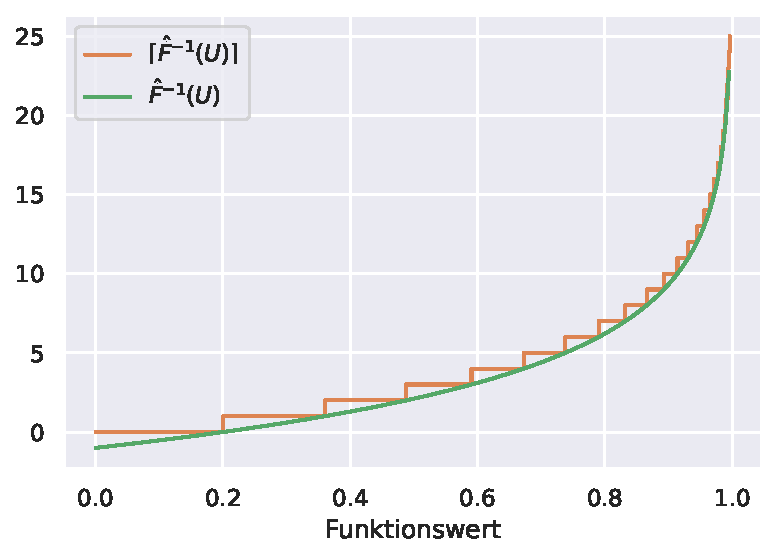
\includegraphics[width=0.5\textwidth]{data/geometric-distr-inv_hat.pdf}
    \end{center}
    \caption{Die in \cref{eq:inverse-hat} berechnet Umkehrfunktion $\hat F^{-1}(U)$}

\end{figure}

Zurück \aside{Inversionsmethode für geometrische Verteilung} zur geometrischen Verteilung mit $f(\ell) = (1-p)^\ell p$.
ObdA sei $0 < p < 1$ (da $X$ sonst eine Konstante ist).
Die kumulative Verteilungsfunktion lautet
\begin{equation}
    F(\ell)
    \ =\ p \sum_{i=0}^\ell (1-p)^\ell
    \ \stackrel{(*)}{=} \ p \frac{1 - (1-p)^{\ell+1}}{\underbrace{1 - (1-p)}_{=p}}
    \ = \ 1 - (1-p)^{\ell+1},
\end{equation}
wobei wir in $(*)$ die geschlossene Form der $\ell$-ten Partialsumme der geometrischen Reihe nutzen $\sum_{i=0}^\ell x^\ell = (1 - x^{\ell+1})/(1 - x)$.
Nun berechnen die Umkehrfunktion $\hat F^{-1}(U) = \ell$ indem wir $F(\ell) = U$ setzen und nach $U$ umformen.
Hierbei nehmen wir zunächst an, dass die Funktion stetig wäre (daher schreiben wir $\hat F ^{-1}$ statt $F^{-1}$):
\begin{eqnarray}
    U &=& F(\ell) = 1 - (1-p)^{\ell+1} \\
    \Leftrightarrow (1-p)^{\ell+1} &=& 1 - U \\
    \Leftrightarrow  (\ell+1) \log(1-p)  &=& \log(1 - U) \\
    \Leftrightarrow  \hat F^{-1}(U) := \log_{1-p}(1 - U) - 1 &=& \ell \label{eq:inverse-hat}
\end{eqnarray}

Schließlich erhalten wir $F^{-1}(U) = \lceil \hat F^{-1} (U) \rceil$ durch Aufrunden der gerade berechneten Funktion.
Zusammenfassen erzeugt \cref{alg:sample-geometric} eine geometrische Zufallsvariable $X$ mit Parameter $p$ in Zeit $\Oh{1}$:

\begin{algorithm}[H]
    \If{p=0}{Gebe $\infty$ zurück}
    \ElseIf{p=1}{Gebe $0$ zurück}
    \Else{$U \gets \text{ziehen uniform aus $[0, 1)$}$\;
    Gebe $\lceil \log_{1-p}(1 - U) - 1\rceil$ zurück.}
    \caption{Ziehen einer geometrischen Zufallsvariable}
    \label{alg:sample-geometric}
\end{algorithm}

\bigskip
\bigskip

\section{Effizientes Ziehen von \Gnm Graphen}
Trotz der strukturellen Ähnlichkeiten zwischen \Gnp und \Gnm Graphen unterscheiden sich ihre Generatoren signifikant.
Grund hierfür ist, dass während \Gnp \emph{in Erwartung} $n^2p$ Kanten erzeugen, müssen wir für \Gnm Generatoren sicherstellen, dass exakt $m$ zufällige Kanten produziert werden.

Ähnlich wie zuvor, reduzieren wir das Ziehen der richtigen Position von \emph{Einsen} in der Adjazenzmatrix auf den eindimensionalen Fall.
Im Folgenden werden wir also folgendes äquivalentes Problem lösen:
Ziehe uniform ohne Zurücklegen $k$ Elemente aus einer Menge $S = \set{s_1, \ldots, s_N}$ mit $|S| = N > k$.

\subsection{Reservoir Sampling}
Reservoir Sampling ist eine allgemeine Technik, die es uns erlaubt $k$ Elemente aus einem Datenstrom zu ziehen.
Hierbei müssen wir anfangs \emph{nicht} wissen, wie viele Elemente insgesamt im Strom sind.\footnote{
    Ein praktischer Anwendungsfall sind z.B. Iteratoren oder Generatoren, die in vielen Programmiersprachen genutzt werden.
    In Rust ist z.B. \texttt{rand::IteratorRandom::choose\_multiple} mittels Reservoir Sampling implementiert.
}
Im konkreten Fall besteht der Datenstrom also aus allen $s_i$ in beliebiger Reihenfolge.
Vereinfachend können wir also annehmen, dass der Strom mindestens $k$ Elemente enthält.

\begin{algorithm}[H]
    \KwIn{Eingabe: Datenstrom~$S$, Stichprobengröße~$k$}
    \KwOut{Array $R[1..k]$ mit $k$ zufällig ausgewählten Elementen}

    Initialisiere ein anfangs leeres Array $R$ mit Kapazität $k$\;

    \While{$|R| < k$}{
        $x \gets \text{nächstes Element aus $S$}$\;
        Füge $x$ an $R$ an\;
    }

    Setze $i = k$\;
    \While{$S$ nicht leer}{
        $x \gets \text{nächstes Element aus $S$}$\;
        $i \gets i + 1$\;
        $j \gets \text{ziehe uniform aus $[1, i]$}$\;
        \If{$j \le k$}{
            Ersetze $R[j] \gets x$\;
        }
    }

    Gebe $R$ zurück

    \caption{Reservoir Sampling}
    \label{algo:reservoir-sampling}
\end{algorithm}

\bigskip
\bigskip

\noindent
In \cref{thm:reservoir-sampling} zeigen wir die Korrektheit von \cref{algo:reservoir-sampling} für nur $k = 1$:
\begin{theorem}\label{thm:reservoir-sampling}
    Für $k=1$ liefert \cref{algo:reservoir-sampling} liefert ein uniform gewähltes Element $x\in S$.
\end{theorem}

\begin{proof}
    Sei $N$ die Länge des Stroms (ist dem Algorithmus nicht bekannt).
    Seien zudem $s_1, \ldots, s_N$ die Elemente in der Reihenfolge, in der sie aus dem Strom gelesen werden;
    oBdA gelte $s_i = s_j \ \Leftrightarrow\ i = j$ (d.h. alle Elemente sind unterschiedlich; falls nicht, können wir die Tupel $(s_i, i)$ betrachten).

    Sei $R$ die Zufallsvariable, welche die Ausgabe des Algorithmus modelliert.
    Dann ist zu zeigen, dass $\prob{R = s_i} = 1 / N$ für alle $1 \le i \le N$.
    \begin{eqnarray}
        \prob{R = s_i} &=& \prob{\text{$s_i$ wird in Runde~$i$ gewählt}} \cdot \prob{\text{$s_i$ wird nicht ersetzt}} \\
        &=& \frac{1}{i} \cdot \underbrace{\prod_{j=i+1}^N \frac{j-1}{j}}_{\text{Teleskop-Produkt}}
        = \frac{1}{i} \cdot \frac{i}{N} = \frac{1}{N}
    \end{eqnarray}

    \noindent Insbesondere gilt also, dass $\prob{R = s_i} = 1/N$ unabhängig von $i$ oder $s_i$ ist.
\end{proof}

\begin{exercise}
    Zeige die Korrektheit von \cref{algo:reservoir-sampling} indem du den Beweis von \cref{thm:reservoir-sampling} auf $k \ge 1$ verallgemeinerst.
    Dies lässt sich etwa über Induktion über die Datenstromlänge $|S|$ erreichen.
\end{exercise}

Wir können also \Gnm Graphen mittels Reservoir Sampling erzeugen.
Allerdings entspricht jede potentielle Kante einem Element in $S = V \times V$, für das wir je $\Theta(1)$ Arbeit verrichten müssen;
somit folgt eine Gesamtlaufzeit von $\Theta(n^2)$.

\subsection{Ziehen mit Lookups}
Im Folgenden skizzieren wir einen alternativen Ansatz um $k$~Elemente ohne Zurücklegen aus dem Universum~$S$ zu ziehen; dieser basiert auf \cite{batagelj2005efficient}.
Dieser nutzt das Grundgerüst in~\cref{algo:basis-ziehen-ohne-zuruecklegen}, das wir um einige Details erweitern müssen, um eine praktisch schnelle Implementierung zu erreichen:

\begin{algorithm}[H]
    \KwIn{Eingabe: Universum~$S$, Stichprobengröße~$k$}
    \KwOut{Menge $R$ mit $k$ zufällig ausgewählten Elementen}

    Initialisiere $R = \emptyset$\;

    \While{$|R| < k$}{
        $x \gets $ zufälliges Element aus $S$\;
        \If{$x \not\in R$}{
            $R \gets R \cup \set{x}$
        }
    }

    Gebe $R$ zurück

    \caption{Basisalgorithmus für Ziehen ohne Zurücklegen}
    \label{algo:basis-ziehen-ohne-zuruecklegen}
\end{algorithm}

\bigskip

Wir messen die Geschwindigkeit des Algorithmus zunächst nur indirekt, indem wir die Anzahl der Iterationen der \texttt{while}-Schleife zählen:

\begin{lemma}\label{lemma:basis-ziehen-ohne-zuruecklegen-versuche}
    \Cref{algo:basis-ziehen-ohne-zuruecklegen} verwendet in Erwartung $N \log(N/(N-k+1)) + \Oh{1}$ Versuche (Iterationen der \texttt{while}-Schleife) um aus $S$ mit $|S| = N$ exakt $1 \le k < N$ Elemente zu ziehen.
\end{lemma}

\begin{proof}
    Der Algorithmus baut $R$ inkrementell auf: wir beginnen mit $|R| = 0$ und fügen dann schrittweise je ein Element hinzu.
    Sei $X$ eine Zufallsvariable, die beschriebt, wie viele Iterationen der Algorithmus benötigt um $R$ zu erzeugen.
    Ferner seien $X_1, \ldots, X_k$ Zufallsvariablen, wobei $X_i$ beschriebt, wie viele Versuche benötigt werden um das $i$-te Elemente zu finden (d.h. um $R$ von $|R| = i - 1$ auf  $|R| = i$ zu heben).
    Per Konstruktion gilt $X = \sum_{i=1}^k X_i$ und aufgrund der Linearität des Erwartungswertes folgt

    \begin{equation}
        \expv{X} = \expv{\sum_{i=1}^k X_i} = \sum_{i=1}^k \expv{X_i}. \label{eq:basis-ziehen-ohne-zuruecklegen_expvX}
    \end{equation}

    Wir können also zunächst die Erwartungswerte $\expv{X_i}$ isoliert betrachten.
    Unmittelbar bevor wir das $i$-te Element ziehen, haben wir $i-1$ Elemente bereits bestimmt, d.h. $|R| = i - 1$.
    Mit Wahrscheinlichkeit $q_i = (i-1) / N$ erwischen wir also ein bereits gezogenes Element und versuchen es erneut.
    Mit Wahrscheinlichkeit $p_i = 1 - q_i = (N - (i - 1)) / N$ ziehen wir aber ein Element, dass noch nicht Teil von $R$ ist.
    Es gilt also

    \begin{align*}
        \prob{X_i = 1}            & = p_i                  \\
        \prob{X_i = 2}            & = (1 -p_i) p_i         \\
        \vdots         \quad\quad & = \quad\quad \vdots    \\
        \prob{X_i = 1 + \ell}     & = (1- p_i)^{\ell} p_i.
    \end{align*}

    Die Zufallsvariable $X_i - 1$ ist also geometrisch verteilt mit Erfolgswahrscheinlichkeit~$p_i$.
    Es gilt daher $\expv{X_i} = 1 / p_i = N / (N - i + 1)$. Durch Einsetzen in \cref{eq:basis-ziehen-ohne-zuruecklegen_expvX} erhalten wir:
    \begin{align}
        \expv{X} & = \sum_{i=1}^k \frac{N}{N-(i-1)} = \sum_{i=0}^{k-1} \frac{N}{N - i}                                      \\
                 & = N \sum_{i=N-k+1}^N \frac{1}{i}                                                                         \\
                 & = N \left[ \left( \sum_{i=1}^N \frac{1}{i} \right) - \left( \sum_{i=1}^{N-k} \frac{1}{i} \right) \right] \\
                 & = N \left[ H_N - H_{N-k} \right]
    \end{align}

    Im letzten Schritt nutzen wir die Definition $H_t = \sum_{i=1}^t 1/i$, also die $t$-te Partialsumme der Harmonischen Reihe.
    Es gilt, dass $H_t = \ln t + \gamma + 1/(2t) + \varepsilon_t$, wobei $\gamma \approx 0.5772$ die Euler–Mascheroni Konstante ist und $0 \le \varepsilon_t \le N^{-2}/8$ ein verschwindender Fehlerterm ist.
    Es folgt also:
    \begin{align}
        \expv{X} & = N \left[ H_N - H_{N-k} \right]                      \\
                 & \le N \left[ \ln N - \ln (N - k + 1) \right] + \Oh{1} \\
                 & = N \ln \frac{N}{N - k + 1} + \Oh{1}
    \end{align}
\end{proof}

\noindent
\begin{figure}
    \begin{center}
        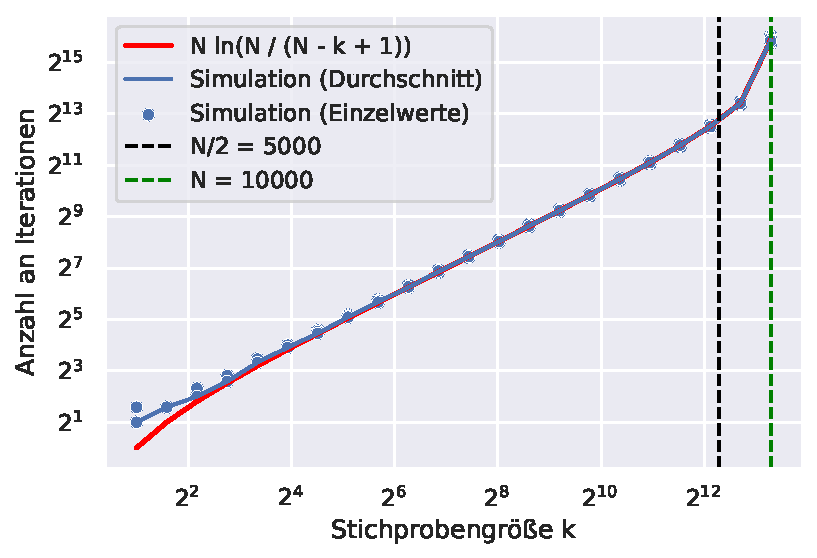
\includegraphics[width=0.5\textwidth]{data/gnm_iterationen.pdf}%
        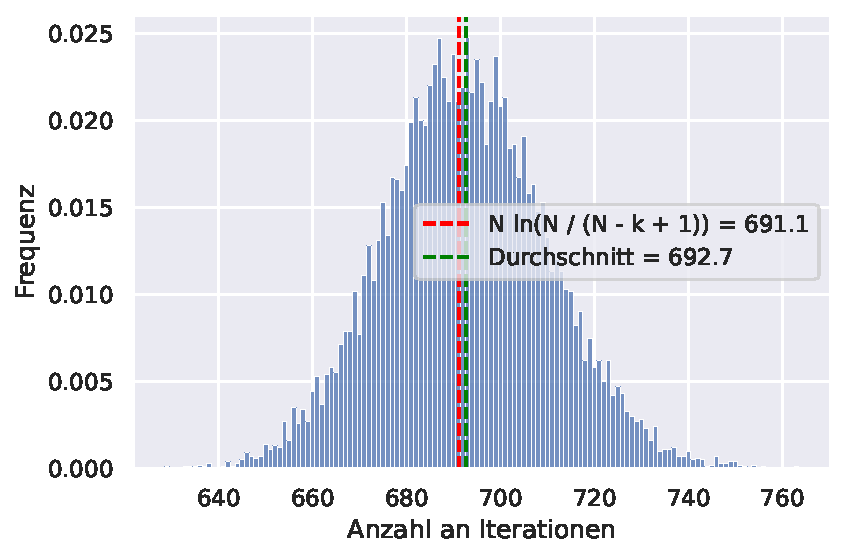
\includegraphics[width=0.5\textwidth]{data/gnm_iterationen_hist.pdf}
    \end{center}
    \caption{Simulation von \cref{algo:basis-ziehen-ohne-zuruecklegen} (ohne Komplementbildung).
        \textbf{Links}: $N=10\,000$ und $2 \le k \le 3N/4$; für jeden Parameter wurden 1\,000 unabhängige Simulationen ausgeführt.
        \textbf{Rechts}: $N=1\,000$, $k = N/2$. Es wurden 10\,000 unabhängige Simulationen ausgeführt.
    }
    \label{fig:ziehen-ohne-zuruecklegen-iterationen}
\end{figure}

Beobachte, dass die Analyse im Beweis von \cref{lemma:basis-ziehen-ohne-zuruecklegen-versuche} sehr eng ist.
Wie wir in \cref{fig:ziehen-ohne-zuruecklegen-iterationen} sehen, gilt für relativ kleine $N$ schon $\expv{X} \approx N \ln \frac{N}{N - k + 1}$.

\begin{exercise}
    Zeige, dass $N \ln \frac{N}{N - k + 1} = \Oh{k}$ für $k \le N / 2$.
\end{exercise}

\bigskip

\Cref{lemma:basis-ziehen-ohne-zuruecklegen-versuche} besagt, dass \cref{algo:basis-ziehen-ohne-zuruecklegen} für $k \le N / 2$ erwartet $\Oh{k}$ Iterationen ausführt und somit (in Erwartung) optimal ist.
Nur für $k \to N$ wird der $\log$-Faktor asymptotisch relevant, und wir bekommen eine suboptimale Laufzeit von $\Omega(N \log N)$.

Auf \aside{Komplementbildung stellt sicher: $k \ge N /2$} der einen Seite sollte das für \emph{übliche} Graphen kein Problem sein (sie sind dünn und daher $k \ll N$); dennoch lässt sich das Problem einfach vermeiden.
Für $k > N / 2$ können wir zunächst das Komplement~$\bar R$ mit  $| \bar R | = N - k < N/2$ ziehen und dann alle Elemente außer solche in $\bar R$ ausgeben.
Zwar benötigt die Komplementbildung $R = \bar{\bar R}$ während der Ausgabe $\Theta(N)$ Zeit, allerdings hat die Ausgabe ebenfalls Größe $\Omega(N)$, wodurch das asymptotisch optimal bleibt.

\subsection{Konzentration um den Erwartungswert}
Bisher haben wir uns darauf konzentriert Performance \emph{in Erwartung} zu analysieren.
In der Praxis kann das aber manchmal zu wenig sein:
wir stellen uns eine Implementierung vor, die in 99~\% der Fälle in 1\,s durchläuft aber in 1~\% der Ausführungen 101\,s benötigt.
Die durchschnittliche (\qq{erwartete}) Laufzeit wären also 2\,s.
Wenn wir unsere Pipelines darauf auslegen, kann das zu (im schlimmsten Fall kaskadierenden) Timeouts führen.

\Cref{fig:ziehen-ohne-zuruecklegen-iterationen} (rechts) scheint zu zeigen, dass \cref{algo:basis-ziehen-ohne-zuruecklegen} nicht in diese Kategorie fällt.
Unter 10\,000 Ausführung ist die größte Abweichungen vom Mittelwert nur rund 12\,\%.
Um Beobachtungen wie diese zu formalisieren, nutzt man häufig folgende Definition:

\begin{definition}
    Eine \aside{mit hoher Wahrscheinlichkeit} Eigenschaft~$X$ gilt \emph{mit hoher Wahrscheinlichkeit} (with high probability, whp),
    wenn für einen hinreichend großen Parameter $n$ die Gegenwahrscheinlichkeit $\prob{\lnot X} \le 1/n$ nicht übersteigt.
\end{definition}

In anderen Worten: je \qq{größer} unser Problem wird, desto unwahrscheinlicher sind extreme Ausreißer.
In der Regel ist der Parameter aus dem Kontext klar und wird daher in der Literatur oft nicht erwähnt (im folgenden Lemma wäre es $k$):

\begin{lemma}
    \Cref{algo:basis-ziehen-ohne-zuruecklegen} verwendet mit hoher Wahrscheinlichkeit \Oh{k} Iterationen für $k \le N/2$.
\end{lemma}

\begin{proof}
    Wir verwenden dieselbe Modellierung wie im Beweis von \cref{lemma:basis-ziehen-ohne-zuruecklegen-versuche}:
    Sei $X = \sum_{i=1}^k X_i$ die Gesamtanzahl an Iterationen und $X_i - 1$ geometrisch verteilt mit Erfolgswahrscheinlichkeit~$p_i$.

    Da $k \le N/2$, ziehen wir zu jedem Zeitpunkt mindestens mit Wahrscheinlichkeit $1/2$ ein neues Element, d.h. $p_i \ge 1/2$ für alle $i \ge 1$.
    Um die harmonische Reihe zu vermeiden, nutzen wir eine schlechtere Abschätzung, bei der wir alle $p_i = 1/2$ auf den minimalen Erfolgswert setzen.
    Sei $X' = \sum_{i=1}^k X'_i$ diese Verteilung und $X'_i - 1$ geometrisch mit Erfolgswahrscheinlichkeit $1/2$.

    \noindent
    Für einen beliebigen Grenzwert~$t$ gilt also
    \begin{equation}\label{eq:xprimet_groesser_xt}
        \prob{X > t} \le \prob{X' > t}.
    \end{equation}

    Wir können nun unsere Worst-Case Abschätzung $X'$ auch alternativ interpretieren:
    Wir werfen solange Münzen bis wir $k$ mal \qq{Kopf} gesehen haben.
    Die Anzahl der Versuche entspricht dann $X'$.

    Wir formalisieren diese alternative Idee:
    Sei $Y^{(t)} = \sum_{i=1}^t Y_i$ wobei $Y_i$ unabhängige Zufallsvariablen mit $\prob{Y_i = 1} = 1/2$ sind.
    Per Definition gilt
    \begin{equation}
        \prob{X > t}
        \quad \stackrel{\text{Eq. \ref{eq:xprimet_groesser_xt}}}{\le} \quad
        \prob{X' > t}
        \quad = \quad
        \prob{Y^{(t)} < k}
        \quad \le \quad
        \prob{Y^{(t)} \le k}
    \end{equation}

    \noindent
    Außerdem gilt $\expv{Y^{(t)}} = t/2$.
    Da $Y_i$ unabhängige Bernoullizufallsvariablen sind, hält die Chernoff-Ungleichung:
    \begin{align}
         &                                     & \prob{Y^{(t)} \le (1-\delta) \expv{Y_t}} & \le \exp\left(-\delta^2 \expv{Y^{(t)}} / 2\right)                  \\
         & \stackrel{\delta:=1/2}{\Rightarrow} & \prob{Y^{(t)} \le t / 4}                 & \le \exp\left(-(1/2)^2 (t/2) / 2\right) = \exp\left( -t/16 \right)
    \end{align}

    \noindent Im letzten Schritt wählten wir $\delta = 1/2$; nun setzen wir $t = 4k$:
    \begin{align}
         &             & \prob{Y^{(4k)} \le k} & \le \exp(-k/4) \le 1/k \quad \text{für } k \ge 9 \\
         & \Rightarrow & \prob{X > 4k}         & \le 1/k
    \end{align}

    \noindent
    Es folgt $\prob{X \le 4k} \ge 1 - 1/k$. Somit gilt $X < 4k$ mit hoher Wahrscheinlichkeit.
\end{proof}

Welche Datenstruktur benötigen wir für $R$? Sie sollte Existenzanfragen ($x \in R$?) und Einfügen ($R \gets R \cup \set{x}$) effizient durchführen können.
Ein Hashset unterstützt beide Operationen in erwartet konstanter Zeit, wodurch sich eine erwartete Laufzeit von $\Oh{k}$ ergibt; dies ist optimal in Erwartung.

Für praktische Implementierungen kann es sich jedoch auch lohnen, das Hashset durch ein Bitset (d.h. ein Array in dem jeder Eintrag genau ein Bit groß ist) zu ersetzen.
Auf dem Papier benötigt ein Bitset $\Theta(N)$ viele Bits und ist somit in der Initialisierung teuer.
In der Praxis benötigt aber jeder Eintrag in einem Hashset mindestens 64 Bit, sodass ein Bitset bereits für $N / k > 64$ weniger Platz benötigt (das trifft etwa auf 30\,\% der Netzwerke in \cref{fig:kantenanzahl} zu).
Zusätzlich sind Existenzanfragen und Einfügeoperationen extrem schnell, wodurch ein Bitset oft einen lohnenswerten Kompromiss zwischen mehr Speicher für schnellere Ausführung darstellen kann.

\begin{widefigure}
    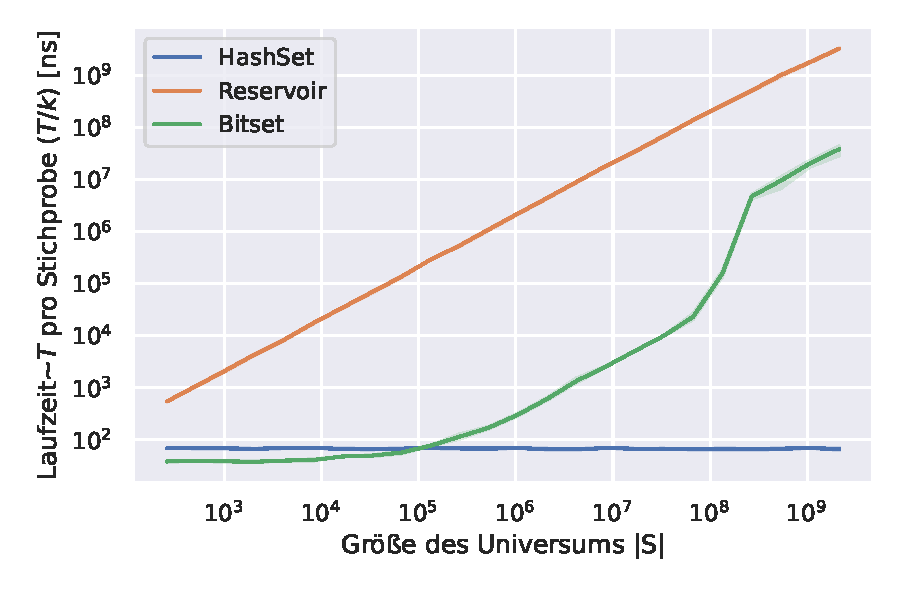
\includegraphics[width=0.32\textwidth]{data/gnm_scale0.pdf}\hfill
    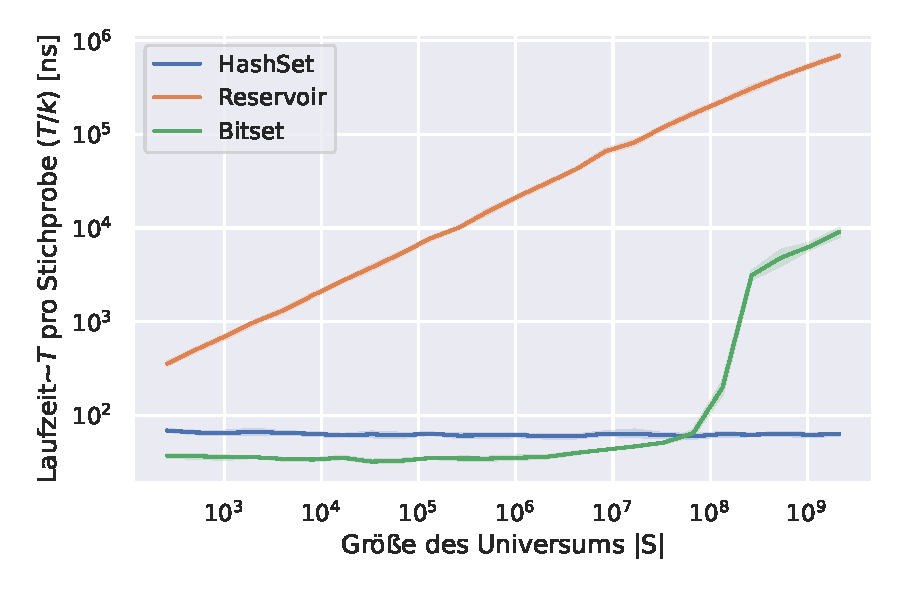
\includegraphics[width=0.32\textwidth]{data/gnm_scale1.pdf}\hfill
    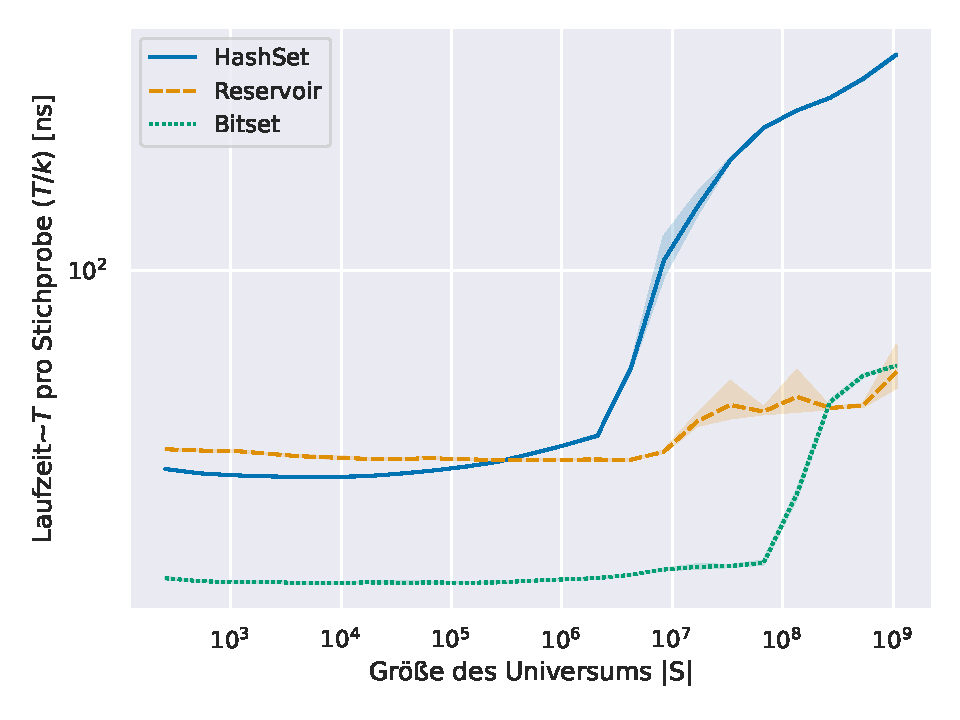
\includegraphics[width=0.32\textwidth]{data/gnm_scale2.pdf}

    \caption{
        Laufzeit~$T$ pro Sample~$k$ für das Ziehen von $k$ Elementen aus $S = \set{1, \ldots, N}$ als Funktion von $|S|$.\\
        \textbf{Links:} $k=10$, \textbf{Mitte: } $k = \sqrt{N}$, \textbf{Rechts: } $k = N / 4$.
    }
    \label{fig:benchmark_gnm_scale}
\end{widefigure}

In \cref{fig:benchmark_gnm_scale} stellen wir Laufzeitmessungen für folgendes Experiment dar.
Wir variieren die Größe unseres Universums $|S| = N$ von $2^8$ bis $2^{32}$ und betrachten drei Szenarien:
\begin{itemize}
    \item $k=10$: Trotz steigender Universumsgröße ziehen wir immer nur 10 Samples.
    \item $k=\sqrt{N}$: Die Stichprobengröße steigt langsam in der Universumsgröße (dieser Fall entspricht einem $\Gnm$ Graphen mit $m = \Theta(n)$).
    \item $k=N/4$: Jedes vierte Element des Universums wird ausgewählt.
\end{itemize}

\begin{exercise}
    Welche Effekte kannst du in \cref{fig:benchmark_gnm_scale} beobachten? Wie erklären sich diese?
\end{exercise}

Wir möchten uns aber nur auf einen zentralen Effekt in den Abbildungen konzentrieren, da dieser bei großen zufälligen Daten oft auftritt.\footnote{foreshadowing\ldots}
In \cref{fig:benchmark_gnm_scale} (rechts) beobachteten wir einen sprunghaften Anstieg der Zeit pro Element --- teils um fast einen Faktor 10.
Unsere Analysen sagen jedoch eine konstante Laufzeit pro gezogenem Element für $k = N/4$ voraus; einen sprunghaften Anstieg können sie nicht erklären.

Wir sind also im Algorithm-Engineering-Zyklus auf eine Diskrepanz zwischen Theorie und Praxis gestoßen!
Ist unsere Analyse falsch? Jaein.
In der Bestimmung der Laufzeit nutzen wir eine Unit-Cost Random-Access-Machine (d.h. wir gingen davon aus, dass jede Operation gleich viel Zeit benötigt).
Moderne Computer verfügen jedoch über ausgeklügelte Techniken, die gewisse Aspekte besonders beschleunigen.

Hierzu gehören die sog. Speicherhierarchien: Ein Prozessor kann nur auf Daten operieren, die sich auf dem physischen Chip befinden, genauer in den Registern.
Aus physikalischen und ökonomischen Gründen, gibt es aber nur sehr wenig \qq{Register-Speicher}.
Die meisten aktiven Daten werden daher im Arbeitsspeicher vorgehalten; dieser ist aber recht langsam.
Eine typische CPU kann in der Zeit, die es dauert ein Datum aus dem Arbeitsspeicher zu beziehen, etwa 100 bis 1000 Operationen ausführen.
Um dies aufzufangen, werden mehrere Caches eingefügt: die CPU \qq{rät} welche Daten in naher Zukunft benötigt werden und hält diese im schnelleren Cache vor.
Dies klappt aber mit Zufallsdaten oft nicht (sie sollen ja gerade \emph{nicht} vorhersehbar sein).

In \cref{fig:benchmark_gnm_scale} (rechts) sehen wir also genau den Punkt ab dem die Datenstrukturen nicht mehr in den Cache passen.
Für Hashset und Reservoir-Sampling nutzen diese Datenstrukturen etwa $64 k = 16 N$ Bits (das Hashset aufgrund des Load-Factors < 1 auch ein bisschen mehr).
Das Bitset benötigt $N$ Bits --- daher kommt hier der Performanceeinbruch auch später.

Um über diese qualitative Erklärung hinaus, das Verhalten analytisch zu erklären, benötigen wir also ein Maschinenmodell, das auch Speicherzugriffe berücksichtigt.
Dem widmen wir uns aber erst später.
Im Folgenden betrachten wir stattdessen eine Parallelisierung des Algorithmus --- dieselbe Strategie führt jedoch auch zu einem Generator, der zufällige Speicherzugriffe auf den Cache beschränken kann.
Wir brauchen zunächst ein Maschinenmodell für parallele Berechnungen.

\subsection{Fork-Join Parallelismus}
Das Fork-Join-Modell ist eine Erweiterung der Random-Access-Machine, welche die RAM um die zwei namesgebenenden Instruktionen erweitert.
Eine Berechnung startet als gewöhnliches sequentielles Programm, einem sog. Task.
Angenommen wir führen gerade $t_0$ aus, dann können wir die Berechnung in zwei \glqq Kindertasks\grqq{} $t_1$ und $t_2$ teilen \aside{fork} (\emph{forken}).
Beide Tasks werden unabhängig von einander ausgeführt, während $t_0$ ruht.
Sobald $t_1$ und $t_2$ fertig sind, kommt es zur Wiedervereinigung \aside{join} (\emph{join}):
$t_1$ und $t_2$ werden \glqq gelöscht \grqq, $t_0$ wieder geweckt und setzt seine Berechnung fort.
Betrachten wir das parallele Summieren $\sum_{i=1}^n x_n$ von Zahlen $X = (x_1, \ldots, x_n)$ als einfaches Beispiel:

\begin{algorithm}
    \SetKwProg{Fn}{Function}{}{end}
    \SetKwFunction{ParSum}{ParSum}
    \SetKwFunction{Fork}{Fork}
    \SetKwFunction{Join}{Join}
    \Fn{\ParSum{$X=(x_1, \ldots, x_n)$}}{
        \If{$n = 1$}{
            gebe $x_1$ zurück und beende Task\;
        }
        Berechne Mitte~$m \gets \lfloor n/2\rfloor$\;
        \Fork{$
                \underbrace{\ParSum{$X_L = (x_1, \ldots, x_m)$}}_{\text{Task $t_1$}}, \ \
                \underbrace{\ParSum{$X_R = (x_{m + 1}, \ldots, x_n)$}}_{\text{Task $t_2$}}
            $}\;
        $(s_1, s_2) \gets \Join{$t_1, t_2$}$\;
        gebe $s_1 + s_2$ zurück und beende Task
    }
    \caption{Parallele Summe im Fork-Join Modell}
    \label{algo:parallel_sum}
\end{algorithm}

In \cref{algo:parallel_sum} teilen wir die Eingabe rekursiv in zwei gleich große Teile (modulo Rundung) und berechnen die Teilsummen für beide rekursiv.
Sobald die Teilergebnisse vorliegen, summieren wir diese in $\Oh{1}$ Zeit und geben es als Gesamtergebnis zurück.
Dieses Schema funktioniert analog für alle assoziativen Operationen (z.B. Produkt, Min, Max).

In der Praxis findet man einige Software-Bibliotheken, die Fork-Join-Parallelismus zur Verfügung stellen;
für C++ etwa \texttt{Cilk} oder Intels \texttt{oneTBB}, für Rust \texttt{rayon}.
Diese praktischen Lösungen nutzen einen sog. Work-Stealing-Scheduler.

Grob \aside{Work Stealing} kann man annehmen, dass der Prozessor~$P_0$, der $t_0$ ausführte den Task $t_2$ als verfügbar bekannt gibt und dann selbst $t_1$ ausführt.
Wenn während der Ausführung von $t_1$ ein anderer Prozessor verfügbar ist, übernimmt dieser $t_2$.
In diesem Fall sind $t_1$ und $t_2$ also nebenläufig.
Wenn sich kein anderer Prozessor findet, wird $P_0$ den Task $t_2$ übernehmen, sobald $t_1$ beendet wurde.
Wir erhalten also ein dynamisches System, das (i) nicht wissen muss, wie viele Prozessoren es gibt, und (ii) auch relativ gut damit umgehen kann, dass $t_1$ und $t_2$ evtl. sehr unterschiedliche Laufzeiten haben.
Praktisch ist es kein Problem viel mehr Tasks zu erzeugen als es Prozessoren gibt.

Wir messen die Güte eines Fork-Join-Algorithmus mit zwei Eigenschaften:
\begin{enumerate}
    \item
          Die \aside{Arbeit / work} \emph{Arbeit} (engl. work) ist die Summe aller Instruktionen, die das Programm ausführt.
          Dies entspricht also der Laufzeit, wenn nur ein Prozessor zur Verfügung steht.
          Für \cref{algo:parallel_sum} ergibt sich die Arbeit als
          \begin{equation}
              W(n) = \begin{cases}
                  \Oh{1}                  & \text{falls } n = 1 \\
                  2 \cdot W(n/2) + \Oh{1} & \text{falls } n > 1
              \end{cases}
              = \Oh{n}.
          \end{equation}

          Der \aside{arbeits-optimal} Algorithmus leistet also asymptotisch nicht mehr Arbeit als die Laufzeit der besten sequentiellen Lösung; wir sagen er ist \emph{arbeits-optimal}.

    \item
          Der \aside{Span / Parallel Depth} Span (engl. span oder parallel depth) misst die Anzahl der Instruktionen auf einem kritischen Pfad (d.h. eine längste Folge abhängiger Schritte).
          Dies entspricht der Laufzeit, wenn wir unbeschränkt viele Prozessoren zur Verfügung haben.
          In \cref{algo:parallel_sum} müssen wir also analysieren, wie viele Instruktionen vor und nach dem Fork/Join Paar erforderlich sind und wie tief die Rekursion läuft:
          \begin{equation}
              S(n) = \underbrace{\Oh{1}}_\text{Arbeit vor/nach Fork/Join} + \underbrace{S(n/2)}_\text{Rekursion} = \Oh{\log n}.
          \end{equation}
\end{enumerate}

Wenn wir ausreichend Prozessoren zur Verfügung haben, können wir also $n$ Zahlen in Zeit $\Oh{\log n}$ summieren.
Zu ähnlichen Ergebnissen kommt man auch in anderen parallelen Maschinenmodellen (z.B. P-Rams).

\subsection{Rekursives Ziehen}
In \cref{algo:parallel_sum} haben wir bereits ein gutes Grundgerüst für parallele Algorithmen gesehen:
wenn wir es schaffen das Problem \emph{schnell} in unabhängige Hälften zu teilen und dann rekursiv zu bearbeiten, sind wir auf einem guten Weg.
Bezogen auf unser Problem, $k$~Stichproben aus $N$~Elementen zu ziehen, haben wir zwei Dimensionen:
\begin{enumerate}
    \item Teile $S$ deterministisch in $S_1$ und $S_2$: Wir können das Universum~$S$ mit $|S| = N$ in zwei Hälften $S_1$ und $S_2$ partitionieren mit $|S_1| = \lfloor N / 2 \rfloor$.
          Dann stellt sich die Frage: was ist die Anzahl~$k_1$ der Samples aus $S_1$, bzw. $k_2$ aus $S_2$. Klar ist nur $k_1 + k_2 = k$.

    \item Teile $k$ deterministisch in $k_1$ und $k_2$: Wir können die Stichproben teilen, d.h. $k_1 = \lfloor k/n \rfloor$ wählen; dann müssen wir jedoch eine unbekannte Partitionierung von $S$ finden.
\end{enumerate}

Auf den ersten Blick wirkt die zweite Variante zielführender.
Es ist vorteilhaft, wenn beide Teilprobleme etwa die gleiche Stichprobenanzahl haben, da die Arbeit in dieser Anzahl skalieren soll.
Tatsächlich liefert aber die erste Variante einfachere Algorithmen, die auch keine signifikanten Probleme mit unbalancierten Teilproblemen haben.

\begin{figure}[t]
    \begin{center}
        \begin{tikzpicture}
            \foreach \x in {-8, -4, -2, 3, 5, 7, 9} {
                    \node[inner sep=0, minimum size=1em, fill=black!20, anchor=west] at (\x em, 0) {};
                }

            \node[draw, minimum height=1em, minimum width=20em] at (0,0) {};
            \node[anchor=north] at (-9.5em, -0.5em) {1};
            \node[anchor=north] at ( 9.5em, -0.5em) {$N$};

            \foreach \x in {-9,...,9} {
                    \path[draw, black!50] (\x em, 0.5em) to ++(0, -1em);
                }

            \path[draw, thick, dashed] (0, 2em) to (0, -3.5em);

            \draw[decorate, decoration = {brace}] (-9.75em,3em) to node[above] {$k$} ++(19.5em,0);
            \draw[red,  decorate, decoration = {brace}] (-9.5em,1em) to node[above] {$k_1$} ++(9em,0);
            \draw[blue, decorate, decoration = {brace}] ( 0.5em,1em) to node[above] {$k_2$} ++(9em,0);

            \node[anchor=east] at (-12em, 1.8em) {zufällig:};

            \draw[decorate, decoration = {brace, mirror}] (-9.75em,-4em) to node[below] {$N$} ++(19.5em,0);
            \draw[red,  decorate, decoration = {brace, mirror}] (-9.5em,-2em) to node[below] {$N / 2$} ++(9em,0);
            \draw[blue, decorate, decoration = {brace, mirror}] ( 0.5em,-2em) to node[below] {$N / 2$} ++(9em,0);

            \node[anchor=east] at (-12em, -2.8em) {deterministisch:};

        \end{tikzpicture}
    \end{center}
    \caption{
        Ziehen von $k=7$ Stichproben aus $N=20$ Elementen ohne Zurücklegen; die grauen Elemente seien ausgewählt.
        Die linke Hälfte des Universums liefert $k_1$ Stichproben, die rechte $k_2$.
        Im gezeigten Beispiel gilt $k_1 = 3$ und $k_2 = 4$.
    }
    \label{fig:rekursive_k_aus_N}
\end{figure}


Wie in \cref{fig:rekursive_k_aus_N}, teilen wir also das Universum~$S$ in zwei gleich große Hälften $S_1$ und $S_2$.
Angenommen, wir täten dies nicht, wie viele Stichproben $k_1$ würde ein anderer Algorithmus aus $S_1$ ziehen?
Wir wissen es nicht genau, da $k_1$ eine Zufallsvariable ist --- sie ist Hypergeometrisch verteilt:
aus einer Gesamtpopulation von $N$ mit $k$~Treffern (d.h. die Elemente, die ein anderer Algorithmus gezogen hätte), ziehen wir $N_1$ Stichproben und erhalten $k_1$~Treffer.
In Erwartung sind es also $\expv{k_1} = k |S_1| / |S|$.

Analog zu den zufälligen Sprüngen in \cref{subsec:gnp_zufaellige_spruenge}, ziehen wir $k_1$ aus einer Hypergeometrisch Verteilung.
Dann setzen wir den Prozess bedingt auf $k_1$ fort:

\begin{algorithm}
    \SetKwProg{Fn}{Function}{}{end}
    \SetKwFunction{ParSelect}{ParSample}
    \SetKwFunction{Fork}{Fork}
    \SetKwFunction{Join}{Join}
    \Fn{\ParSelect{$S=(s_1, \ldots, s_N), k$}}{
        \If{$k = 1$}{
            $x \gets$ zufällig uniform aus $S$\;
            gebe $\set{x}$ zurück und beende Task\;
        }
        \BlankLine
        $N_L \gets \lfloor N / 2 \rfloor$\;
        $k_L \gets$ zufällig hypergeometrisch: ziehe $N_L$ Element aus $N$ mit $k$ Treffern\;
        \BlankLine
        \Fork{$
                \underbrace{\ParSelect{$S_L = (s_1, \ldots, s_{N_L}), k_L$}}_{\text{Task $t_1$}}, \ \
                \underbrace{\ParSelect{$S_R = (s_{N_L + 1}, \ldots, s_N), k - k_L$}}_{\text{Task $t_2$}}
            $}\;
        $(R_1, R_2) \gets \Join{$t_1, t_2$}$\;
        gebe $R_1 \cup R_2$ zurück und beende Task
    }
    \caption{Paralleles Ziehen von $k$ Stichproben aus $S$ ohne Zurücklegen}
    \label{algo:parallel_k_aus_N}
\end{algorithm}

\goodbreak

\noindent
Um die Performance von \cref{algo:parallel_k_aus_N} zu analysieren, treffen wir zwei Annahmen:
\begin{enumerate}
    \item Wir können $S$ in $\Oh{1}$ Zeit in zwei (fast) gleich große Hälften teilen.
          Das ist in vielen Fällen möglich:
          \begin{itemize}
              \item Für $\Gnm$ Graphen gehen wir davon aus, dass $S$ nur implizit existiert und das Intervall $[1, n^2]$ repräsentiert.
                    Dies können wir durch Verschieben der Intervallgrenzen trivial in $[1, n^2 / 2]$ und $[n^2/2 + 1, n^2]$ teilen.
              \item Wenn $S$ ein Array ist, können in die Rekursion Pointer auf den Anfang und das Ende des Teilproblems gegeben.
          \end{itemize}

    \item Die Operationen $R_1 \cup R_2$ läuft in konstanter Zeit.
          Das ist realistisch: da die Elemente in der Menge $S$ paarweise verschieden sind, wissen wir, dass $|R_1 \cup R_2| = |R_1| + |R_2| = k$.
          Es ist also kein Test auf Duplikate o.Ä. notwendig und es reicht aus $R_1$ und $R_2$ zu konkatenieren.
          Das ist mit verketten Listen (inkl. Endpointer) in $\Oh{1}$ Zeit möglich.
\end{enumerate}

\begin{exercise}
    Angenommen wir möchten $R$ als Array bekommen.
    Zeige, dass es möglich ist $R$ eingangs mit einer Kapazität von $k$ zu initialisieren, und dann in der Rekursion direkt in $R$ zu schreiben.
    Die Samples sollen dann in derselben relativen Reihenfolge wie in $S$ erscheinen.
\end{exercise}

\begin{lemma}
    \Cref{algo:parallel_k_aus_N} hat mit hoher Wahrscheinlichkeit einen Span von $\Oh{\log k}$ und benötigt in Erwartung $\Oh{k}$ Arbeit.
\end{lemma}

\begin{widefigure}
    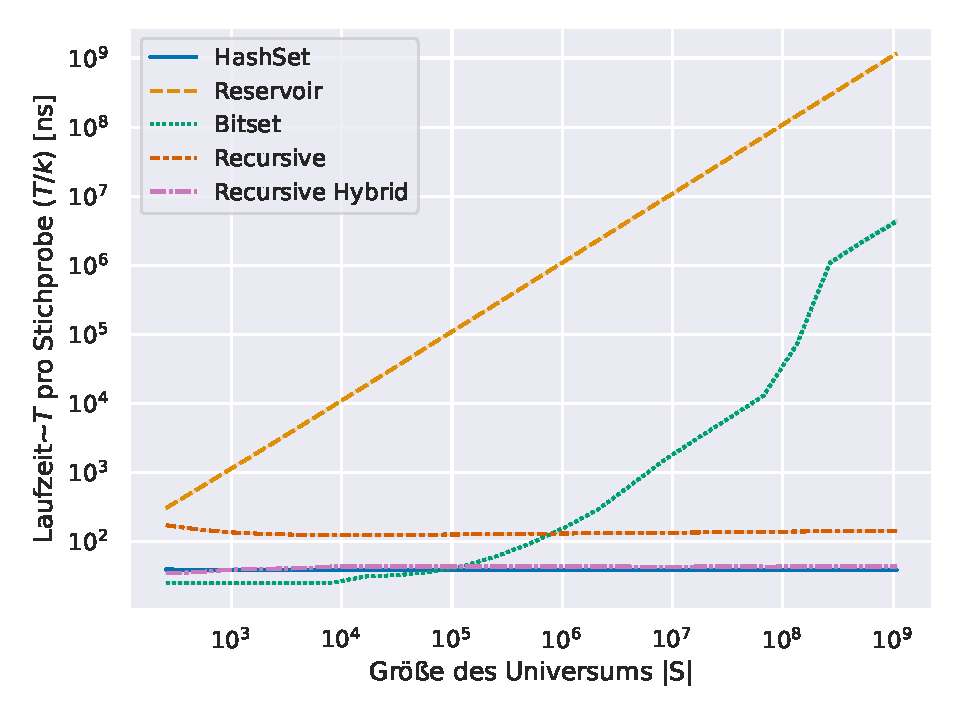
\includegraphics[width=0.32\textwidth]{data/gnm_recursive_scale0.pdf}\hfill
    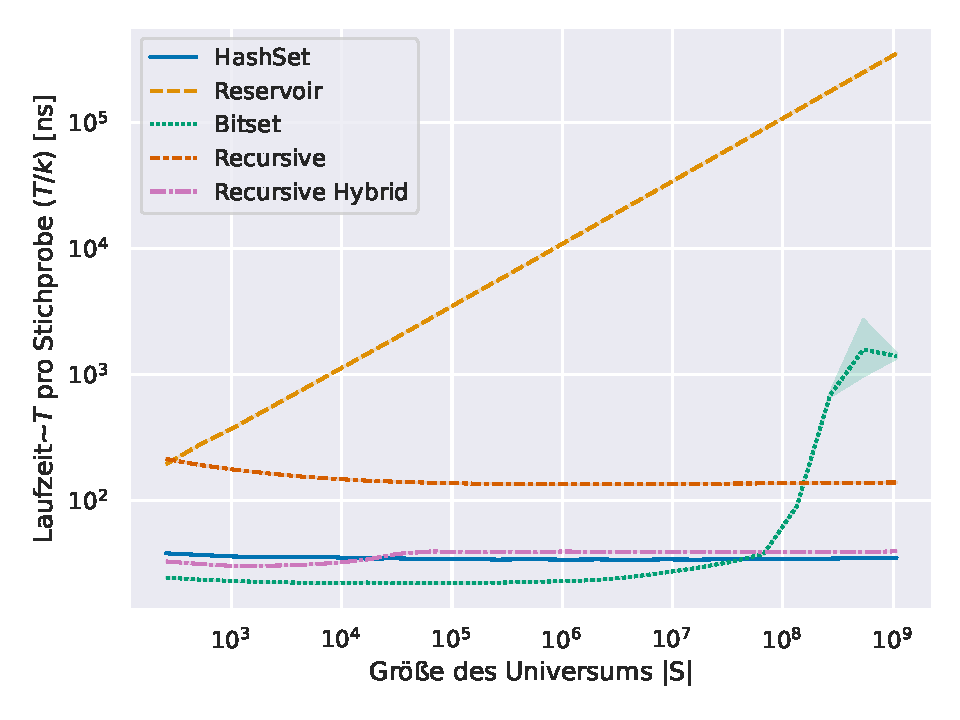
\includegraphics[width=0.32\textwidth]{data/gnm_recursive_scale1.pdf}\hfill
    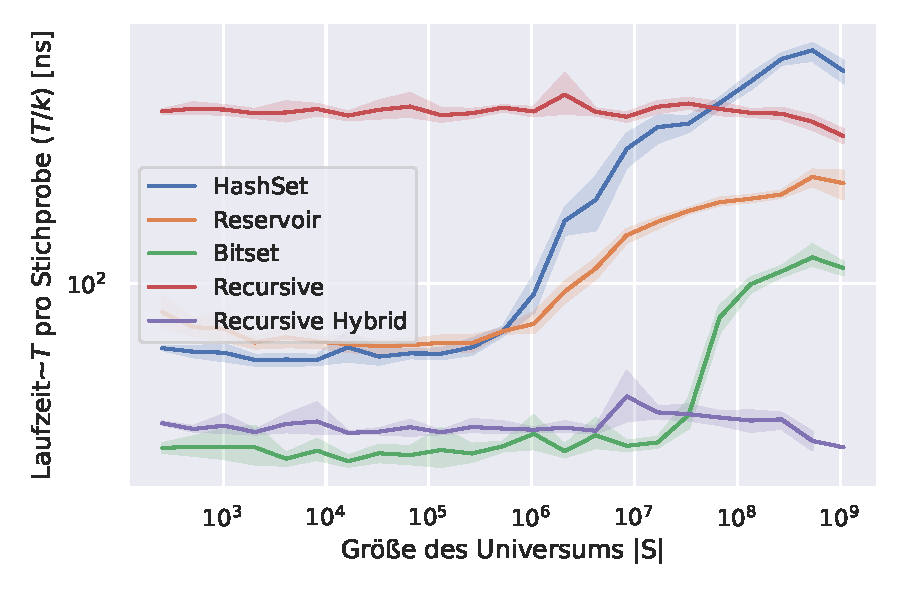
\includegraphics[width=0.32\textwidth]{data/gnm_recursive_scale2.pdf}

    \caption{
        Laufzeit~$T$ pro Sample~$k$ für das Ziehen von $k$ Elementen aus $S = \set{1, \ldots, N}$ als Funktion von $|S|$.\\
        \textbf{Links:} $k=10$, \textbf{Mitte: } $k = \sqrt{N}$, \textbf{Rechts: } $k = N / 4$.
    }
    \label{fig:benchmark_gnm_recursive_scale}
\end{widefigure}

Wir überspringen den Beweis; dieser lässt sich aber analog zu \cite{DBLP:journals/toms/Hubschle-Schneider22} führen.
Die Hauptideen sind: ein Span von $\Oh{\log N}$ folgt trivial wie in unserem Beispiel zum parallelen Summieren, dadurch dass wir in jedem Schritt die Größe von $|S|$ halbieren.
Um den Span jedoch auf $\Oh{\log k}$ zu reduzieren, müssen wir zeigen, dass sich auch die Stichprobengröße ungefähr gleich auf beide Teilprobleme verteilt.
Dies folgt aus der relativ kleinen Varianz der Hypergeometrischen Verteilung für hinreichend großes $k$.
Nur für sehr kleines $k$ laufen wir Gefahr, dass eines der beiden Teilprobleme alle Samples enthält;
das ist aber zum einen unkritisch (weil $|S|$ trotzdem halbiert wird und so die Dichte $k/N$ steigt) und zum anderen, wie wir gleich sehen werden, für praktische Implementierungen unerheblich.

Wie in \cref{fig:benchmark_gnm_recursive_scale} gezeigt, zeigt eine (sequentielle) Implementierung von \cref{algo:parallel_k_aus_N} ein gutes Skalierungsverhalten.
Die Laufzeit hängt nur von $\Oh{k}$ ab und steigt nicht für großes $N$ --- sie ist jedoch allgemein recht hoch (das Ziehen einer Hypergeometrischen Zufallsvariable ist recht langsam).
Dies \aside{Rekursionsstopper} ist ein sehr gängiges Problem in komplexen Algorithmen mit einer einfachen Lösung.
Wir verwenden den aufwendigeren Algorithmus nur so lange, wie es von Vorteil ist.
Wenn die Teilprobleme hinreichend klein sind und wir alle Prozessoren auslasten, schalten wir als \qq{Rekursionsstopper} auf spezielle Basisalgorithmen um, die sich besonders gut für kleine Teilprobleme eignen.
Der Hybridalgorithmus in \cref{fig:benchmark_gnm_recursive_scale} nutzt, für große $N$ den rekursiven Ansatz.
Für kleine Teilprobleme mit $N < 10\,000$ kommt  ---je nach Dichte $k/N$--- entweder BitSet oder HashSet zum Einsatz.

\section{Phasenübergänge in \Gnp und \Gnm}
Die ersten analytischen Ergebnisse von Zufallsgraphen betrafen das Verhalten von kombinatorischen Eigenschaften für verschiedene Dichten (d.h. $m/n$ bei $\Gnm$, bzw $p$ bei $\Gnp$) im Grenzwert für $n \to \infty$.
In \aside{Wir nutzen ungerichtete Graphen und setzen $N = \binom n 2$} diesem Kapitel werden wir uns auf ungerichtete Graphen konzentrieren.

Betrachten wir zunächst \Gnm Graphen.
Für diese zeigten Erd\H{o}s und R\'enyi bereits 1960 einige Schwellwerte an denen sog. Phasenübergänge stattfinden.
Für \emph{sehr} dünne Graphen mit $m(n) = o(\sqrt n)$, bewiesen sie etwa, dass diese wahrscheinlich nur isolierte Knoten und Kanten beinhalten.
Wir wollen uns an dieser Aussage ansehen, wie man die Wahrscheinlichkeit eines solchen Ereignisses abschätzen kann.

\begin{lemma}
    Sehr dünne $\Gnm$ Graphen mit $m = o(\sqrt n)$ haben für $n \to \infty$ wahrscheinlich keine Knoten mit mehr als einer Kante.
\end{lemma}

\begin{proof}
    Sei $p(n,m)$ die Wahrscheinlichkeit, dass keine zwei Kanten einen gemeinsamen Endpunkt haben.
    Wir vergleichen nun die Anzahl der möglichen Graphen mit der Anzahl der günstigen Graphen (d.h. ohne zwei Pfade).
    Zunächst beobachten wir, dass es $|\mathbb G(n,m)| = \binom N m = \binom{\binom n 2}{m}$ verschiedene $\Gnm$ Graphen gibt.
    Wie viele von diesen haben keine Knoten mit mindestens Kanten?

    Stellen wir uns dazu vor, dass wir die Kanten $E = \set{\set{u_1, v_1}, \ldots, \set{u_m, v_m}}$ erstellen, indem wir $2m$ Knoten $u_1, v_1, u_2, v_2, \ldots, u_m, v_m$ ziehen.
    Da keine zwei Kanten einen gemeinsamen Endpunkt haben sollen und Schleifen verboten sind, müssen wir also $2m$ \underline{verschiedene} Knoten ziehen!
    Es ist aber egal, in welcher Reihenfolge wir die $m$~Kanten ziehen und ob ein Endpunkt als $u_i$ oder $v_i$ gezogen wird.
    Die Anzahl ergibt sich also als
    \begin{align}
        \frac{
            \overbrace{\binom{n}{2m}}^\text{$2m$ verschiedene Knoten aus $n$}
            \overbrace{(2m)!}^\text{Mögliche Permutation von $2m$ Elementen}
        }{
            \underbrace{m!}_\text{Reihenfolge der Kanten egal\ \ \ }
            \underbrace{2^m}_\text{Reihenfolge in einer Kante egal}
        }.
    \end{align}

    \noindent
    Die wir jeden möglichen Graphen mit derselben Wahrscheinlichkeit ziehen, gilt
    \begin{align}
        \bar p(n, m) = \frac{\binom{n}{2m} (2m)!}{m! 2^m \binom{\binom n 2}{m}} \label{eq:wkeit_keine_zwei_kanten}
    \end{align}

    \noindent
    Wir werden im Folgenden eine \emph{untere} Schranke für $\bar p(n,m)$ zeigen.
    Dazu nutzen wir folgende Abschätzung von $\binom n k$

    \begin{align}
        \binom n k \approx \frac{n^k \exp\left(-\frac{k^2}{2n} - \frac{k^3}{6n^2}\right)}{k!}
        \quad\quad \text{für } k = o(n^{3/4}).
    \end{align}

    Der Einfachhalt halber verzichten wir auf die Analyse des Fehlers dieser Abschätzung.
    Es folgt
    \begin{align}
        p(n, m)
         & \ge \frac{\binom{n}{2m} (2m!)}{m! 2^m \binom{n^2/2}{m}}                                                                                   \\
         & = \frac{\textcolor{blue}{\binom{n}{2m}}(2m!)}{\textcolor{red}{\binom{n^2/2}{m}} m! 2^m}                                                   \\
         & \approx \frac{
        \textcolor{blue}{n^{2m} \exp\left(-2\frac{m^2}{n} - \frac{8m^3}{6n^2}\right)}\textcolor{red}{m!}(2m!)
        }{
        \textcolor{blue}{(2m)!}\textcolor{red}{\underbrace{(n^2/2)^m}_{=n^{2m} / 2^m} \exp\left(-2\frac{m^2}{n^4} - \frac{8m^3}{6n^6}\right)} m!2^m} \\
         & = \exp\left(-2\frac{m^2}{n} (1 - \frac{1}{n^3}) - \frac{8m^3}{6n^2} (1 - \frac{1}{n^4}) \right)                                           \\
         & \ge \exp\left(-2\frac{m^2}{n} - \frac{8m^3}{6n^2} \right)                                                                                 \\
         & \ge \exp\left(-4\frac{m^2}{n} \right) \quad \text{für hinreichend großes $n$}
    \end{align}

    Damit gilt also $\lim_{n \to \infty} p(n, m(n)) = 1$ falls $m(n) = o(n)$.
\end{proof}

Beobachte, dass \cref{eq:wkeit_keine_zwei_kanten} eine exakte Wahrscheinlichkeit ist, die wir erst im Nachgang von unten abschätzen.
Durch eine geeignete obere Schranke lässt sich zeigen, dass für $m \ge c \sqrt n$ für ein konstantes $c > 0$ (d.h. nicht von $n$ abhängig) die Wahrscheinlichkeit mindestens eines Knotens mit mindestens zwei Nachbarn gegen $1$ geht.
Wir sagen daher, dass \Gnm Graphen einen Phasenübergang mit Schwellwertfunktion $m(n) = \sqrt n$ haben.


\bigskip

Wir wechseln nun zu \Gnp Graphen.
Hier werden wir einen Beweis sehen, der die Unabhängigkeit aller Kanten ausnutzt.
Zuerst schauen wir uns aber einige wohlbekannte Phasenübergänge an.
Sei $\epsilon >0$ hinreichend klein.
Dann gilt:
\begin{itemize}
    \item Falls $np < 1 - \epsilon$ haben mit hoher Wahrscheinlichkeit alle Zusammenhangskomponenten Größe $\Oh{\log n}$.
    \item Falls $np = 1$ hat die größte Zusammenhangskomponente mit hoher Wahrscheinlichkeit Größe $\Theta(n^{2/3})$.
    \item Falls $np > 1$ gibt es mit hoher Wahrscheinlichkeit eine einzelne Zusammenhangskomponente mit Größe $\Theta(n)$.
          Keine andere Komponente hat mehr als $\Oh{\log n}$ Knoten.

    \item Falls $np < (1-\epsilon)\log n$ gibt es mit hoher Wahrscheinlichkeit einzelne Knoten ohne inzidente Kanten.
    \item Falls $np > (1+\epsilon)\log n$ ist der Graph mit hoher Wahrscheinlichkeit zusammenhängend.
\end{itemize}

\begin{exercise}
    Zeige ein möglichst großes $p(n)$ für das $\Gnp$ Graphen mit hoher Wahrscheinlichkeit keine Kanten haben.
\end{exercise}

Wir möchten nun das Verhalten um $np = 1$ besser verstehen und folgen einem algorithmischen Beweis von \cite{DBLP:journals/rsa/KrivelevichS13}.
Die Idee ist relativ einfach:
wir führen eine Tiefensuche auf einem $\Gnp$ Graphen aus, wobei die Nachbarschaft durch Ziehen von Einträgen in der Adjazenzmatrix erkundet wird.
Dann zeigen wir, dass für $np < 1$ so wenig Einsen vorhanden sind, dass es sehr unwahrscheinlich ist eine große Zusammenhangskomponente zu beobachten.
Für $np > 1$, hingegen, sehen wir ausreichend viele Einsen.

\subsection{Tiefensuche auf $\Gnp$}
Im Folgenden definieren wir eine klassische Tiefensuche (DFS) auf eine Weise, die für den folgenden Beweis hilfreich ist.
Implementieren sollte man sie so besser nicht...
Während einer DFS können wir die Knotenmenge~$V$ in drei Teilmengen $B$, $S$, $U$ partitionieren:
\begin{itemize}
    \item \underline Bearbeitete Knoten~$B$ sind Knoten, die besucht wurden und keine Kinder in $U$ mehr haben.
    \item Knoten in~$S$ werden gerade erkundet und liegen daher auf dem \underline Stack.
    \item \underline Unbekannte Knoten wurden noch nicht gefunden.
\end{itemize}

Bevor die DFS startet, gilt also $B = S = \emptyset$ und $U = V$.
Die Suche terminiert sobald $B = V$ und $S = U = \emptyset$.
Solange dies noch nicht der Fall ist, wird einer der folgenden Schritte ausführt:

\begin{enumerate}
    \item Falls $S \ne \emptyset$ sei $v$ der Knoten, der als letztes eingefügt wurde ($S$ ist ein Stack)
          \begin{enumerate}
              \item Falls $v$ einen Nachbarn $w \in U$ hat: entferne $w$ aus $U$ und füge $w$ in $S$ ein
              \item Falls nicht, ist $v$ vollständig bearbeitet: entferne $v$ aus $S$ und füge $v$ in $B$ ein
          \end{enumerate}
    \item Falls $S = \emptyset$ entnehme den ersten Knoten $v \in U$ und füge ihn in $S$ ein
\end{enumerate}

Um Uneindeutigkeiten zu vermeiden, fixieren wir die Knotenordnung.
Hierzu nehmen wir oBdA an, dass $V = \set{1, \ldots, n}$ natürliche Zahlen sind.
Die Mengen $V$ und $U$ seien aufsteigend geordnet, insbesondere werden immer die kleinsten passenden Elemente entnommen (in Schritten 1a und 2).
Weiter, sei $S$ ein Stack, d.h. das Element, das als letztes eingefügt wurde, wird als erstes entfernt.

Das Besondere an unser DFS ist, dass wir keine Kantenliste als Eingabe bekommen, sondern uns verstellen, einen Strom von unabhängig zufälligen Bits $X_1, \ldots, X_N$ zu erhalten, wobei $\prob{X_i = 1} = p$.
Wenn wir nun in Schritt 1a einen Nachbar von $v$ suchen, iterieren wir gleichzeitig über $U$ und $X$.
Dann geben wir das erste $w$ zurück, dessen Bit gesetzt war (falls es existiert).
Wenn wir das nächste Mal mit Knoten $v$ zu Schritt 1a kommen, suchen wir nur nach $w' \in U$ mit $w' > w$ --- wir machen als an der Stelle weiter, an der wir einen Nachbarn gefunden haben.

\begin{exercise}
    Zeige, dass jeder Eintrag der Adjazenzmatrix höchstens einmal betrachtet wird und wir mittels der $X_i$ somit ein DFS auf \Gnp simulieren.
    Die zweite Beobachtung (s.u.) folgt hieraus.
\end{exercise}

\noindent
Wir werden später folgende Beobachtung ausnutzen:
\begin{itemize}
    \item In jeder Iteration wird ein Knoten entweder von $U$ nach $S$ (Schritt 1a oder 2) oder von $S$ nach $B$ (Schritt 1b).
          Es gibt also stetigen Fortschritt.
    \item Zu jedem Zeitpunkt gilt, dass der Graph keine Kanten zwischen $U$ und $B$ hat; insb. ändern noch nicht entdeckte Kanten hieran nichts mehr.
    \item Alle Knoten in $S$ gehören zur selben Zusammenhangskomponente.
\end{itemize}

\subsection{Zusammenhangskomponenten für $np = (1-\epsilon)$ sind klein}
Wenn wir nun DFS ausführen, werden wir unsere Strukturaussagen zu \Gnp auf Eigenschaften Stroms von Zufallsbits reduzieren.
Die Hauptarbeit dieser Analyse leisten wir in \cref{lemma:dfs_kaum_einsen_in_X}.

Der \aside{union bound} Beweis des Lemmas nutzt eine übliche Struktur.
Wir möchten zeigen, dass etwas nicht passiert, obwohl es viele Möglichkeiten $X_1, \ldots, X_n$ hierfür gibt.
Man schätzt also zunächst die Einzelwahrscheinlichkeiten~$\prob{X_i}$ ab (vereinfachend nimmt man oft an, dass die $X_i$ unabhängig sind).
Hier sollten sich extrem kleine Erfolgswahrscheinlichkeiten $\prob{X_i} < 1/n$.
Dann schätzt man die Wahrscheinlichkeit, dass mindestens eins eintritt, einfach als Summe der Einzelwahrscheinlichkeiten nach oben ab.
Booles \aside{Booles Ungleichung} Ungleichung besagt:
\begin{align}
    \prob{\bigcup_{i=1}^n X_i} = \prob{\text{mindestens ein $X_i$ tritt ein}} \le \sum_{i=1}^n \prob{X_i}
\end{align}

\noindent
Nun können wir eine wichtige Eigenschaft unserer Zufallsbits zeigen.
Wir befinden uns zunächst im subkritischen Bereich, sprich unsere Analyse betrachtet Graphen mit $np < (1 - \epsilon)$.

\begin{lemma}[basiert auf \cite{DBLP:journals/rsa/KrivelevichS13}]\label{lemma:dfs_kaum_einsen_in_X}
    Sei $\epsilon > 0$ \aside{kleines $\epsilon > 0$ \\ $N = \binom n 2$ \\ $p = (1 - \epsilon) / n$ \\ $k = (10 / \epsilon^2) \ln n$} eine hinreichend kleine Konstante und seien $X = (X_1, \ldots, X_N)$ unabhängige Zufallsvariablen, die Bernoulli mit Parameter~$p$ verteilt sind.
    %\begin{enumerate}
    %\item
    Sei $p = (1 - \epsilon) / n$ und $k = (10 / \epsilon^2) \ln n$.
    Dann gibt es mit hoher Wahrscheinlichkeit keine zusammenhängende Teilfolge (Intervall) mit Länge $nk$ (d.h. $X_i, \ldots, X_{i+nk}$) in dem mindestens $k$ Zufallsvariablen den Wert 1 haben.

    %\item Sei $p = (1 + \epsilon) /n$ und $N_0 = \epsilon n^2/2$.
    %      Dann gilt mit hoher Wahrscheinlichkeit $|\sum_{i=1}^{N_0} X_i - \epsilon(1+\epsilon)/2| \le n^{2/3}$.
    %      \qedhere
    %\end{enumerate}
\end{lemma}

\begin{proof}
    %Beginnen wir mit der ersten Aussage.
    Wir definieren $Y_i = \sum_{j=1}^{nk} X_{i+j-1}$ als die Anzahl an Einsen im Intervall, das mit $X_i$ beginnt.
    Aus Symmetrie können wir uns zunächst auf ein Intervall $Y_1$ beschränken.
    Mittels additiver Chernoff Ungleichung kann man zeigen
    \begin{align}
        \prob{Y_1 \ge k} < \exp\left(-\frac{\epsilon^2(1-\epsilon)}{3} \cdot \frac{10}{\epsilon^2} \ln n \right)
        = \exp\left(- \underbrace{(1-\epsilon)}_{\to 1} \frac{10}{3} \ln n \right)
    \end{align}

    Da die Behauptung nicht nur über ein Intervall~$Y_1$ spricht, sondern für über alle $Y_1, \ldots, Y_{N-nk}$, benötigen wir noch einen \emph{union bound}.
    Hierfür betrachten wir die Einzelereignisse $Y_i \ge k$ für alle $i$:

    \begin{align}
        \prob{\exists i:\ Y_i \ge k} & \le \sum_{i=1}^{N-k} \prob{Y_i \ge k}                                                                                        \\                                                                      \\
                                     & \le N \cdot \prob{Y_1 \ge k}                                                                                                 \\
                                     & \le \frac{n^2}{2} \ \cdot\ \underbrace{\exp\left(- \underbrace{(1-\epsilon)}_{\to 1} \frac{10}{3} \ln n \right)}_{=o(1/n^3)}
                                     & \le \frac{1}{2n}
    \end{align}

    Da die Gegenwahrscheinlichkeit durch $1/2n$ nach oben beschränkt ist, gilt die Aussage mit hoher Wahrscheinlichkeit.
\end{proof}

Wir wissen also, dass für $p < (1 - \epsilon) / n$, wir in $nk$ Zufallsbits ziemlich sicher keine $k$ Einsen finden.
Die Intuition für \Gnp ist also, dass wir in $k$ Zeilen der Adjazenzmatrix keine $k$ Nachbarn finden.
Diese $k$ Zeilen können also nicht zusammenhängend sein!
Wir formalisieren dieses Bauchgefühl in folgendem Theorem:

\begin{theorem}[basiert auf \cite{DBLP:journals/rsa/KrivelevichS13}]
    Sei \aside{$\Gnp$ mit $np = (1-\epsilon)$ hat nur Zusammenhangskomponenten mit $\Oh{\log n}$ Knoten.} $\epsilon > 0$ hinreichend klein.
    Ferner sei $G \sim \Gnp$ ein zufälliger Graph mit $np = (1 - \epsilon)$.
    Dann haben alle Zusammenhangskomponenten mit hoher Wahrsceinlichkeit eine Größe von höchstens $10 \epsilon^{-2} \ln n$.
\end{theorem}

\begin{proof}
    Beweis durch Widerspruch.
    Nehmen wir an, es gibt eine Zusammenhangskomponente~$K$ mit mehr als $k = 10 \epsilon^{-2} \ln n$ Knoten.
    Betrachten wir die Phasen in der DFS während $K$ exploriert wird.

    Konkret betrachten wir den Moment, zu dem der $k+1$ Knoten entdeckt wird (dieser wird also gleich von $U$ nach $S$ bewegt).
    Seien $\Delta K = K \cap B$ die Knoten der Zusammenhangskomponente~$K$ die bereits fertig bearbeitet wurden.
    Dann gilt $|\Delta K \cup S| = |\Delta K| + |S| = k$; sonst hätten wir nicht eben den $k+1$ Knoten entdecken können.

    Den ersten dieser $k$ Knoten bekamen wir \qq{kostenlos}, da er in Schritt 2 von $U$ nach $S$ bewegt wurde, um die Suche in der neuen Zusammenhangskomponente zu starten.
    Jeder weitere Knoten musste über eine Kanten zu einem Knoten in $\Delta K \cup S$ entdeckt wurden sein.
    Da Kanten zu einer Eins in unseren Zufallsbits korrespondiert, müssen wir als beim Entdecken des $k+1$ Knoten genau $k$ Einsen gesehen haben.

    Von jedem Knoten in $\Delta K \cup S$ suchten wir nach höchstens $n$ Nachbarn (grobe Überabschätzung!).
    In anderen wurden, wir haben höchstens $k n$ Bits gelesen und dabei $k$ Einsen gefunden.
    Das passiert gemäß \cref{lemma:dfs_kaum_einsen_in_X} mit hoher Wahrscheinlichkeit nicht.
\end{proof}

Durch geeignete Abschätzung, dass es für $np = (1 + \epsilon)$ \qq{viele} Einsen gibt, lassen sich folgende Resultate zeigen.
Mit hoher Wahrscheinlichkeit enthält $G \sim \Gnp$ \ldots
\begin{itemize}
    \item \ldots einen Pfad mit mindestens $\epsilon^2 n / 5$ Knoten.
    \item \ldots einen Kreis mit $\Theta(\epsilon^2) n$ Knoten.
    \item \ldots eine Zusammenhangskomponente mit mindestens $\epsilon n / 2$ Knoten.
\end{itemize}

Beobachte, dass die giant component deutlich größer ist als die Pfadlänge.
Dies ist inhaltlich richtig (und erwartet --- warum??), bedarf aber auch eine deutlich genaueren Abschätzung unserer Zufallsbits.

Weiter ist die $\epsilon^2$ Abhängigkeit der ersten beide Aussagen optimal.
Tatsächlich ist das Resultat zur Pfadlänge der Grund, weshalb wir uns eine Tiefensuche statt einer Breitensuche angesehen haben.
Wenn wir in der Tiefensuche jemals eine Stackgröße von $|S| = k$ erreichen, wissen wir, dass der untersuchte Graph einen Pfad mit mindestens $k$ Knoten enthält;
das gilt nicht für die Breitensuche!
Der Beweis zeigt also, dass wir ausreichend viele Einsen sehen um ein hinreichend großen Stack zu sehen.

\subsection{Existenz von großen Kreisen}
Zuletzt wollen wir uns noch eine Beweistechnik ansehen, bei der wir zwei geeignet parametrisiert $\Gnp$ durch Vereinigung ihrer Kantenmengen \qq{aufaddieren}.
Mit dieser Technik lässt sich aus der (mit hoher Wahrscheinlichkeit) Existenz eines Pfads mit $\alpha n$ Knoten $\alpha > 0$, die (mit hoher Wahrscheinlichkeit) Existenz eines Kreises mit $\Theta(\alpha n)$ Knoten folgern.
Hierzu ziehen wir einen weiteren $\mathcal G(n, p')$ Graphen mit ausreichend großen $p' = o(1/n)$.
Diese neuen Kanten fügen wir zu unserem ursprünglichen Graphen $G$ hinzu und erhalten $G' \sim \mathcal G(n, p'')$ mit $p'' \lessapprox p + p'$.
Da $p' = o(1/n)$ ist $p + p' = (1+\epsilon)/n + o(1/n)$ für $n \to \infty$ weiterhin durch $p$ dominiert.

Zur einfacheren Illustration nehmen wir $p' = n^{-3/2} = o(1/n)$ an.
Weiter betrachten wir die ersten und letzten $\ell = 2 n^x$ Knoten des Pfades mit hinreichend großem $x < 1$.
Es bleibt ein Mittelteil von $M$ Knoten \qq{übrig}:
\begin{align}
    M = \alpha n - 2\ell =\alpha n - 4 n^x =  n(\alpha - \underbrace{4n^{x - 1}}_{=o(1)\text{, da } x < 1})
\end{align}

Im Grenzwert von $n\to\infty$, sind also der Präfix und Suffix des Pfades relativ zum Mittelteil asymptotisch verschwindet klein.

Es gibt aber $\binom{\ell}{2} \ge n^{2x}$ mögliche Kanten zwischen dem Präfix und dem Suffix.
Aus $G'$ bekommen wir also erwartet mehr als $n^{2x} p'$ Kanten --- eine reicht um einen einen Kreis, der länger als $M$ ist, zu schließen.
In unserem Beispiel mit $p = n^{-3/2}$ gilt:
\begin{align}
    n^{2x} p' = n^{2x - 3/2}
\end{align}

Wenn wir also $x = 3/4$ wählen, erwarten wir mindestens eine Kante, die dann den versprochenen Kreis schließt.
Für $x > 3/4$ existiert eine solche Kante mit hoher Wahrscheinlichkeit.

\section{Gradverteilung}


\chapter{Knotengrade}
% !TeX root = skript.tex
\emph{Die nichtalgorithmischen Aspekte dieses Kapitels orientiert sich stark an \cite{barabasi2014network}.}
\bigskip

\noindent
Eine elementare Aufgabe in Network Science ist es, die Wichtigkeit von Knoten zu bewerten -- man spricht auch \aside{Zentralität: Wichtigkeit eines Knotens} von der \emph{Zentralität} der Knoten.
Die Anzahl der Nachbarn (Grad, engl. degree) ist eine sehr einfache Metrik mit direkter Intuition:
Wenn ein Knoten überdurchschnittlich viele Nachbarn hat, dann steht die Vermutung im Raum, dass diesem Knoten auch eine überdurchschnittlich wichtige Bedeutung im Netzwerk zukommt.
Daher wollen wir die Verteilung von Graden in Graphen in diesem Kapitel genauer betrachten.

Zur Wiederholung:
In einem ungerichteten Graphen~$G=(V,E)$ beschreibt
\begin{equation}
    \deg(u) = \card{\twoset{e}{e \in E\text{, \sd\ } u \in e}}
\end{equation}
die Anzahl der Nachbarn von Knoten~$u$.
Die \aside{Grad\underline{sequenz}} Gradsequenz~$\degseq_G$ (falls $G$ klar ist, auch nur $\degseq$) von $G=(V,E)$ mit $V=\set{v_1, \ldots, v_n}$ ist dann einfach die Auflistung aller Grade im Graphen
\begin{equation}
    \degseq_G = (\deg(v_1), \deg(v_2), \ldots, \deg(v_n)).
\end{equation}
Beobachte, dass für jede $\degseq_G$ von $G=(V,E)$ gilt:
\begin{equation}
    \sum_{v \in V} \deg(v) = 2 \card{E}
\end{equation}


\section{Knotengrade in $\Gnp$}
\begin{figure}
    \begin{center}
        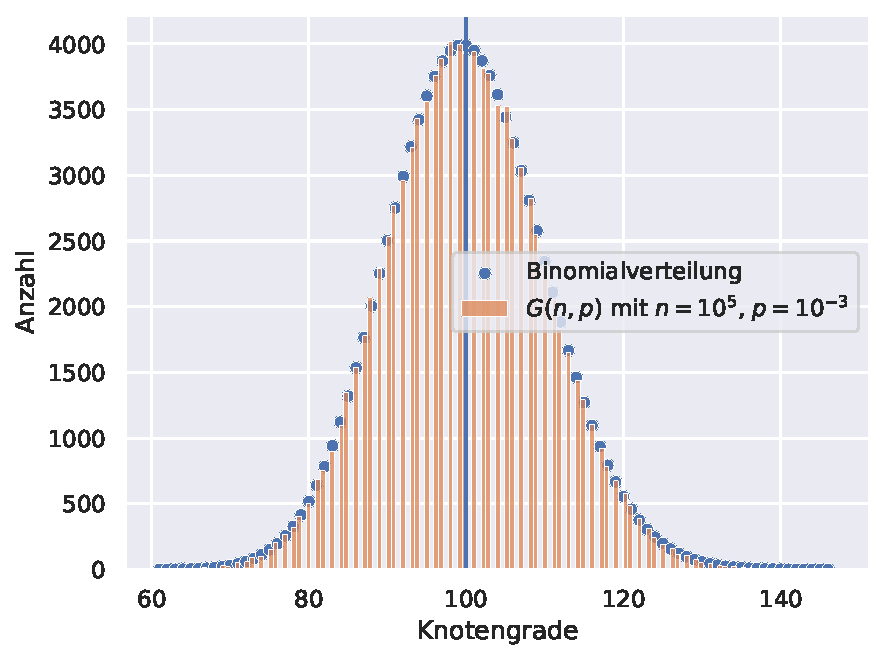
\includegraphics[width=0.6\textwidth]{data/gnp_degrees.pdf}
    \end{center}
    \caption{
        Histogramm der Gradsequenz~$\degseq_G$ eines Graphen~$G \sim \Gnp$.
        Die vertikale Linie zeigt den Durchschnittsgrad $\bar k$,
        die Punkte die Vorhersage mittels Binomialverteilung.
    }
    \label{fig:histogram_grade_gnp}
\end{figure}

Die Gradsequenz~$\degseq_G$ ist ein konkreter \qq{Messwert} für einen Graph~$G$.
Für die meisten Graphen mit vielen Knoten können wir --~vereinfachend~-- davon ausgehen, dass die einzelnen Grade unabhängig aus einer Wahrscheinlichkeitsverteilung gezogen wurden.
Wir \aside{Grad\underline{verteilung}} nennen diese Wahrscheinlichkeitsverteilung dann die \emph{Gradverteilung}.
Das ist besonders sinnvoll, wenn $G$ selbst aus einem Zufallsgraph stammt.
Dann versuchen wir, die Gradverteilung auf das durch den Zufallsgraphen definierte Ensemble auszuweiten.
Im Folgenden betrachten wir etwa die Gradverteilung von \Gnp-Graphen.

Aus \cref{subsec:anzahl_kanten_in_gnp} wissen wir bereits, dass die Kantenanzahl eines \Gnp-Graphen binomialverteilt ist.
Die Analyse für Grade läuft analog, allerdings nicht für $\binom n 2$ Einträge der Adjazenzmatrix, sondern nur für $n-1$ (da Eigenschleifen verboten sind: $-1$).
Der Grad~$\deg(u)$ eines Knotens~$u$ ist also ebenfalls binomialverteilt:
\begin{equation}
    \prob{\deg(u) = k} =
    \underbrace{\binom{n-1}{k}}_{\mathclap{\substack{\text{Anzahl an} \\ \text{möglichen} \\ \text{Nachbarschaften}}}}
    \ \cdot \ %
    \underbrace{p^k\mathstrut}_{\mathclap{\substack{\text{Existenz} \\ \text{der $k$} \\ \text{Kanten}}}}
    \ \cdot \ %
    \underbrace{(1-p)^{n-1-k}}_{\mathclap{\substack{\text{Abwesenheit der} \\ \text{restlichen Kanten}}}}
    \label{eq:gradverteilung_gnp}
\end{equation}
Daher gilt also $\expv{\deg(u)} = (n-1)p$.

Wie in \cref{fig:histogram_grade_gnp} dargestellt, approximiert eine konkrete Gradsequenz~$\degseq_G$ die Gradverteilung schon sehr gut.
Der Erwartungswert sollte daher gegen den Durchschnittsgrad $\bar d = 2m / n$ konvergieren, \dh $\expv{\deg(u)} \approx \bar d$.
Dann gilt also:
\begin{gather}
    \bar d \approx \expv{\deg(u)} = (n-1)p \\
    p \approx \frac{\bar d}{n-1} \label{eq:gnp_p_von_avg_deg}
\end{gather}

Für tiefere analytische Untersuchen ist die Binomialverteilung ein bisschen unhandlich.
Wir wollen daher eine Approximation (siehe \cite{barabasi2014network}) für dünne Netzwerke finden.
Aus $m = \Oh{n \log n}$ folgt direkt $\bar d = \Oh{\log n}$.
Somit ist also $\bar d \ll n$ eine gute Annahme für dünne Graphen.

\medskip

Betrachten wir also zunächst den Binomialkoeffizienten in \cref{eq:gradverteilung_gnp}:
\begin{align}
    \binom{n-1}{k}
     & = \frac{1}{k!} \cdot \frac{(n-1)!}{(n-1-k)!}                                                              \\
     & = \frac{1}{k!} \cdot \left[ (n-1) \cdot (n-1-1) \cdot (n-1-2) \cdot \ldots \cdot (n-1-(k - 1))    \right] \\
     & \approx \frac{1}{k!} \left[ n- 1 \right]^k
\end{align}

Im letzten Schritt nutzten wir aus, dass $k \ll n$ und somit $n-1 \approx n-k$.
Die Wahrscheinlichkeit in \cref{eq:gradverteilung_gnp}, dass $n-1-k$ Nachbarn \emph{nicht} existieren, können wir wie folgt auffassen:
\begin{equation}
    (1 - p)^{n-1-k} = \exp\left[ \ln\left((1 - p)^{n-1-k}  \right) \right]
\end{equation}

\noindent
Konzentrieren wir uns nun zunächst auf den Logarithmus:
\begin{equation}
    \ln\left((1 - p)^{n-1-k}  \right)  =
    (n-1-k) \ln (1 - p)
    \approx - (n-1-k) p
\end{equation}

\noindent
Im letzten Schritt nutzen wir die Abschätzung $\ln(1+x) \approx x$, welche für kleine $x \ll 1$ aus der Taylorreihe von $\ln(1+x) = x - \Oh{x^2}$ resultiert.
Nun können wir \cref{eq:gnp_p_von_avg_deg} nutzen, um $p$ zu substituieren:
\begin{equation}
    - (n-1-k) p \approx - (n-1-k) \frac{\bar d}{n-1} \approx - \bar d
\end{equation}

\noindent
Somit folgt letztendlich:
\begin{equation}
    (1 - p)^{n-1-k} = \exp\left[ \ln\left((1 - p)^{n-1-k}  \right) \right] \approx \exp(-\bar d)
\end{equation}

\noindent
Damit haben wir nun alle Bausteine, um die Binomialverteilung zu approximieren:
\begin{align}
    \prob{\deg(u) = k}
     & = \textcolor{red}{\binom{n-1}{k}} \cdot p^k \cdot \textcolor{blue}{(1-p)^{n-1-k}}                       \\
     & \approx \textcolor{red}{\frac{1}{k!} \left[ n- 1 \right]^k} p^k \textcolor{blue}{\exp(-\bar d)}         \\
     &\stackrel{\mathclap{\labelcref{eq:gnp_p_von_avg_deg}}}{\approx}
    \textcolor{red}{\frac{1}{k!} \left[ n- 1 \right]^k} \left[ \frac{\bar d}{n-1} \right]^k \textcolor{blue}{\exp(-\bar d)} \\
     & = \frac{\bar d^k}{k!} \exp(-\bar d)
\end{align}

\noindent
Beim letzten Ausdruck handelt es sich um die Poissonverteilung:

\begin{definition}
    Für \aside{Poissonverteilung} $\lambda > 0$ ist die ganzzahlige und nichtnegative Zufallsvariable $X$ \emph{Poisson-verteilt}, falls
    \begin{equation}
        \prob{X = k} = \frac{\lambda ^k}{k!} \exp(-\lambda)
    \end{equation}

    Dann gilt, dass der Erwartungswert $\expv{X} = \lambda$ und die Varianz $\var(X) = \lambda$ identisch sind.
\end{definition}

\begin{figure}
    \begin{center}
        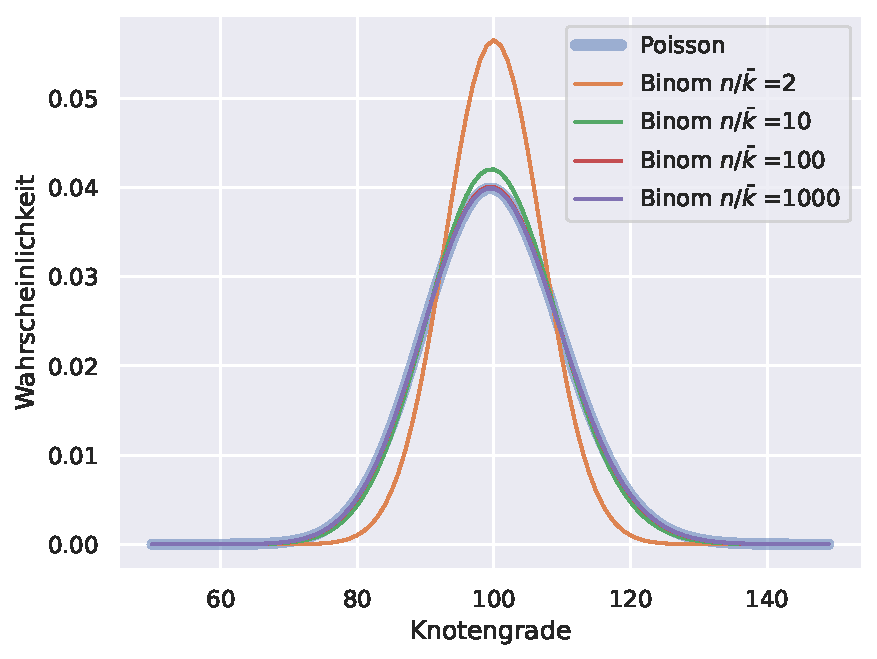
\includegraphics[width=0.5\textwidth]{data/binom_vs_poisson.pdf}
    \end{center}
    \caption{
        Vergleich von Binomialverteilung und Poissonverteilung für fixierten Durchschnittsgrad $\bar k = 100$.
        Je größer $n$, desto eher ist die Approximations-Voraussetzung $\bar k \ll n$ erfüllt und desto mehr sind Binomialverteilung und Poissonverteilung deckungsgleich.
    }
    \label{fig:binom_vs_poisson}
\end{figure}

\bigskip

Aus dieser Approximation mittels Poissonverteilung ergibt sich eine interessante Einsicht.
Während \aside{Für $\bar k \ll n$ ist die Gradverteilung nur von $\bar k$ abhängig} die Binomialverteilung von der Knotenanzahl~$n$ und Kantenwahrscheinlichkeit~$p$ abhängt, hat die Poissonverteilung nur den Parameter~$\lambda = p / (n-1) \approx \bar k$.
Die Interpretation hiervon ist, dass für $\bar k \ll n$ die Gradverteilung nur vom Durchschnittsgrad~$\bar k$, nicht aber von der Knotenanzahl im Graphen abhängen sollte.
\Cref{fig:binom_vs_poisson} untermauert diese Interpretation:
Die Binomialverteilungen der zwei größten Netze sind mit dem bloßen Auge nicht mehr von der Poissonverteilung unterscheidbar.

Diese Einsicht können wir uns wie folgt erklären:
Die Poissonverteilung beschreibt die Anzahl von Ereignissen, die innerhalb eines fixierten Intervalls auftreten, wenn die mittlere Rate konstant ist.
In diesem Bild ist jede Zeile der Adjazenzmatrix solch ein Intervall und die mittlere Rate entspricht der durchschnittlichen Anzahl an Einsen pro Zeile -- also dem Durchschnittsgrad~$\bar d$.

Beachte auch, dass die Varianz der Poissonverteilung mit $\var(X) = \bar d$ größer ist als die Varianz der Binomialverteilung $\var(X) = n p(1 - p) \approx \bar d (1 - \bar d / n )$, wobei der geklammerte Faktor kleiner als $1$ ist.

\section{Power-Law-Gradverteilung}
\begin{figure}
    \begin{center}
        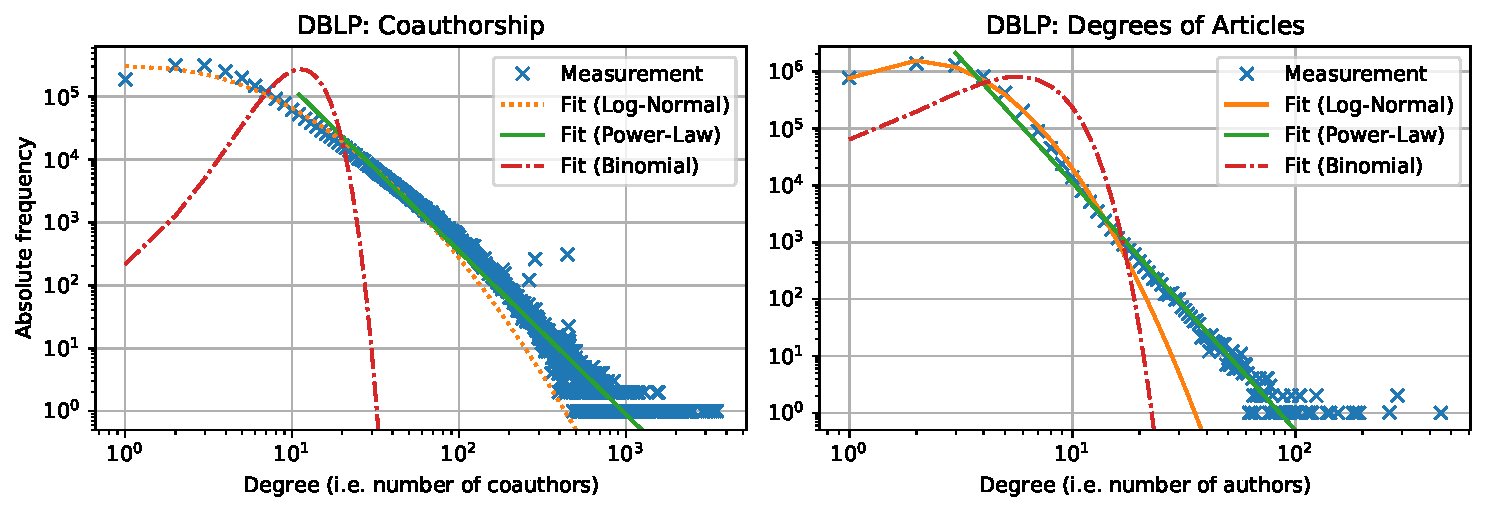
\includegraphics[width=\textwidth]{data/dblp_degree_distribution.pdf}
    \end{center}
    \caption{Gradverteilung von zwei beobachteten Netzwerken~\cite{Penschuck_2020} verglichen mit drei analytischen Verteilungen.}
    \label{fig:grade_in_dblp}
\end{figure}

In \cref{fig:grade_in_dblp} stellen wir die Gradverteilung (genauer: das Histogramm der Gradsequenz) zweier beobachteter Netzwerke dar.
Die genaue Herkunft der Graphen ist hier nicht wichtig; viele beobachte komplexe Netzwerke zeigen einen qualitativ ähnlichen Verlauf.
Was sofort auffällt, ist, dass die rot dargestellte Binomialverteilung keine satisfaktionsfähige Übereinstimmung mit der beobachteten Verteilung zeigt:

\begin{itemize}
    \item Die  Binomialverteilung sagt vorher, dass die meisten Knoten grob den Durchschnittsgrad haben müssten.
          Zu beiden Richtungen --~sprich für kleinere und größere Grade~-- sollte es deutlich weniger Knoten geben.

    \item Der \aside{Binomialverteilung und Poissonverteilung haben keine extremen Gerade.} maximale Grad ($\approx 30$ im linken Schaubild) sollte in etwa dieselbe Größenordnung haben wie der Durchschnittsgrad ($\approx 10$).
\end{itemize}

\noindent
Das beobachtete Netzwerk hat jedoch ein signifikant anderes Verhalten:
\begin{itemize}
    \item Die meisten Knoten haben sehr geringen Grad -- deutlich geringer als der Durchschnittsgrad.
    \item Der maximal Grad ($\approx 4000$) ist viel höher als der Durchschnittsgrad ($\approx 10$).
          Offensichtlich \qq{ziehen} diese wenigen Knoten den Durchschnittsgrad also maßgeblich nach oben.
          Es sollte daher auch nicht überraschend, dass diese sog. Hubs viele Eigenschaften des Netzwerks prägen.
\end{itemize}

In \cref{fig:grade_in_dblp} \aside{Power Law entspricht einer Geraden im Histogramm.} fällt ebenfalls auf, dass sich das Histogramm durch eine Gerade (im Folgenden als Linie bezeichnet, um Verwechselung mit Grad auszuschließen) relativ gut approximieren lässt.
Dies trifft besonders auf größere Grade zu -- aufgrund des doppellogarithmischen Plots stellen diese in absoluten Zahlen einen deutlich größeren Bereich dar, als die Abbildung suggeriert.
Wir können also als Arbeitshypothese annehmen, dass die meisten Knotengrade gut durch eine Linie im doppellogarithmischen Plot beschrieben werden.
Welche Gesetzmäßigkeit können wir daraus ableiten?

Wir können eine Linie mittels $y = mx + b$ beschreiben.
Im doppellogarithmischen Plot sind nun beide Achsen skaliert.
Es gilt daher $x = \log d$ und $y = \log h(d)$, wobei $d$ der Grad sei und $h(d)$ die Häufigkeit widerspiegele.
Dann gilt:
\begin{align}
    y               & = mx + b              \\
    \log h(d)       & = m\log d + b         \\
    \exp[\log h(d)] & = \exp[\log(d^m) + b] \\
    h(d)            & = \exp(b) \cdot d^m
\end{align}

Die Häufigkeit skaliert also proportional zu $d^m$.
Wir \aside{Potenzgesetz, Power Law: $p \propto d^{-\gamma}$ für (meist) $2 < \gamma < 3$} sprechen daher von einem Potenzgesetz (engl. Power Law).
Da die Anzahl der Beobachtungen für größere Grade abnimmt, ist der Exponent immer negativ.
Wir schreiben ihn daher als $d^{-\gamma}$, wobei der sog. \emph{Power Law Exponent}~$\gamma$ aus dem Intervall $2 < \gamma < 3$ stammt (falls nicht anders angegeben).

Um eine Wahrscheinlichkeitsverteilung $p(d)$ zu erhalten, müssen wir die Terme noch skalieren:
\begin{equation}
    p(d) = C' h(d) = \underbrace{C'\exp(b)}_{:= C} d^{-\gamma}
\end{equation}

\noindent
Wir absorbieren also den Faktor $\exp(b)$ in die Normierungskonstante~$C$:
\begin{align}
    1                & \stackrel{!}{=} \sum_{i=1}^\infty C i^{-\gamma}                          \\
    C                & = \frac{1}{\sum_{i=1}^\infty i^{-\gamma}}      = \frac{1}{\zeta(\gamma)} \\
    \nonumber                                                                                   \\
    \Rightarrow p(d) & = \frac{d^{-\gamma}}{\zeta(\gamma)}
\end{align}

Die Funktion $\zeta(\gamma)$ ist die sog. Riemann-Zeta-Funktion (wir werden diese im Folgenden nicht dediziert betrachten).

Beobachte, dass $0^a$ für $a < 0$ eine Division durch $0$ darstellt.
Daher ist $p(0)$ nicht definiert und wird explizit in der vorherigen Summierung herausgenommen.
Sollte ein Graph $n_0>0$ isolierte Knoten beinhalten, betrachtet man diese i.\,d.\,R. als Sonderfall.
Wir definieren also $p(0) = n_0 / n$ und skalieren die Power-Law-Verteilung auf $1  - n_0 /n$.

\def\dmin{\ensuremath{{d_{\text{min}}}}}
\def\dmax{\ensuremath{{d_{\text{max}}}}}
\def\dnc{\ensuremath{{d_{\text{nc}}}}}

Umgekehrt ist es oft auch sinnvoll, die minimalen und maximalen Grade $\dmin < \dmax$ explizit zu beschränken.
Wir müssen dann nur die Skalierungskonstante auf den kleineren Bereich anpassen:
\begin{equation}
    C_{\dmin,\dmax} = 1 / \smashoperator{\sum_{d = \dmin}^{\dmax}} d^{-\gamma}
\end{equation}

\begin{exercise}\label{aufg:dmin_dmax}
    Entwickele durch ein paar stichprobenartige Rechnungen eine Intuition, welchen Einfluss $\dmin$ und $\dmax$ auf $C_{\dmin,\dmax}$ haben.
    Erkläre deine Beobachtungen.
\end{exercise}

\subsection{Kontinuierlicher Formalismus}
In der Herleitung des diskreten Power Law haben wir bereits in der Normierung die transzendente Riemann-Zeta-Funktion $\zeta(\gamma)$ gesehen.
Weitere Analysen werden durch die diskrete Natur der Verteilung nicht einfacher.
Daher ist es oft bequemer, die Gradverteilung als kontinuierliches Konstrukt anzunehmen.
An der Grundform ändert sich dann erst einmal nichts, außer, dass der Grad nun eine strikt positive reelle Zahl sein darf:
\begin{equation}
    p(d) = C d^{-\gamma} \quad\quad d \in \mathbb R_{> 0}
\end{equation}

Für die Normierung steht uns nun aber das Integral statt der Summe zur Verfügung und führt zu deutlich handlicheren Ergebnissen.
Allerdings reicht es nicht mehr, nur $d = 0$ auszuschließen.
Wir definieren die Verteilung daher immer für einen expliziten minimalen Grad~\dmin; \dmax{} lässt sich analog einführen, wir verzichten aber darauf (siehe auch \cref{aufg:dmin_dmax}).

\begin{align}
    C_\dmin                           & = 1 / \int_{\dmin}^\infty d^{-\gamma} \intd d                                                \\
                                      & = 1 / \left[ \frac{1}{-\gamma + 1} d^{-\gamma + 1}  \right]_\dmin^\infty                       \\
                                      & = 1 / \left( - \frac{1}{-\gamma + 1} \dmin^{\textcolor{red}{1 - \gamma}}  \right)              \\
                                      & = \underbrace{( \gamma-1)}_{\mathclap{\textnormal{$> 0$ für $\gamma > 1$}}} \dmin^{\textcolor{red}{\gamma - 1}} \\
    \nonumber                                                                                                                          \\
    \Rightarrow\quad p_{\text{cont}}(d) & = (\gamma-1) \dmin^{\gamma - 1} \cdot d^{-\gamma}
\end{align}

Wichtig ist nun allerdings, dass $p_{\text{cont}}(d)$ keine natürliche punktweise Interpretation mehr hat.
Vielmehr müssen wir nun immer die Wahrscheinlichkeit, dass ein $X$ aus einem Intervall $[a, b]$ stammt, betrachten:
\begin{equation}
    \prob{a \le X \le b} = \int_{a}^b p_{\text{cont}}(d) \intd k
\end{equation}

\begin{exercise}
    Berechne den Erwartungswert der kontinuierlichen Power-Law-Verteilung mit fixierten Grenzen $0 < \dmin < \dmax \le \infty$.
\end{exercise}

\subsection{Größe von Hubs}\label{subsec:groesse_von_hubs}
Eine zentrale Motivation, von Poissonverteilungen abzurücken, war es, dass sie keine außergewöhnlich großen Grade zulassen.
Daher wollen wir den größten Grad eines Knotens in einer Power-Law-Verteilungen abschätzen.

Konkret suchen wir die Größe \dnc{} (engl. natural cut-off), bei der wir nur einen Knoten mit Grad $\ge \dnc$ erwarten.
Es muss also gelten, dass $\prob{\deg(u) \ge \dnc} = 1 / n$ ist:
\begin{align}
    1/n                                & = \int_\dnc^\infty p(d) \intd d                                                               \\
                                       & = C \int_\dnc^\infty d^{-\gamma} \intd d                                                      \\
                                       & = (\gamma-1) \dmin^{\gamma - 1} \left[ \frac{d^{-\gamma + 1}}{-\gamma +1} \right]_\dnc^\infty \\
                                       & = (\gamma-1) \dmin^{\gamma - 1} \left( 0 - \frac{\dnc^{-\gamma + 1}}{-\gamma +1} \right)      \\
                                       & = \dmin^{\gamma - 1} \dnc^{1 - \gamma}                                                        \\
    \nonumber                                                                                                                          \\
    \Rightarrow\quad \dnc^{\gamma - 1} & = \dmin^{\gamma - 1} n                                                                        \\
    \Leftrightarrow\quad \dnc          & = \dmin n^{1/(\gamma - 1)}
\end{align}

Für $\gamma  < 2$ sagt diese Gleichung einen Knoten voraus, der mehr Nachbarn hat, als es Knoten im Graphen gibt.
Dies ist nur eines von vielen Indizien, die zu unserer Annahme $\gamma > 2$ führen.
Für $\gamma \searrow 2$ (\dh rechtsseitiger Grenzwert für $\gamma \to 2$) skaliert der maximale Grad als $\Theta(n)$.
Für $\gamma = 3$ ist er noch $\Theta(\sqrt{n})$ et cetera.

\section{Wie entstehen Power-Law-Gradverteilungen?}
Das Entstehen von Power-Law-Verteilungen in unterschiedlichsten Netzwerken gibt Anlass zu der Frage, wie solche Verteilungen denn eigentlich entstehen.
Barab{\'{a}}si und Albert~\cite{barabasi1999emergence} geben eine sehr populäre Erklärung, die besonders durch ihre Simplizität besticht.
Ähnliche Techniken wurden jedoch bereits früher verfolgt (\zB~\cite{10.2307/1716232}).

Die beiden Autoren schlagen ein neues Modell vor, das wir im Folgenden BA-Modell nennen.
Es stellt zwei implizite Annahmen von \Gnp- und \Gnm-Graphen infrage:
\begin{itemize}
    \item
          In \Gnp-Graphen fixieren wir die Knotenanzahl initial und ändern diese dann nicht mehr.
          Netzwerke in der freien Wildbahn unterliegen jedoch in der Regel einer Dynamik:
          Knoten und Kanten kommen hinzu und verschwinden ggf. wieder.

    \item
          Wenn wir einen Knoten im \Gnp-Graphen als Spieler interpretieren, nimmt das Modell an, dass die Nachbarn rein zufällig ausgesucht werden.
          Tatsächlich unterliegen aber viele Handlungen im echten Leben einem sog. Bias (\dh einer verzerrten Wahrscheinlichkeitsverteilung).

          Dies ist besonders auffällig, wenn es zu einer Form von Selektion kommt.
          So kann kein Mensch alle Webseiten kennen (und dann darauf verlinken); von Facebook, Twitter und Google haben die Meisten aber gehört.
          Wenn also eine zufällige Person einen Artikel schreibt, ist es deutlich wahrscheinlicher, dass ein Link zu Twitter entsteht als ein Link zu einer bestimmten obskuren Webseite.
\end{itemize}

\subsection{Das BA-Modell}
Das \aside{BA-Modell beinhaltet Wachstum und Preferential Attachment.} BA-Modell trägt beiden Beobachtungen Rechnung.
Wir starten zunächst mit einem (meist) kleinen und zusammenhängenden Startgraphen mit $n_0$ Knoten und $m_0$ Kanten.
Dann fügen wir iterativ $N$ neue Knoten hinzu und erhalten so am Ende $n = n_0 + N$ Knoten.
Jeder neue Knoten verbindet sich mit $\nu \le n_0$ zufällig gewählten Nachbarn.
Wir sagen, dass der $t$-te neue Knoten im $t$-ten Zeitschritt (für $t = 1,2, \ldots, N$) hinzufügt wird;
unmittelbar nach dem $t$-ten Zeitschritt hat der Graph also
\begin{equation}
    n_t = n_0 + t \text{ Knoten} \quad \text{und} \quad
    m_t = m_0 + \nu t \text{ Kanten}.
\end{equation}
Analog bezeichnen wir den Grad eines Knotens $v$ nach Zeitschritt $t$ als $\deg_t(v)$.
Für $t \ggg n_0$ konvergiert das BA-Modell also gegen einen Durchschnittsgrad von
\begin{equation}
    \bar{d_t} = \frac{1}{n_t} \sum_{v} \deg_t(v) = 2 \frac{m_0 + \nu t}{n_0 + t} \to 2 \nu.
\end{equation}

Um den zuvor genannten Bias zu implementieren, nehmen wir aber an, dass Knoten mit vielen Nachbarn besonders bekannt sind, und unterstellen einen linearen Zusammenhang.
Wenn wir also aus zwei Knoten $a$ und $b$ mit $\deg(a) = 2\deg(b)$ wählen müssen, ziehen wir Knoten~$a$ mit doppelter Wahrscheinlichkeit.
Sei $p_t(v)$ die Wahrscheinlichkeit, dass wir Knoten $v$ in Zeitschritt $t + 1$ ziehen.
Dann gilt:
\begin{equation}
    p_t(v) = \frac{\deg_t(v)}{\sum_u  \deg_t(u)} = \frac{\deg_t(v)}{2(m_0 + \nu t)}
\end{equation}

\subsection{Dynamik in der Gradverteilung}
Der beschriebene Bias wird \emph{Preferential Attachment} bezeichnet.
Es bildet sich eine positive Rückkopplung:
Ein Knoten mit hohem Grad wird wahrscheinlicher als andere Knoten gezogen.
Ein gut vernetzter Knoten akkumuliert also schneller neue Nachbarn und wird dadurch noch berühmter.
Der Prozess liegt daher einigen Sprichwörtern zugrunde, \zB \qq{the rich get richer} (dt. \qq{Der Teufel \dots{} auf den größten Haufen}).
Es gibt diverse Methoden zur formalen Analyse des Prozess -- eine der einfachsten ist der kontinuierliche Formalismus, bei dem wir Knotengrade und die Zeit durch reelle Zahlen approximieren.
Der Einfachheit halber verwenden wir dennoch weiterhin den Begriff Zeitschritt, womit wir ein Zeitintervall von Einheitslänge meinen.

Wir gehen davon aus, dass die $\nu$ Kanten in einem Zeitschritt gleichzeitig gezogen werden;
es können also Mehrfachkanten entstehen.
Die erwartete Anzahl an Nachbarn, die Knoten~$v$ in einem Schritt~$t+1$ ansammelt, ist dann also $\nu p_t(v)$.
Da die Zeit ab jetzt kontinuierlich angenommen wird, \emph{fixieren wir einen Knoten $v_i$}, der zum Zeitpunkt $t_i$ hinzugefügt wird, und betrachten seinen Grad als zeitabhängige Funktion $d(t)$.
Es gilt $d(t) = 0$ für $t < t_i$ und $d(t_i) = \nu$.\footnote{
    Wir weichen an dieser Stelle von der diskreten Notation ab, bei der erst $d(t_i + 1) = \nu$ wäre.
    Dies hat aber keinen signifikanten Einfluss auf unsere Analyse und vereinfacht die Formeln.
}
Analog sei $m(t) = m_0 + \nu t$ die kontinuierliche Kantenanzahl.

Das Wachstum $\intd d(t) / \intd t$ der Funktion hängt nun vom Grad $d(t)$ selbst ab.
Es ergibt sich somit die folgende Differentialgleichung:
\begin{align}
    \frac{\intd d(t)}{\intd t}
     & = \nu p_t(v)
    = \nu \frac{d(t)}{2 m(t)}
    = \nu \frac{d(t)}{2(m_0 + \nu t)}                                         \\
     & \stackrel{\mathclap{t \gg 0}}{\approx} \nu \frac{d(t)}{2 \nu t} = \frac{d(t)}{2t}
\end{align}

Diese spezielle Differentialgleichung lässt sich relativ einfach lösen.
Wir teilen beide Seiten durch $d(t)$ (ab Zeitpunkt $t \ge t_i$ gilt $d(t) > 0$) und integrieren dann von $t_i$ (dem Zeitpunkt, zu dem der Knoten $v_i$ hinzugefügt wurde) bis $T$:
\begin{equation}
    \int_{t_i}^T  \frac{\frac{\intd d(t)}{\intd t}}{d(t)} \intd t = \int_{t_i}^T \frac{1}{2t} \intd t
\end{equation}

\noindent
Die rechte Seite ist ein Standardintegral:
\begin{equation}
    \int_{t_i}^T \frac{1}{2t} \intd t = \left[ \frac 1 2 \log t \right]_{t_i}^T = \frac 1 2 \log\left(\frac{T}{t_i}\right)
\end{equation}

Die linke Seite lässt sich mittels Substitution von $u = d(t)$ und $\intd u = \frac{\intd d(t)}{\intd t} \intd t$ analog zur rechten Seite integrieren.
Somit folgt insgesamt:
\begin{align}
    \log\left(\frac{d(T)}{d(t_i)}\right) & = \frac 1 2 \log \left(\frac{T}{t_i}\right)                             \\
    \frac{d(T)}{d(t_i)}                  & = \sqrt{\frac{T}{t_i}}                                                  \\
    d(T)                                 & = d(t_i) \sqrt{\frac{T}{t_i}} = \nu \left( \frac{T}{t_i} \right)^\beta,
\end{align}
wobei $\beta = 1/2$ als \aside{dynamischer Exponent $\beta = 1/2$} dynamischer Exponent bezeichnet wird.

Diese unscheinbare Gleichung gibt bereits viel über das Verhalten von BA-Netzwerken preis.
Zunächst fällt auf, dass der Grad monoton wächst (es gibt schließlich keinen Prozess, um ihn zu reduzieren).
Die erwartete Anzahl der Nachbarn von verschiedenen Knoten $v_i$ und $v_j$ unterscheidet sich zudem nur durch die Zeitpunkte $t_i$ und $t_j$, zu denen sie hinzugefügt wurden.
Je früher ein Knoten ins Netz eintrat, desto höher ist sein erwarteter Grad -- der sogenannte \aside{first-mover advantage} \emph{first-mover advantage}.

Die Situation für später hinzugekommene ist sogar noch schlechter, als man zunächst erwarten würde:
Die Startzeit~$t_i$ skaliert mit $\sqrt{1 / t_i}$ in den Knotengrad.
Während ein frühes Mitglied innerhalb einer gewissen Zeitspanne nach seinem Beitritt noch $X$ Nachbarn anhäufen konnte, bekommt ein späterer Knoten in derselben Zeit nur noch einen Bruchteil dieser Knoten.
Dies liegt einfach daran, dass es in späteren Zeitpunkten mehr \qq{Konkurrenz} gibt und somit Nachzügler kaum Aufmerksamkeit bekommen.
Dies kann man als Schwäche des Netzwerks interpretieren, da die einzige Chance, im Mittel erfolgreich zu sein, darin besteht, früh beigetreten zu sein.

\subsection{Gradverteilung des BA-Modells}
Im vorherigen Kapitel haben wir herausgefunden, dass der Grad eines Knotens~$v_i$ nach dem Beitritt ins Netz zu Zeitpunkt $t_i$ gemäß $d(t) = \nu (t  / t_i)^{1/2}$ wächst.
Wir müssen dieses Ergebnis noch in eine Gradverteilung zum Zeitpunkt $T \ggg 1$ übersetzen.

Die Intuition hierfür ist folgende:
Wir wissen, dass wir zum Zeitpunkt~$T$ insgesamt~$T$ zufällige Knoten hinzugefügt haben, und können annehmen, dass wir das in einem regelmäßigen Takt getan haben.
Dann müssen wir nur noch extrapolieren, welchen Grad wir für jeden dieser Knoten zu Zeitpunkt $T$ erwarten.
Konkret fragen wir uns, wann ein Knoten eingefügt werden musste, \sd er höchsten Grad $k$ hat:
\begin{alignat}{2}
                     &  & d(T)                                   & < k         \\
    \Leftrightarrow~ &  & \nu \left(\frac{T}{t_i}\right)^\beta   & < k         \\
    \Leftrightarrow~ &  & \frac{\nu}{k} T^\beta                  & < t_i^\beta \\
    \Leftrightarrow~ &  & \left(\frac{\nu}{k}\right)^{1/\beta} T & < t_i
\end{alignat}

Wir erwarten also, dass Knoten, die ab dem Zeitpunkt $t_i > (\nu / k)^{1/\beta} T$ eingefügt wurden, einen Grad von höchsten $k$ haben.
Davon gibt es $T - (\nu / k)^{1/\beta} T$ viele!
Sei $X$ nun der Grad eines zum Zeitpunkt~$T$ uniform gewählten Knotens und $P(k) = \prob{X \le k}$ die kumulative Verteilungsfunktion.
Dann gilt:
\begin{align}
    P(k) & = \prob{X \le k} = \frac{T - (\nu / k)^{1/\beta} T}{n_T} = \frac{T - (\nu / k)^{1/\beta} T}{n_0 + T} \\
         & \stackrel{\mathclap{T \ggg n_0}}{\approx} \quad\! \frac{T - (\nu / k)^{1/\beta} T}{T} = 1 - (\nu / k)^{1/\beta}
\end{align}

Für die Gradverteilung benötigen wir nun die Wahrscheinlichkeitsverteilung $p(k)$, also die Ableitung von $P(k)$:
\begin{align}
    p(k) & = \frac{\intd P(k)}{\intd k} = \frac{\intd}{\intd k} (1 - (\nu / k)^{1/\beta}) \\
         & = - \nu ^ {1/\beta}  \frac{\intd}{\intd k} k ^{-1/\beta}                       \\
         & = \frac{1}{\beta} \nu ^{1 / \beta} k^{-1/\beta - 1}                            \\
         & = 2 \nu^2 k^{-3}
\end{align}

Hierbei sind $2 \nu^2$ konstante Vorfaktoren.
Durch Parametervergleich ergibt sich also eine Power-Law-Verteilung mit Exponent $\gamma = 3$.

\section{Generieren von BA-Graphen}
BA-Graphen lassen sich mit einem überraschend einfachen Generator in in der Ausgabegröße linearer Zeit erzeugen.
Das Grundgerüst des Algorithmus~\cite{batagelj2005efficient} folgt dem BA-Modell.
Wir unterhalten eine Datenstruktur, die den wachsenden Graphen repräsentiert, und fügen dann iterativ Kanten hinzu.

Um zum Zeitpunkt~$t$ die $m_t$ Kanten zu speichern, nutzen wir ein Array~$A$ mit $2m_t$ Einträgen.
Die $i$-te Kanten $\set{u_i, v_i}$ wird dabei durch $A[2i - 1] = u_i$ und $A[2i] = v_i$ gespeichert.
Die zentrale Beobachtung ist nun, dass in $A[1 .. 2m_t]$ jeder Knoten $u$ genau $\deg_t(u)$ mal abgespeichert ist.
Wir müssen als nur einen Eintrag aus $A$ uniform zufällig ziehen, um die benötigte Verteilung zu erhalten.
Der vollständige Generator ist in \cref{alg:bb_ba} zusammengefasst.

Der Generator \cref{alg:bb_ba} hat jedoch eine praktische Schwäche:
Die $\nu$ Nachbarn eines Knotens werden unabhängig gezogen -- es kann also zu Mehrfachkanten kommen.
Dies ist in vielen Anwendungen unerwünscht.
Daher gehen wir im Folgenden davon aus, dass der Startgraph einfach ist (\dh, keine Mehrfachkanten enthält).

\begin{algorithm}[t]
	\KwIn{Startgraph als Kantenliste $E_0$ über Knoten $1, \ldots, n_0$. Anzahl der Zufallsknoten~$N$ sowie deren Nachbaranzahl~$\nu$.}
	\KwOut{Kantenliste $E$}
	\SetKwFunction{pushback}{pushBack}

	Allokiere leeres Array $E$ mit Kapazität $2(|E_0| + \nu N)$\;
	\ForEach{$\set{u,v} \in E_0$}{
		E.\pushback{$u$}\;
		E.\pushback{$v$}\;
		Gebe Kante $\set{u,v}$ aus und fahre fort\;
	}

	\For{$1 \le i \le N$}{
		\For{$1 \le j \le \nu$}{
			$x \gets $ uniform zufällig aus $E[1..2(|E_0| + \nu(i-1))]$\;
			E.\pushback{$x$}\;
			E.\pushback{$n_0 + i$}\;
			Gebe Kante $\set{x,n_0+i}$ aus und fahre fort\;
		}
	}
	\caption{Linearzeit-Generator~\cite{batagelj2005efficient} für BA-Graphen}
	\label{alg:bb_ba}
\end{algorithm}

Dann können wir Mehrfachkanten recht einfach erkennen:
Wir müssen nur die $\nu$ anfänglichen Nachbarn eines jeden neuen Knoten auf Duplikate prüfen.
(Warum reicht das?)
Es gibt zwei übliche Strategien, wenn wir Duplikate detektiert haben.

\begin{enumerate}
    \item Wenn wir einen Knoten $x$ mehrfach als Nachbar eines neuen Knotens~$v$ gezogen haben, \qq{löschen} wir alle bis auf eine resultierende Kante.
          Dies verändert zwar die Ausgabeverteilung, ist aber für große Ausgaben gar nicht so signifikant, da diese relativ selten auftreten (s.\,u.).

    \item Wir stellen sicher, dass wir $\nu$ verschiedene Nachbarn ziehen.
          Eine Technik hierfür haben wir bereits in \cref{sec:sampling_gnm} gesehen, um $k$ verschiedene Samples aus $N$ ohne Zurücklegen zu erstellen:
          Wir ziehen einfach für den neuen Knoten~$v$ unabhängig neue Nachbarn;
          wenn wir einen Nachbarn ziehen, der bereits mit $v$ verbunden ist, verwerfen wir diesen und versuchen es erneut.
          Mit dem gleichen Argument wie beim Löschen von Nachbarn hat dieses Verfahren keine Auswirkungen auf die erwartete asymptotische Laufzeit.

\end{enumerate}

\begin{exercise}
    Sei $G$ ein einfacher BA-Graph mit fixierten $\nu$ und $N \gg n_0$.
    Vereinfachend kann angenommen werden, dass $G$ vollständig der erwarteten Gradverteilung unterliegt.
    Schätze die erwartete Anzahl uniformen Stichproben ab, die benötigt werden, um $\nu$ verschiedene Nachbarn zu finden.
\end{exercise}

Wenn die Ausgabe in den Hauptspeicher des Computers passt, funktioniert der vorgestellte Algorithmus praktisch sehr gut.
In \cref{DBLP:conf/alenex/MeyerP16} werden zwei Algorithmen beschrieben, die über die Grenze hinweg funktionieren.

\subsection{Paralleles Ziehen von BA-Graphen}
Im Folgenden möchten wir uns zwei parallele Generatoren für BA-Graphen ansehen.
Vereinfachend betrachten wir nur $\nu = 1$; die Ideen lassen sich aber auch auf $\nu > 1$ verallgemeinern.

\subsubsection{Abhängigkeiten vermeiden}
Das Generieren von BA-Graphen wurde bis vor wenigen Jahren noch als \emph{inhärent sequentielles} Problem bezeichnet.
Jeder gezogene Knoten verändert die Gradverteilung, \sd sich zwischen den neu eingefügten Kanten Abhängigkeiten ergeben.
Allerdings gibt uns \cref{alg:bb_ba} bereits ein mentales Bild an die Hand, mit dem wir diese Abhängigkeiten in den Griff bekommen können.
Um die Beschreibung zu vereinfachen, gehen wir davon aus, dass jeder Eintrag im Array einer Kante entspricht (statt eigentlich zwei Einträgen pro Kante).
Dies ist eine asymptotisch nicht relevante Abschätzung zu unseren Ungunsten (siehe auch \cref{subsec:ba_sanders}).

Angenommen, wir haben bereits $\ell$ Kanten berechnet und diese in $E[1..\ell]$ geschrieben.
Dann können wir $p$ Kanten parallel bearbeiten, falls alle $p$ Kanten nur auf bereits bekannte Werte zugreifen.
In der Skizze korrespondiert dies zu der Situation, dass alle Kanten auf der rechten Seite der roten Linie nur Werte links von der roten Linie lesen.

\begin{center}
    \begin{tikzpicture}
        \foreach \x in {3, 6, ..., 120} {
                \path[draw=black, opacity=0.5] (\x mm, 0) to ++(0, 8mm);
            }
        \node[inner sep=0, minimum height=8mm, minimum width=120mm, draw, anchor=south west] at (0,0) {};

        \draw[thick, red] (99mm, -3mm) to ++(0, 14mm);
        \draw[brace down] (0, -5mm) to node[below=1ex] {Fertiggestellt} ++(98mm, 0);
        \draw[brace down] (100mm, -5mm) to node[below=1ex] {Parallel} ++(20mm, 0);

        \foreach \x/\l in {0/$1$, 96/$\ell$, 117/$\ell+p$} {
                \path[draw, ->] (\x mm + 1.5mm, 12mm) to ++(0, -3mm);
                \node[anchor=south] at (\x mm + 1.5mm, 12mm) {\l};
            }
    \end{tikzpicture}
\end{center}

Leider ist der einzige Wert, für den wir garantieren können, dass es zu keinerlei Abhängigkeiten kommt, $p=1$; nicht hilfreich.
Daher erweitern wir unseren Algorithmus um einen Fallback.

Bevor die $p$ Einträge berechnet werden, schreiben wir an die Stellen $E[\ell+1..\ell+p] \gets \bot$ einen besonderen Wert, der anzeigt, dass diese Zellen keine valide Kante enthält.
Dann ziehen wir unabhängig zufällig für jeden der $p$ neuen Einträge den Index~$s_i$, von dem gelesen werden soll.
Es gibt zwei Möglichkeiten:
\begin{itemize}
    \item Falls $s_i \le \ell$, gibt es keine Abhängigkeiten.
          Wir können $E[s_i]$ also sicher lesen, die neue Kante berechnen und das Ergebnis in $E[\ell + i]$ schreiben.
    \item Falls $s_i > \ell$, benötigen wir einen Wert, der gerade erst parallel berechnet wird.
          Wir lesen nun wiederholt von $E[s_i]$ bis wir einen Wert finden, der nicht $\bot$ ist.
          Dann berechnen wir unseren eigenen Eintrag und schreiben ihn nach $E[\ell +i]$.
          Jeden Versuch bezeichnen wir als Runde.
\end{itemize}

Um die Analyse einfach zu halten, nehmen wir an, dass die Prozessoren alle Standardoperation in konstanter Zeit ausführen können.
Weiter können wir am Ende jeder Runde in konstanter Zeit feststellen, ob alle Prozessoren fertig sind.
Für diese Annahmen ist das sog. CRCW-PRAM-Modell ein geeignetes Maschinenmodell.

Die schlechte Nachricht ist leider:
Der Algorithmus hat ein furchtbares Verhalten im worst case.
Für den Fall, dass $s_i = \ell + i - 1$ ist, hängt jede Kante von ihrem Vorgänger ab.
Pro \qq{Runde} des Fallback können wir also nur eine Kante produzieren.
Das ist nicht besser als ein sequentieller Algorithmus; wir verschwenden also $\Theta(p^2)$ Arbeit.
Die gute Nachricht ist aber, dass dies sehr unwahrscheinlich ist, wenn wir $p$ nicht allzu groß wählen.

\begin{lemma}\label{lem:par_ba_einzelschritt}
    Bei \aside{Es handelt sich hier um einen Spezialfall des Geburtstags\qq{paradoxon}.} einer vorhandenen Kantenliste $E$ mit $\ell = |E|$ können wir $p = \Oh{\sqrt{\ell}}$ Kanten parallel in erwarteter konstanter Zeit einfügen.
\end{lemma}

\begin{proof}
    Wir zeigen, dass die erwartete Anzahl an Abhängigkeiten extrem klein ist.
    Sei $Y_i$ eine Indikatorvariable mit $Y_i = 1 \Leftrightarrow s_i > \ell$:
    \begin{equation}
        \prob{Y_i = 1} = \prob{s_i > \ell} = \frac{i - 1}{\ell + i - 1}
    \end{equation}

    \noindent
    Somit folgt die erwartete Anzahl von Abhängigkeiten als
    \begin{align}
        \expv{\sum_{i=1}^p Y_i} & = \sum_{i=1}^{p} \frac{i - 1}{\ell + i - 1} \\
                                & = \sum_{i=0}^{p-1} \frac{i}{\ell + i}       \\
                                & \le p \frac{p}{\ell + p}                    \\
                                & \le \frac{p^2}{\ell}
    \end{align}

    \noindent
    Für $p = \Oh{\sqrt{\ell}}$ können wir also den Erwartungswert durch $\Oh{1}$  beschränken.
\end{proof}

Basierend auf \cref{lem:par_ba_einzelschritt} können wir nun mehrere Epochen aufbauen.
In der ersten Epoche starten wir mit $e_1 = \ell$ Kanten und fügen $\sqrt{\ell}$ neue hinzu.
In der nächsten Epoche haben wir dann schon $e_2 = \ell + \sqrt{\ell}$ und können schon $\sqrt{\ell + \sqrt{\ell}}$ neue Ergebnisse erzielen.
Es gilt also:
\begin{equation}
    e_i = \begin{cases*}
        \ell                     & falls $i = 1$, \\
        e_{i-1} + \sqrt{e_{i-1}} & sonst.
    \end{cases*}
\end{equation}

Da jede Epoche in Erwartung eine Laufzeit von $\Oh{1}$ hat, hängt also die Laufzeit des Gesamtalgorithmus von der Anzahl notwendiger Epochen ab.

\begin{lemma}
    Für $e_1 = \sqrt{m}$ können wir $m$ Kanten in $\Oh{\sqrt{m}}$ Epochen erzeugen.
\end{lemma}

\begin{proof}
    Beginnen wir einfacher: Wie viele Epochen benötigen wir höchstens, um von $e_1$ Kanten auf $2e_1$ Kanten zu kommen?
    Wir unterschätzen die Anzahl neuer Kanten pro Epoche durch $\sqrt{e_1}$ (also der Zuwachs aus der ersten Epoche).
    Dann sind wir nach $\sqrt{e_1}$ Epochen am Ziel $e_1 + \sqrt{e_1} \sqrt{e_1} = 2 e_1$.

    Dieses Vorgehen wiederholen wir logarithmisch oft.
    Vorsicht ist aber geboten, da wir, um von $2e_1$ nach $2(2e_1)$ zu kommen, $\sqrt{2 e_1}$ (statt wie vorher nur $\sqrt{e_1}$) Epochen benötigen.
    Sei $k$ die Anzahl an notwendigen Epochen, \dh $e_k \ge m$.
    Es folgt:

    \begin{align}
        k & \le \smashoperator[r]{\sum_{i=0}^{\ld(m/e_1)}} \sqrt{2^i e_1}      \\
          & = \sqrt{e_1} \smashoperator[r]{\sum_{i=0}^{\ld e_1}} 2^{i/2}       \\
          & \le \sqrt{e_1} 2 \smashoperator[r]{\sum_{i=1}^{(1+\ld e_1)/2}} 2^i \\
          & = \sqrt{e_1} \Oh{2^{2 + (\ld e_1) / 2}}         \\
          & = \sqrt{e_1} \Oh{\sqrt{e_1}} = \Oh{e_1}
    \end{align}
\end{proof}

Wir können also mit einem sequentiellen Algorithmus starten und in Zeit $\Oh{\sqrt m}$ einen Graphen generieren, der hinreichend groß ist, um in den parallelen Betrieb zu wechseln.
Ab dann ziehen wir die verbleibenden $m - \sqrt{m}$ Kanten in erwarteter Zeit $\Oh{\sqrt m}$.

\subsubsection{Abhängigkeiten beherrschen}\label{subsec:ba_sanders}
Im vorherigen Kapitel haben wir eine allgemeine Technik gesehen, um sequentielle Algorithmen mit geeigneten zufälligen Zugriffsmustern zu parallelisieren.
Wir konstruieren kleine Epochen, um Abhängigkeiten möglichst zu vermeiden und behandeln dennoch auftretende Abhängigkeiten als Sonderfall.

Für BA-Graphen im Speziellen zeigen~\cite{SANDERS2016489} jedoch, dass wir sogar $\Theta(m)$ Prozessoren sinnvoll Arbeit zukommen lassen und einen BA-Graphen mit hoher Wahrscheinlichkeit in $\Oh{\log m}$ Zeit erzeugen können.
Betrachten wir noch einmal die \qq{echte} Kantenliste, in der jede Kante aus zwei Einträgen besteht:

\begin{center}
    \begin{tikzpicture}
        \foreach \x in {0, 6, ..., 114} {
                \node[inner sep=0, minimum height=8mm, minimum width=3mm, fill=black!30, anchor=south west] at (\x mm, 0) {};
            }
        \foreach \x in {6, 12, ..., 114} {
                \path[draw] (\x mm, -2mm) to ++(0, 12mm);
            }
        \node[inner sep=0, minimum height=8mm, minimum width=120mm, draw, anchor=south west] at (0,0) {};
    \end{tikzpicture}
\end{center}

Jede Kante besteht aus einem trivialen \qq{deterministischen} Eintrag, nämlich dem Index des neuen Knotens, der sich aus dem Kantenindex ableiten lässt, und einem zufälligen Wert (hier weiß).
Wir nehmen nun an, dass jeder Kante~$i$ ein eigener Prozessor~$p_i$ zugeordnet ist.
Kanten aus dem Startgraph kopieren einfach den entsprechenden Wert.
Danach führen alle anderen Prozessoren folgendes Programm parallel aus:

\smallbreak
\RestyleAlgo{tworuled}
\begin{algorithm}[H]
    $E[2i - 1] \gets$ Knoten-ID des neuen Knotens\;
    $E[2i] \gets \bot$\;
    \BlankLine
    $s_i \gets $ uniform zufällig aus $\set{1 \ldots 2(i-1)}$\;
    \While{$E[s_i] = \bot$}{
        Warte auf nächste Runde\;
    }

    $E[2i] \gets E[s_i]$\;
\end{algorithm}
\RestyleAlgo{ruled}
\smallbreak

Dieser Algorithmus funktioniert so gut, weil sich in jeder Runde die erwartete Anzahl an nicht fertiggestellten Kanten halbiert.
Nach der ersten Runde sind alle Kanten fertig, deren $s_i$ ungerade war;
in diesem Fall konnten wir nämlich einfach die \qq{deterministische} Hälfte einer Kante lesen.
Da $s_i$ uniform gezogen wurde, ist $s_i$ mit Wahrscheinlichkeit $1/2$ ungerade.

In der zweiten Runde können wir von den verbleibenden Kanten all jene fertigstellen, die auf eine Kante zeigen, die in der ersten Runde fertig gestellt wurde.
In anderen Worten: Solche Kanten haben ein gerades $s_i$, das auf ein ungerades $s_{s_i}$ zeigt -- dies betrifft in Erwartung $1/4$ aller Kanten.

In der $i$-ten Runde setzt sich die Kette analog fort.
Insgesamt benötigen wir $i-1$ Verweise von gerade auf gerade, gefolgt von einem einzelnen auf ungerade.

Die erwartete Anzahl der Runden der letzten Kante ist also geometrisch mit Erfolgswahrscheinlichkeit $1/2$ verteilt.
In Erwartung sind wir für diese Kante nach $2$ Runden fertig.
Mittels Chernoff-Ungleichung können wir die Wahrscheinlichkeit, mehr als $\beta \log \nu N$ Runden zu benötigen, für geeignetes~$\beta$ auf $(\nu N)^{-2}$ beschränken.
Durch Union-Bound folgt dann, dass der Algorithmus mit hoher Wahrscheinlichkeit eine Laufzeit von $\Oh{\log \nu N}$ hat.

\subsubsection{Abhängigkeiten ausschließen}
Der eben vorgestellte Algorithmus kann auch so abgeändert werden, dass es zu keinerlei expliziten Abhängigkeiten kommt.
Dazu vermeiden wir es einfach, vollständig zufällige Vorgänger zu lesen.
Dies ist vor allem im Kontext von verteilten Multicomputern von Vorteil, bei denen Zugriffe auf den Speicher von anderen Computern typischerweise zu erheblicheren Verlangsamung führen.

Die Idee ist simpel: Statt von einer Position der Kantenliste zu lesen, ziehen wir einfach die Berechnung, die dort stattgefunden haben muss, selbst nach.

Angenommen wir befinden uns an Position~$i$ und ziehen~$s_i$.
Falls $s_i$ ungerade ist, befindet sich dort der Index eines neuen Knotens, den wir einfach nachrechnen können.
Falls $s_i$ gerade ist, müssen wir \qq{nur} denselben zufälligen Vorgänger~$s_{s_i}$ ziehen, der am Index $s_i$ gezogen wurde.

Dieses Oxymoron können wir lösen, indem wir die deterministische Natur unserer Pseudo-Zufallsgeneratoren ausnutzen.
Wir erzeugen an jeder Position der Kantenliste einen Pseudo-Zufallsgenerator, dessen Zustand deterministisch von der Position in der Kantenliste abgeleitet werden kann.
Man könnte beispielsweise einfach den Index als Seedwert für den Generator nutzen.

Hierbei müssen wir allerdings vorsichtig sein, da Pseudo-Zufallsgeneratoren in der Regel eine sogenannte Burn-in-Phase benötigen, da die ersten Werte ungewünschte Eigenschaften besitzen können.
Außerdem ist das Erzeugen eines Zufallszahlengenerators oft sehr viel teurer als das Ziehen eines Zufallswortes.
Daher nutzen die Autoren~\cite{SANDERS2016489} statt eines dedizierten Pseudo-Zufallsgenerator eine zufällige Hashfunktion.

Dies ist eine pragmatische Entscheidung und liefert --~je nach Hashfunktion~-- ein vergleichsweise kleines Ensemble an möglichen Ausgaben.
Empirisch scheinen aber die erzeugten Graphen ähnlich zu BA-Graphen zu sein.
Daher kann der Generator --~gerade bei verteilten Berechnungen~-- das Mittel der Wahl sein.

\subsection{Skalenfreie Netze}
Skalenfreie Netz (scale-free network) sind Graphen mit Power-Law-Gradverteilungen (Gegendarstellung: \cite{doi:10.1073/pnas.200327197});
hierbei handelt es sich um einen sehr gebräuchlichen Begriff in der Network-Science-Literatur.
Der Begriff selbst hat zwei (verwandte) Erklärungen, die uns noch einen Einblick in die Eigenschaften von Power-Law-Verteilungen erlauben.

\subsubsection{Skaleninvariant}\label{subsec:scaleinvariant}
Wir können \qq{skalenfrei} als \qq{skaleninvariant} auffassen.
Damit wird auf die Selbstähnlichkeit der Power-Law-Verteilung hingewiesen:
eine perfekte Power-Law-Verteilung ist in einem doppellogarithmischen Plot immer eine Gerade mit Steigung $-\gamma$.
Dabei ist unerheblich, wie groß das zugrunde liegende Objekt (hier: Knotenmenge) ist.

Wir können also die Verteilung umskalieren, also \zB die Knotenanzahl um einen Faktor $a$ vergrößern.
Dann gilt für entsprechende Zufallsvariable $X$ und $X'$:

\begin{alignat}{2}
    \prob{X = k}   &                                                                                                                                  && \propto k^{-\gamma}  \label{eq:prop-scalefree-1} \\
    \prob{X' = ak} & \propto (ak)^{-\gamma} = \underbrace{a^{-\gamma}}_{\mathclap{\substack{\text{von $k$} \\ \text{unabhängig}}}} \cdot\ k^{-\gamma} && \propto k^{-\gamma}\label{eq:prop-scalefree-2}
\end{alignat}

Beobachte, dass die Proportionalität in den \cref{eq:prop-scalefree-1,eq:prop-scalefree-2} jeweils andere Normierungen verbirgt.

\subsubsection{Unbegrenztes Wachstum}
Der Begriff \qq{scale-free network} wird regelmäßig Barab{\'{a}}si und Albert, den Autoren des BA-Modells, zugeschrieben.
Barab{\'{a}}si selbst erklärt den Begriff über das unbeschränkte Wachstum des $k$-ten Moments der Power-Law-Verteilung für $n \to \infty$.

Das $k$-te Moment einer kontinuierlichen (Grad-)Verteilung $p(d)$ ist definiert als:
\begin{equation}
    \langle d^k \rangle = \expv{X^k} = \int_\dmin^\dmax d^k p(d) \intd d,
\end{equation}
wobei $X \follows p$ eine nach $p$-verteilte Zufallsvariable ist.

Für $k=1$ erhalten wir also den Erwartungswert, $\langle d^2 \rangle$ ist essentiell in der Berechnung der Varianz $\langle d^2 \rangle - \langle d \rangle^2$, $\langle d^3 \rangle$ beeinflusst die Schiefe (skewness) et cetera.
Bezogen auf Power-Law-Verteilungen ergibt sich für $\gamma \neq k + 1$
\begin{align}
    \langle d^k \rangle
    & = \int_\dmin^\dmax d^k C d^{-\gamma} \intd d
    = C \left[ \frac{1}{k + 1 - \gamma} \cdot d^{k + 1 -\gamma}\right]_\dmin^\dmax    \\
    & = C \cdot \frac{\dmax^{k + 1 -\gamma} - \dmin^{k + 1 -\gamma}}{k + 1 - \gamma}
\end{align}
und für $\gamma = k + 1$
\begin{equation}
	\langle d^k \rangle
	= \int_\dmin^\dmax d^k C d^{-\gamma} \intd d
	= \int_\dmin^\dmax \frac{C}{d} \intd d
	= C \left( \ln \frac{\dmax}{\dmin} \right).
\end{equation}

Das Verhalten des $k$-ten Moments für $n \to \infty$ (und dadurch $\dmax \to \infty$) wird also maßgeblich durch $k + 1 - \gamma$ beschrieben:
\begin{itemize}
    \item Für $k + 1 < \gamma$ konvergiert $\lim_{\dmax \to \infty} \dmax^{k + 1 -\gamma} = 0$.
          Somit ist $\langle d^k \rangle$ endlich.

    \item Für $k + 1 = \gamma$ ist das $k$-te Moment konstant.

    \item Für $k + 1 > \gamma$ divergiert das $k$-te Moment und wächst grenzenlos.
\end{itemize}

\noindent
Bisher nahmen wir $2 < \gamma \le 3$ an.
In diesem Regime konvergiert $\langle d \rangle$, somit erwarten wir, dass der Durchschnittsgrad in einem wachsenden Netz irgendwann stagniert.
Dies widerspricht aber scheinbar unserer Analyse in \cref{subsec:groesse_von_hubs}, wo wir zeigten, dass der Grad von Hubs polynomiell in der Knotenanzahl wächst.
Dem wird aber schlicht dadurch Rechnung getragen, dass die Varianz über das divergierende zweite Moment $\langle d^2 \rangle$ wächst.
Polemisch gesagt, werden also Hubs als Ausreißer verbucht.
Ein zufällig gezogener Knoten kann kleinen oder großen Grad haben mit einer Streuung über viele Größenordnungen -- es gibt also kein Konzept von Größenverhältnissen (engl. scale).


\cleardoublepage
\fancyhead[LE]{Bibliographie}
\fancyhead[RO]{}
\thispagestyle{fancy}
\pagestyle{fancy}
\bibliographystyle{plainurl}
\small
\patchcmd{\thebibliography}{\chapter*}{\section*}{}{}
\bibliography{referenzen}
\end{document}
